\expandafter\ifx\csname ifdraft\endcsname\relax
 \begin{document}
\fi

\section{製作}

\subsection{装置全体の構成}

装置全体の構成を図\ref{fig:connection_map}に示す.

\begin{figure}[H]
  \begin{center}
    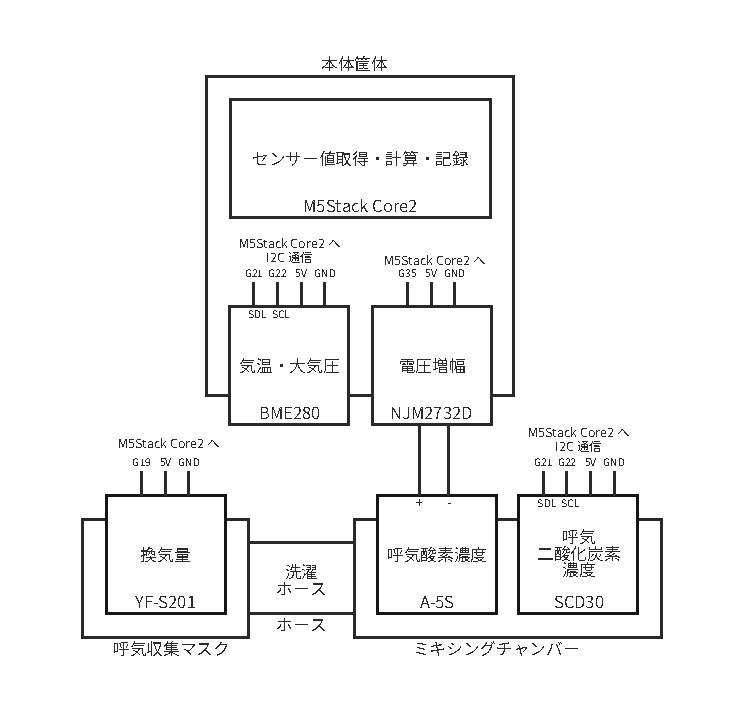
\includegraphics[width=12cm]{fig/connection_map}
    \caption{装置の全体構成}
    \label{fig:connection_map}
  \end{center}
\end{figure}

\subsubsection{マイコン}

センサー類を接続し,その値から各種計算値を求める本体となるマイコンには,M5Stack Core2を使用した.M5StackはESP32をベースに各種IOに加えてバッテリーや各種センサーなどを搭載した深センのM5Stack社によって開発されるマイコンである.ESP32の標準機能として無線LAN, Bluetoothのワイヤレス機能を搭載するため,インターネットを活用したIoT機器の開発を容易に行うことができる.

今回の装置は多数のセンサーを接続し,リアルタイムでの数値の計算・表示を行うことになる.そのため,入出力ピンの数が多く,同時多数のセンサーを接続することができるという理由からM5Stack Core2を使用した.M5Stack Core2はシリーズの中でも特に処理能力が高く,大型のタッチスクリーンとデータの書き込みが可能なTFカード(Micro SDカード)スロットを搭載する.図\ref{fig:m5stack_core2}にM5Stack Core2と\ref{tb:m5stack_core2_specsheet}にその仕様を示す.

\begin{figure}[H]
  \begin{center}
    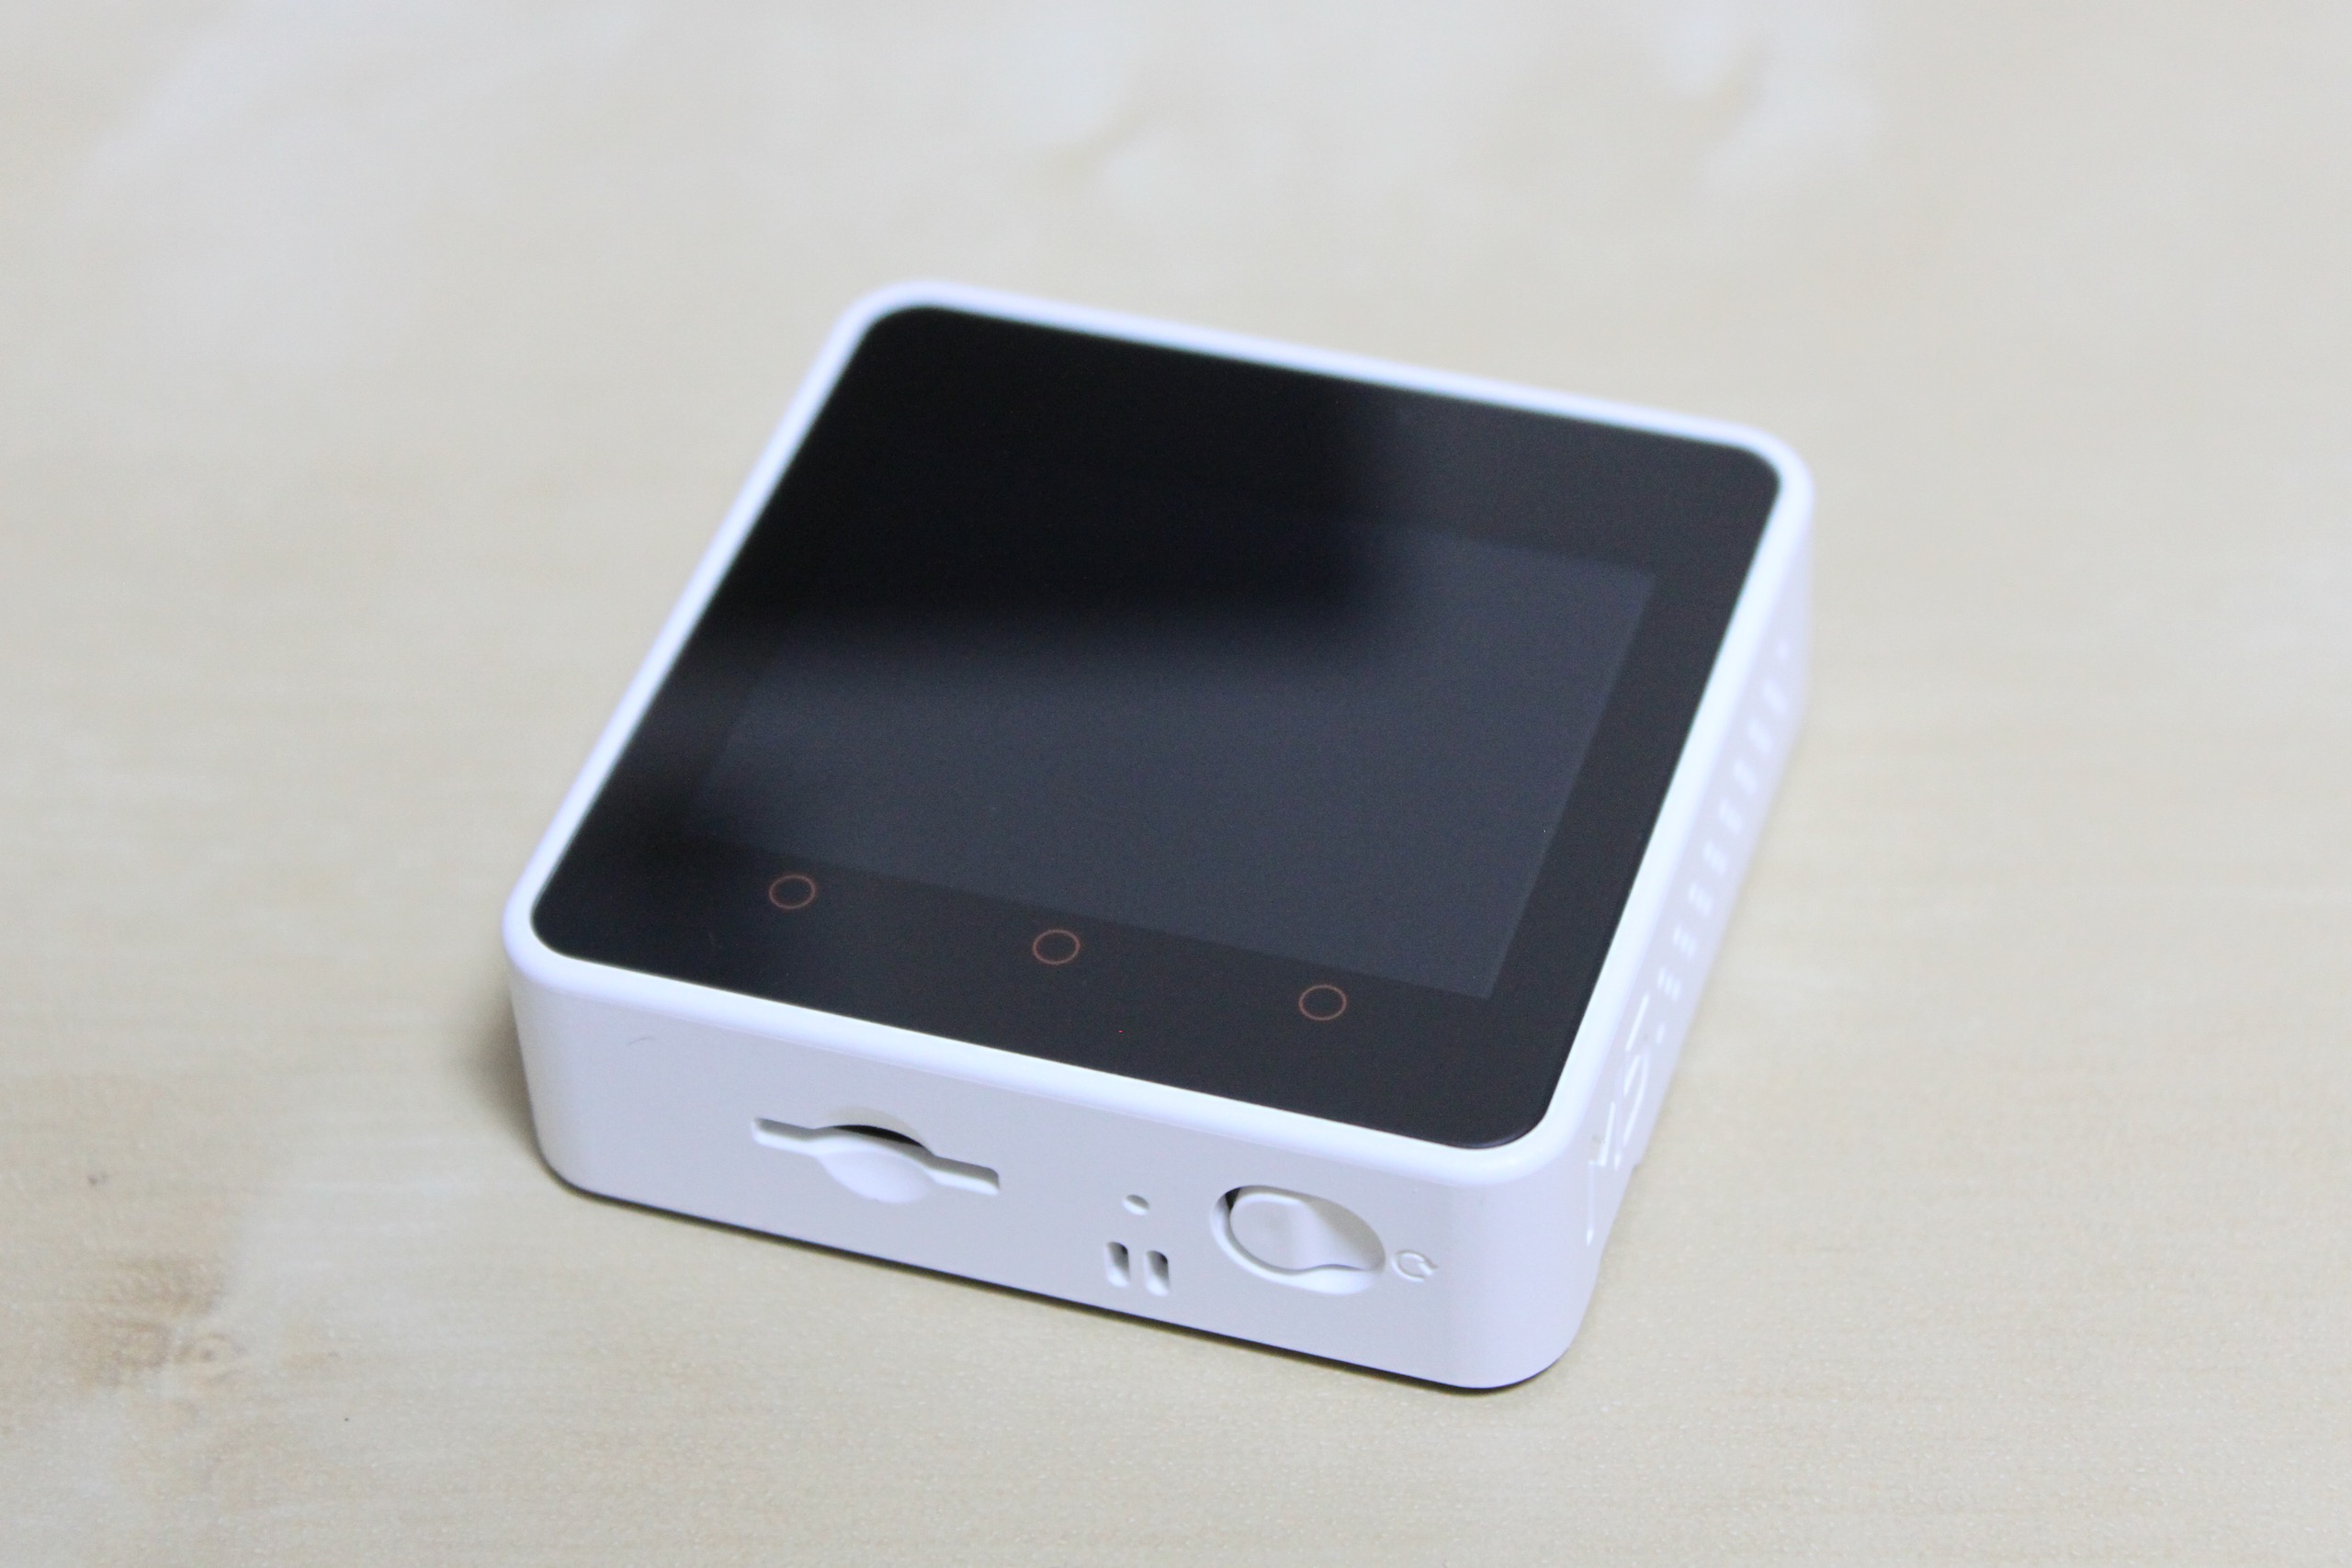
\includegraphics[width=8cm]{fig/m5stack_core2}
    \caption{M5Stack Core2}
    \label{fig:m5stack_core2}
  \end{center}
\end{figure}

\begin{table}[H]
\begin{center}
\caption{M5Stack Core2 主な仕様(スイッチサイエンス\cite{switchscience_m5stack_core2}より)}
\label{tb:m5stack_core2_specsheet}
\begin{tabular}{|l|l|}
\hline
リソース       & パラメータ                          \\ \hline
ESP32-D0WD-V3 & \begin{tabular}[c]{@{}l@{}}240 MHzデュアルコア,600 DMIPS,520 KB SRAM,\\ Wi-Fi,デュアルモードBluetooth\end{tabular} \\ \hline
フラッシュメモリ   & 16 MB                          \\ \hline
PSRAM      & 8 MB                           \\ \hline
入力電圧       & 5 V @ 500 mA                   \\ \hline
インターフェース      & USB Type-C \times 1, GROVE(I2C+I/O+UART) \times 1                                                     \\ \hline
IPS LCD スクリーン & 2.0インチ@320 \times 240 ILI9342C                                                                        \\ \hline
タッチスクリーン   & FT6336U                        \\ \hline
スピーカー      & 1W-0928                        \\ \hline
LED        & 電源表示灯(緑)                       \\ \hline
ボタン        & 電源ボタン,リセットボタン,静電容量ボタン \times 3 \\ \hline
バイブレーション機能 & 振動モーター                         \\ \hline
マイクロフォン    & SPM1423                        \\ \hline
I2Sパワーアンプ  & NS4168                         \\ \hline
6軸IMU      & MPU6886                        \\ \hline
RTC        & BM8563                         \\ \hline
PMU        & AXP192                         \\ \hline
USBチップ     & CP2104                         \\ \hline
DC/DC昇圧    & SY7088                         \\ \hline
TFカードスロット  & 最大16 GB                        \\ \hline
リチウムバッテリ   & 390 mAh @ 3.7 V                \\ \hline
アンテナ       & 2.4 GHz 3D アンテナ                \\ \hline
動作温度       & 0°C~40°C                       \\ \hline
正味重量       & 52 g                           \\ \hline
総重量        & 70 g                           \\ \hline
製品寸法       & 54 \times 54 \times 16 mm      \\ \hline
包装寸法       & 75 \times 60 \times 20 mm      \\ \hline
ケース素材      & プラスチック(PC)                     \\ \hline
\end{tabular}
\end{center}
\end{table}

\subsubsection{本体筐体}

M5Stack Core2とオペアンプによる電圧増幅回路(\ref{sec:opamp}),温度・大気圧センサー(\ref{sec:measuring_ambient}),各センサーとM5Stack Core2を接続するためのケーブルを収めるための筐体を3Dプリンターで製作した.筐体は上下2分割の構造とし,ネジ留めで一体化させる構造とした.下部のパーツに電圧増幅回路を実装したユニバーサル基板,温度・大気圧センサーをネジ留めし,その上にM5Stack Core2を乗せる.上部のパーツを共締めすることでM5Stack Core2を固定する構造である.図\ref{fig:enclosure}に今回製作した筐体を示す.

\begin{figure}[H]
  \begin{center}
    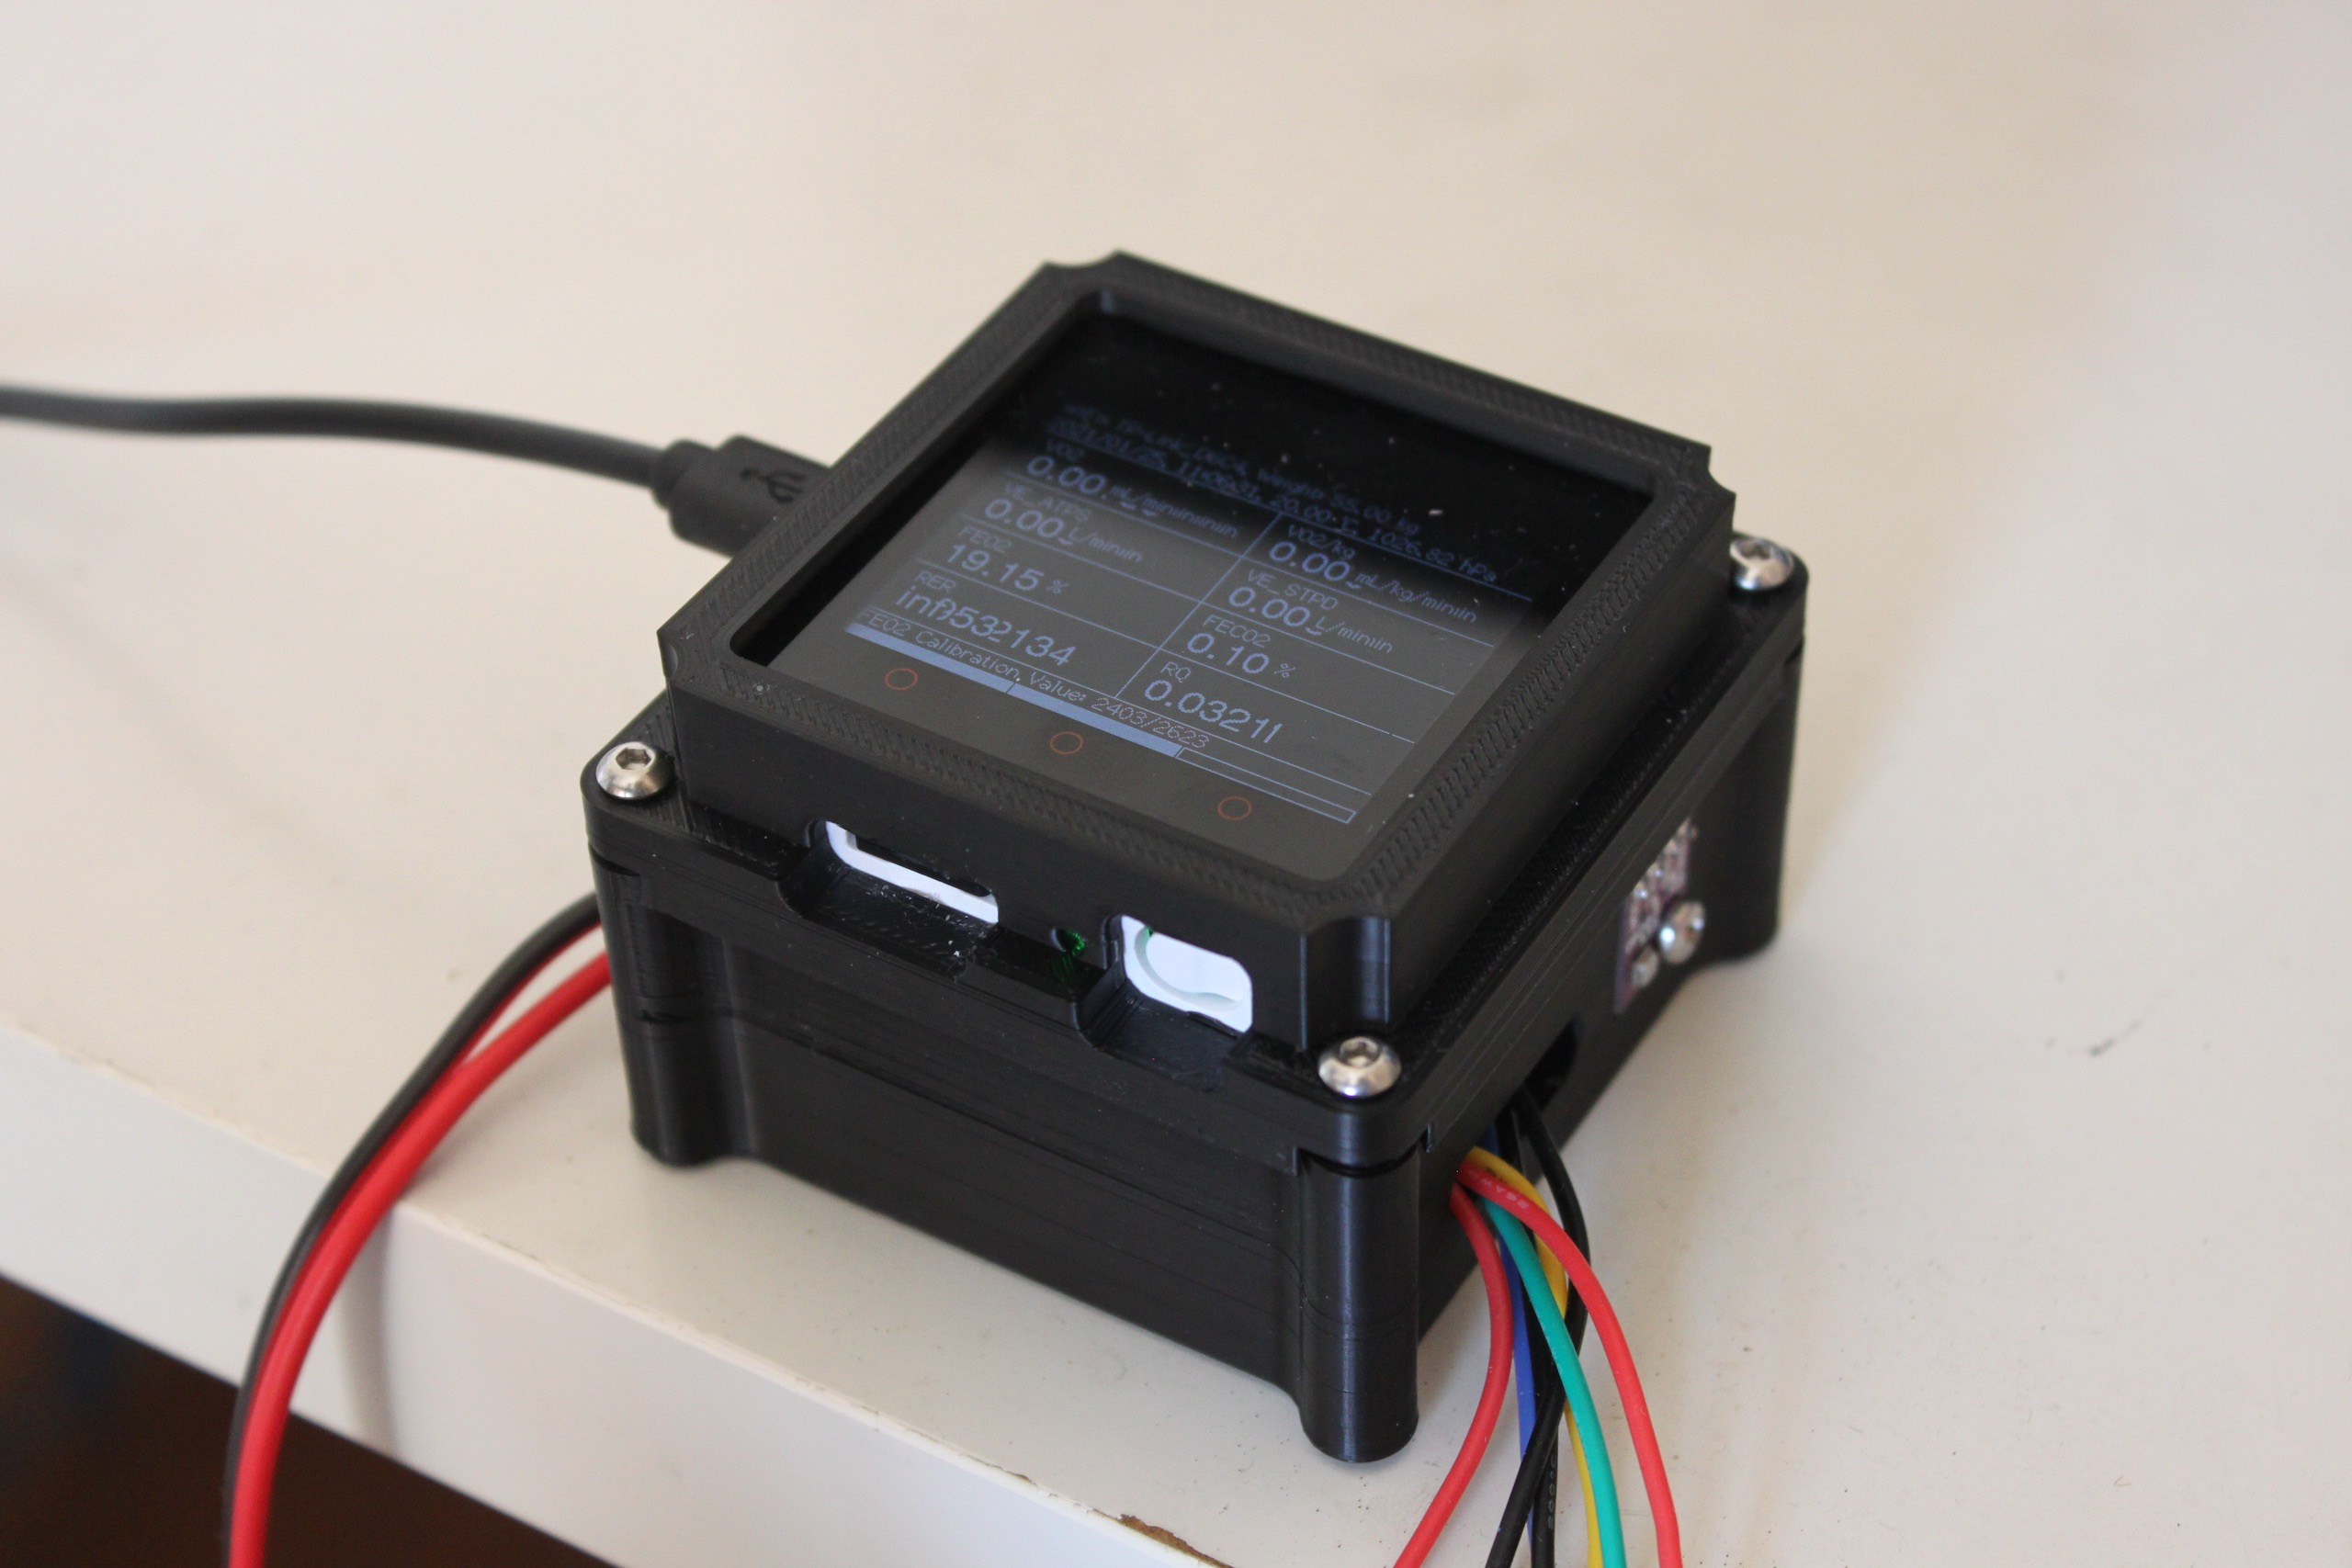
\includegraphics[width=8cm]{fig/enclosure}
    \caption{M5Stack,ユニバーサル基板,ケーブルを収めるための筐体}
    \label{fig:enclosure}
  \end{center}
\end{figure}

\subsection{呼気の収集}
\label{sec:correct}

\subsubsection{呼気収集の方法}
\label{sec:correct_method}

呼気の収集方法には,ダグラスバッグ法,ミキシングチャンバー法,ブレスバイブレス法などがある.それぞれ換気量の測定方法と呼気内の酸素と二酸化炭素の濃度の測定(呼気組成の測定)方法が異なる.各方法の特徴を表\ref{tb:correct_exhalation}にまとめた.

\begin{table}[H]
\begin{center}
\caption{呼気収集各方法の特徴}
\label{tb:correct_exhalation}
\scalebox{0.6}{
\begin{tabular}{|l|l|l|l|l|}
\hline
 &
  換気量の測定 &
  呼気組成の分析 &
  呼気気流抵抗 &
  特徴 \\ \hline
ダグラスバッグ法 &
  \begin{tabular}[c]{@{}l@{}}収集後に\\ ガスメーターで測定\end{tabular} &
  \begin{tabular}[c]{@{}l@{}}収集後に\\ バッグごとに分析\end{tabular} &
  小さい &
  \begin{tabular}[c]{@{}l@{}}単純な方法で精度が高い\\ 測定の労力が大きい\end{tabular} \\ \hline
ミキシングチャンバー法 &
  \begin{tabular}[c]{@{}l@{}}収集中に\\ 流量計で測定\end{tabular} &
  \begin{tabular}[c]{@{}l@{}}収集中に\\ チャンバー内で分析\end{tabular} &
  大きい &
  \begin{tabular}[c]{@{}l@{}}測定の方法により誤差を生じやすい\\ 測定の労力が小さい\end{tabular} \\ \hline
\begin{tabular}[c]{@{}l@{}}ブレスバイブレス法\\ (全自動分析法)\end{tabular} &
  \begin{tabular}[c]{@{}l@{}}収集中に\\ 呼吸ごとに流量計で測定\end{tabular} &
  \begin{tabular}[c]{@{}l@{}}収集中に\\ 呼吸ごとに分析\end{tabular} &
  大きい &
  \begin{tabular}[c]{@{}l@{}}複雑な方法ゆえ誤差を生じやすい\\ 測定の労力が小さい\end{tabular} \\ \hline
\end{tabular}
}
\end{center}
\end{table}

ダグラスバッグ法は,呼気ガスをダグラスバッグ(Douglas Bag)と呼ばれる大型のバッグに収集する方法である.この方法では,呼気量の測定は収集の完了後にガスメーターを接続し,バッグ内の呼気を全て出し切ることで行う.呼気の組成はこのうちの一部のサンプルを分析することで求める.時間変化を見る測定を行う場合は,時間ごとにバッグを取り換える必要がある.この方法は実験室における酸素摂取量の測定には古くから使われてきた方法である.バッグの取り替え時の操作により生じる誤差以外では大きな誤差が生じにくく,精度が高い方法とされている.大掛かりな機材と多数の検者を必要とするため,個人での測定には不向きであると言える.

ミキシングチャンバー法は,呼気ガスをミキシングチャンバーと呼ばれる混合気室に貯める方法である.ミキシングチャンバーは,ガス流路に適切な障害物を置くことで時間的に変化する呼気流を一定に均し,ガス濃度を平均化する機構である\cite{whats_mixing_chamber}.この方法では,呼気量の測定は集気マスクとミキシングチャンバー間の流路に設置した流量計で行う.呼気の組成はミキシングチャンバー内で採集中に分析する.呼気の収集中に流量の測定と組成の分析を行うことに加え,チャンバー内での呼気の混合を行うことにより,測定方法次第では誤差を生じやすいと言える.一方で,ダグラスバッグに比べ小型のミキシングチャンバーがあればバッグの交換の必要も無く測定が可能であるため,測定の労力が小さいと言える.

ブレスバイブレス法は全自動分析法とも呼ばれる.Breath by Breathという名前の通り,一呼吸ごとに呼気量の測定と呼気の組成の分析を行う方法である.呼気量は一呼吸ごとに流量計で測定する.呼気の組成は,一呼吸中において呼気開始時点の呼気の組成は吸気と同じであることを利用して,呼気開始と呼気終末時点での酸素濃度,二酸化炭素の差をとることで測定する.一呼吸中に呼気量の測定とガス濃度の変化を測定するという複雑な方法であるゆえ,単純な方法のダグラスバッグ法に比べて誤差が大きいとされている.しかし,呼気を溜め込まない構造のため装置が小型になるという特徴があり,近年の呼吸代謝測定装置には採用されることが多くなっている.

上記の方法において,呼気の収集中に呼気量の測定を行わないダグラスバッグ法に対し,ミキシングチャンバー法とブレスバイブレス法は呼気の収集中に流路に設置した流量計で呼気量の測定を行う.これによって問題になるのが,呼気の気流抵抗が大きくなり呼吸が苦しくなることである.最大作業の際には呼気は内径が35mm以上の口径の中を流れることが必要であるという\cite{science_of_vo2}.最大作業の測定を行う装置を製作するためには,この条件を満たす流量計を使用する必要がある.

今回は,測定の容易さと装置の大きさを考慮して,ミキシングチャンバー法を用いて呼気を収集することとした.また,口径の大きな流量計を用意できないこと,後述する二酸化炭素センサーの測定範囲の問題などから,最大作業の測定は考慮しないこととして装置の製作を行った.

\subsubsection{ミキシングチャンバー}

\begin{figure}[H]
  \begin{center}
    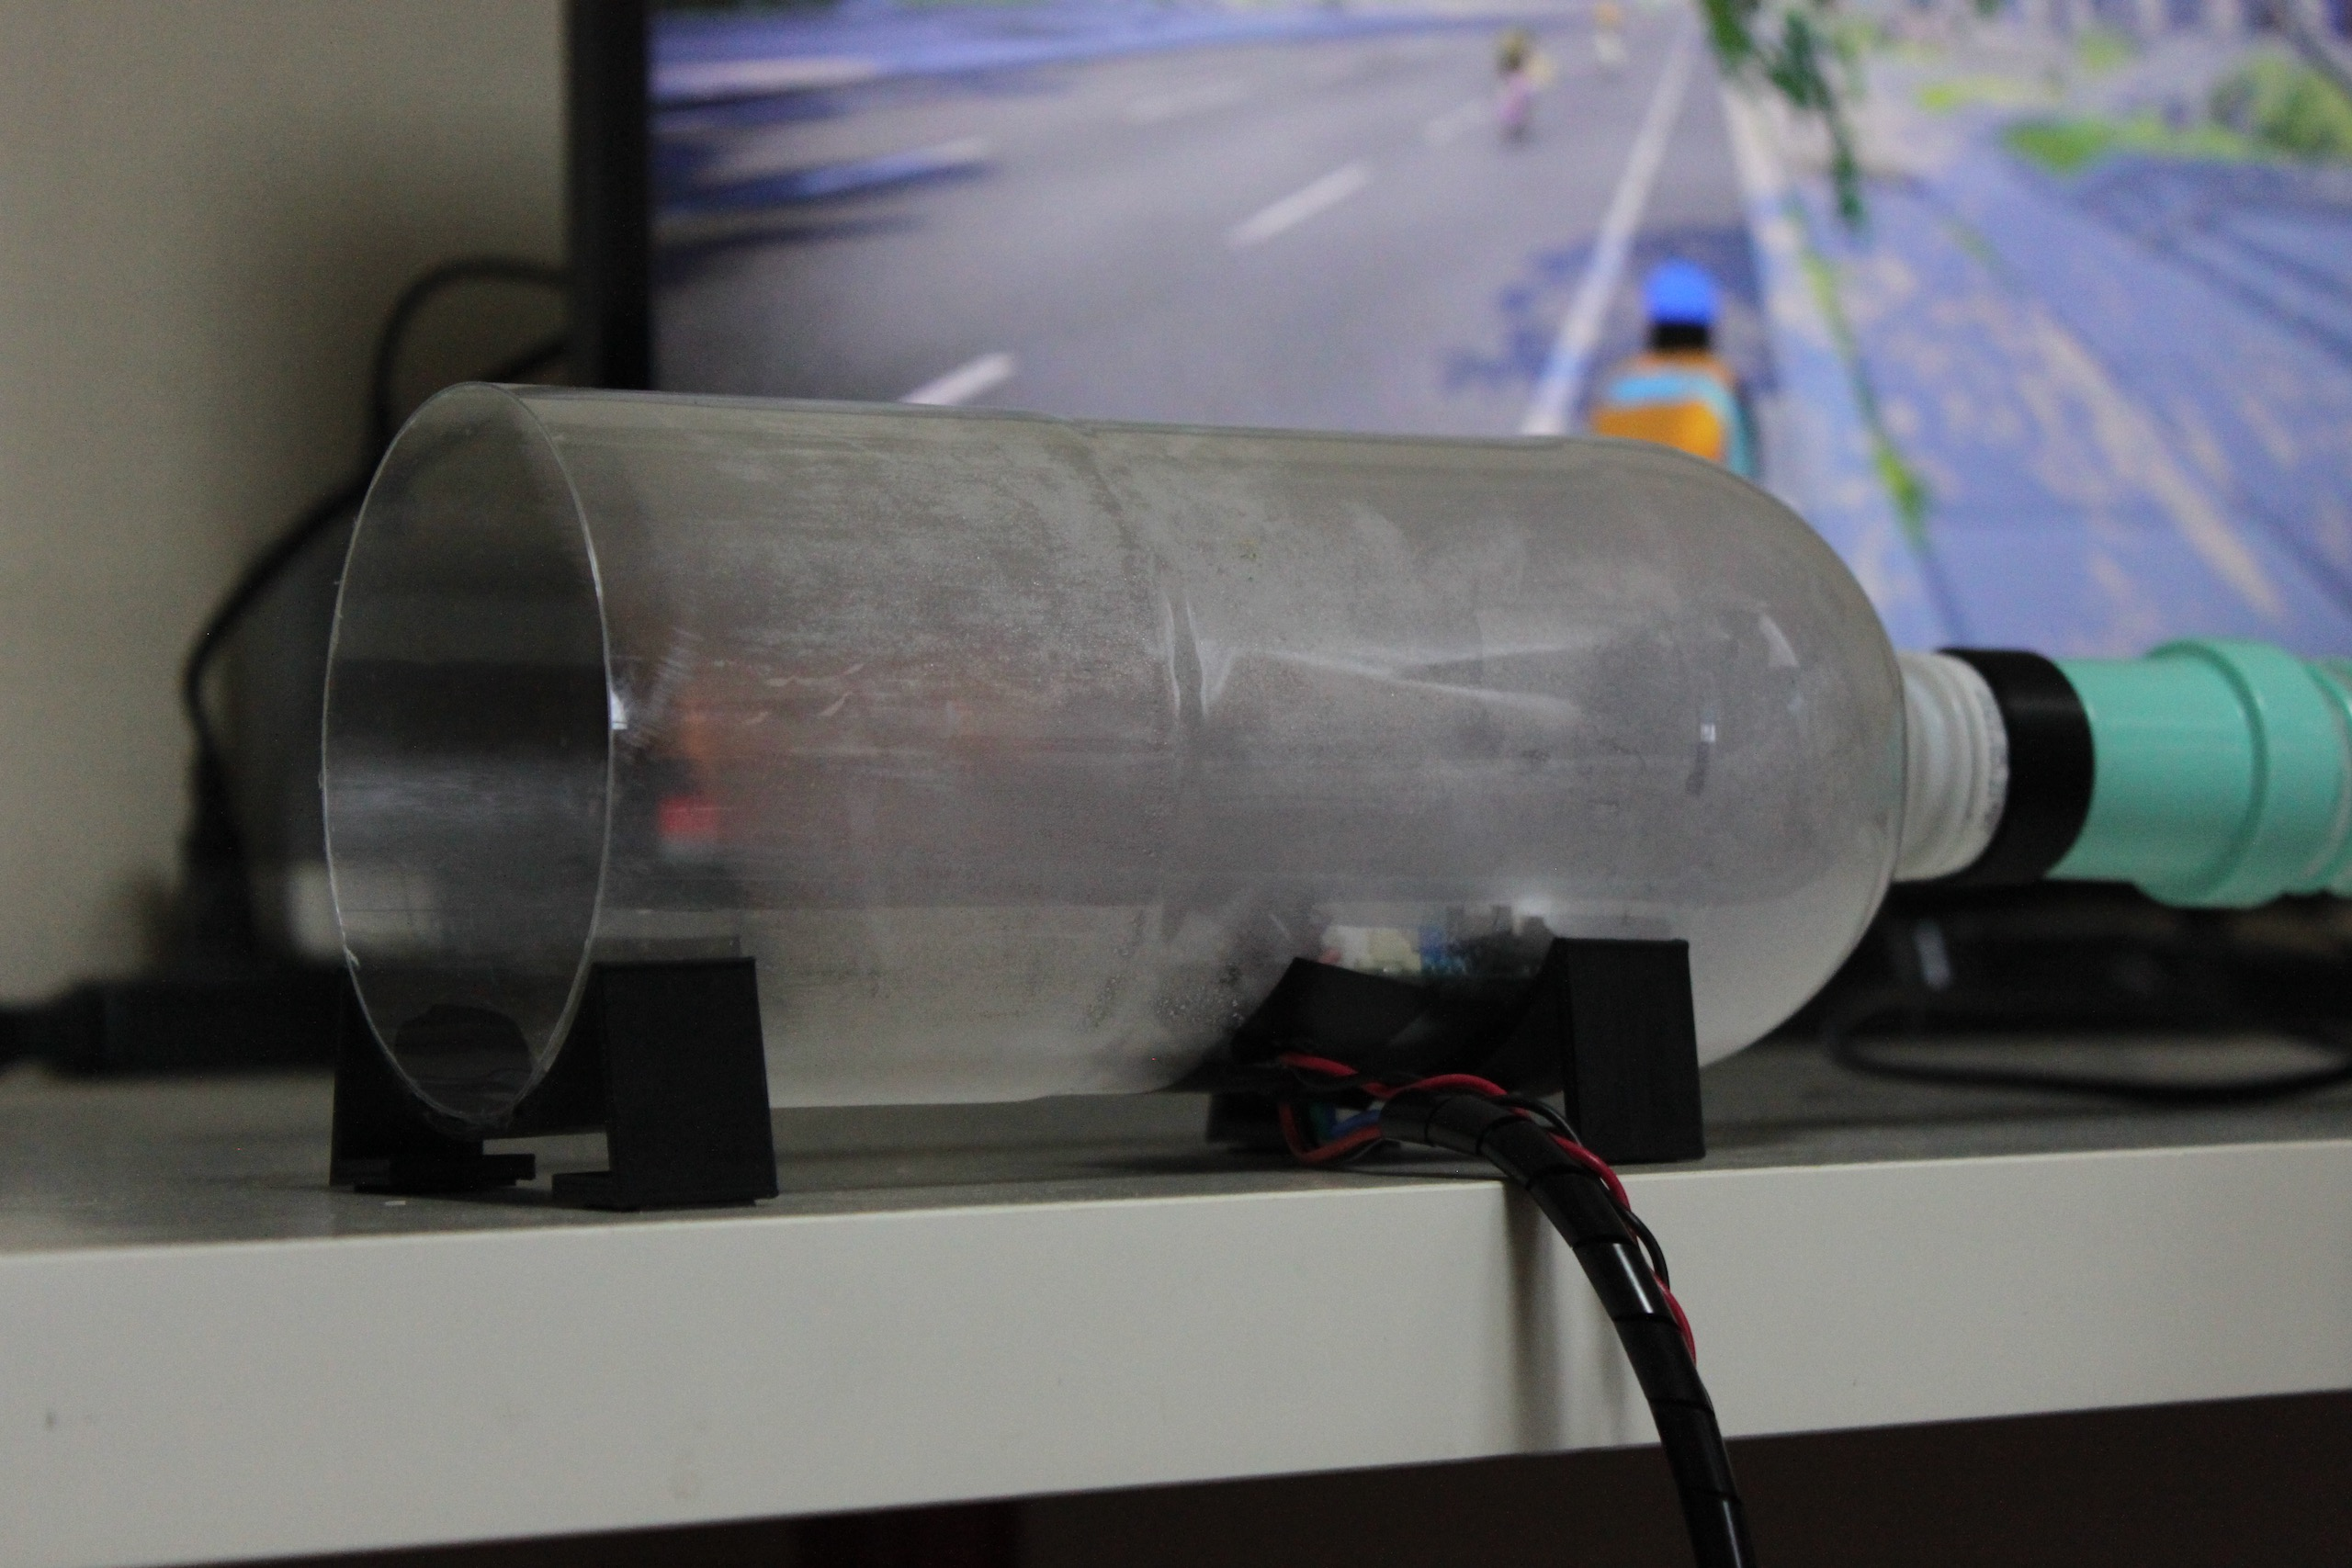
\includegraphics[width=8cm]{fig/mixing_chamber}
    \caption{製作したミキシングチャンバー}
    \label{fig:mixing_chamber}
  \end{center}
\end{figure}

図\ref{fig:mixing_chamber}は今回製作したミキシングチャンバーである.材料には入手のしやすさから,1.5Lの炭酸飲料(CCレモン)のペットボトルを使用した.ミキシングチャンバーとホース(図\ref{fig:hose})を接合するためのジョイント部品はペットボトルのキャップ部のネジをした取り外し式としたものを3Dプリンターで製作した.

当初,ミキシングチャンバーは図\ref{fig:mixing_chamber_early}のように,チャンバー内のガス濃度の変化を小さくすることを意図して,ペットボトルのキャップ部同士を組み合わせて出口の流路を絞った形状としていた.しかし,実際に運動中の測定を行った場合,1分以内でチャンバー内の二酸化炭素濃度がセンサーの測定範囲を超えて上昇してしまうことが分かった.そこで,測定中は極度にガスを溜め込まず,換気を図るためにチャンバー内には特に障害物を設けず,片側を解放した図\ref{fig:mixing_chamber}のような形状とした.

呼気ガスの成分のうち,二酸化炭素は気体標準状態において空気の2倍程度の密度があることから,下方に滞留すると思われる.この際にミキシングチャンバーを置く方向が換気状況に大きく影響を与えることが予想されたので,今回はチャンバーを水平に保った状態で固定することとした.チャンバーとなるペットボトルを水平に保持できるようにするため,スタンド状の部品を3Dプリンターで製作し,センサー側の部品はネジ留めで,もう一方の部品はホットボンドで固定した.

\begin{figure}[H]
  \begin{center}
    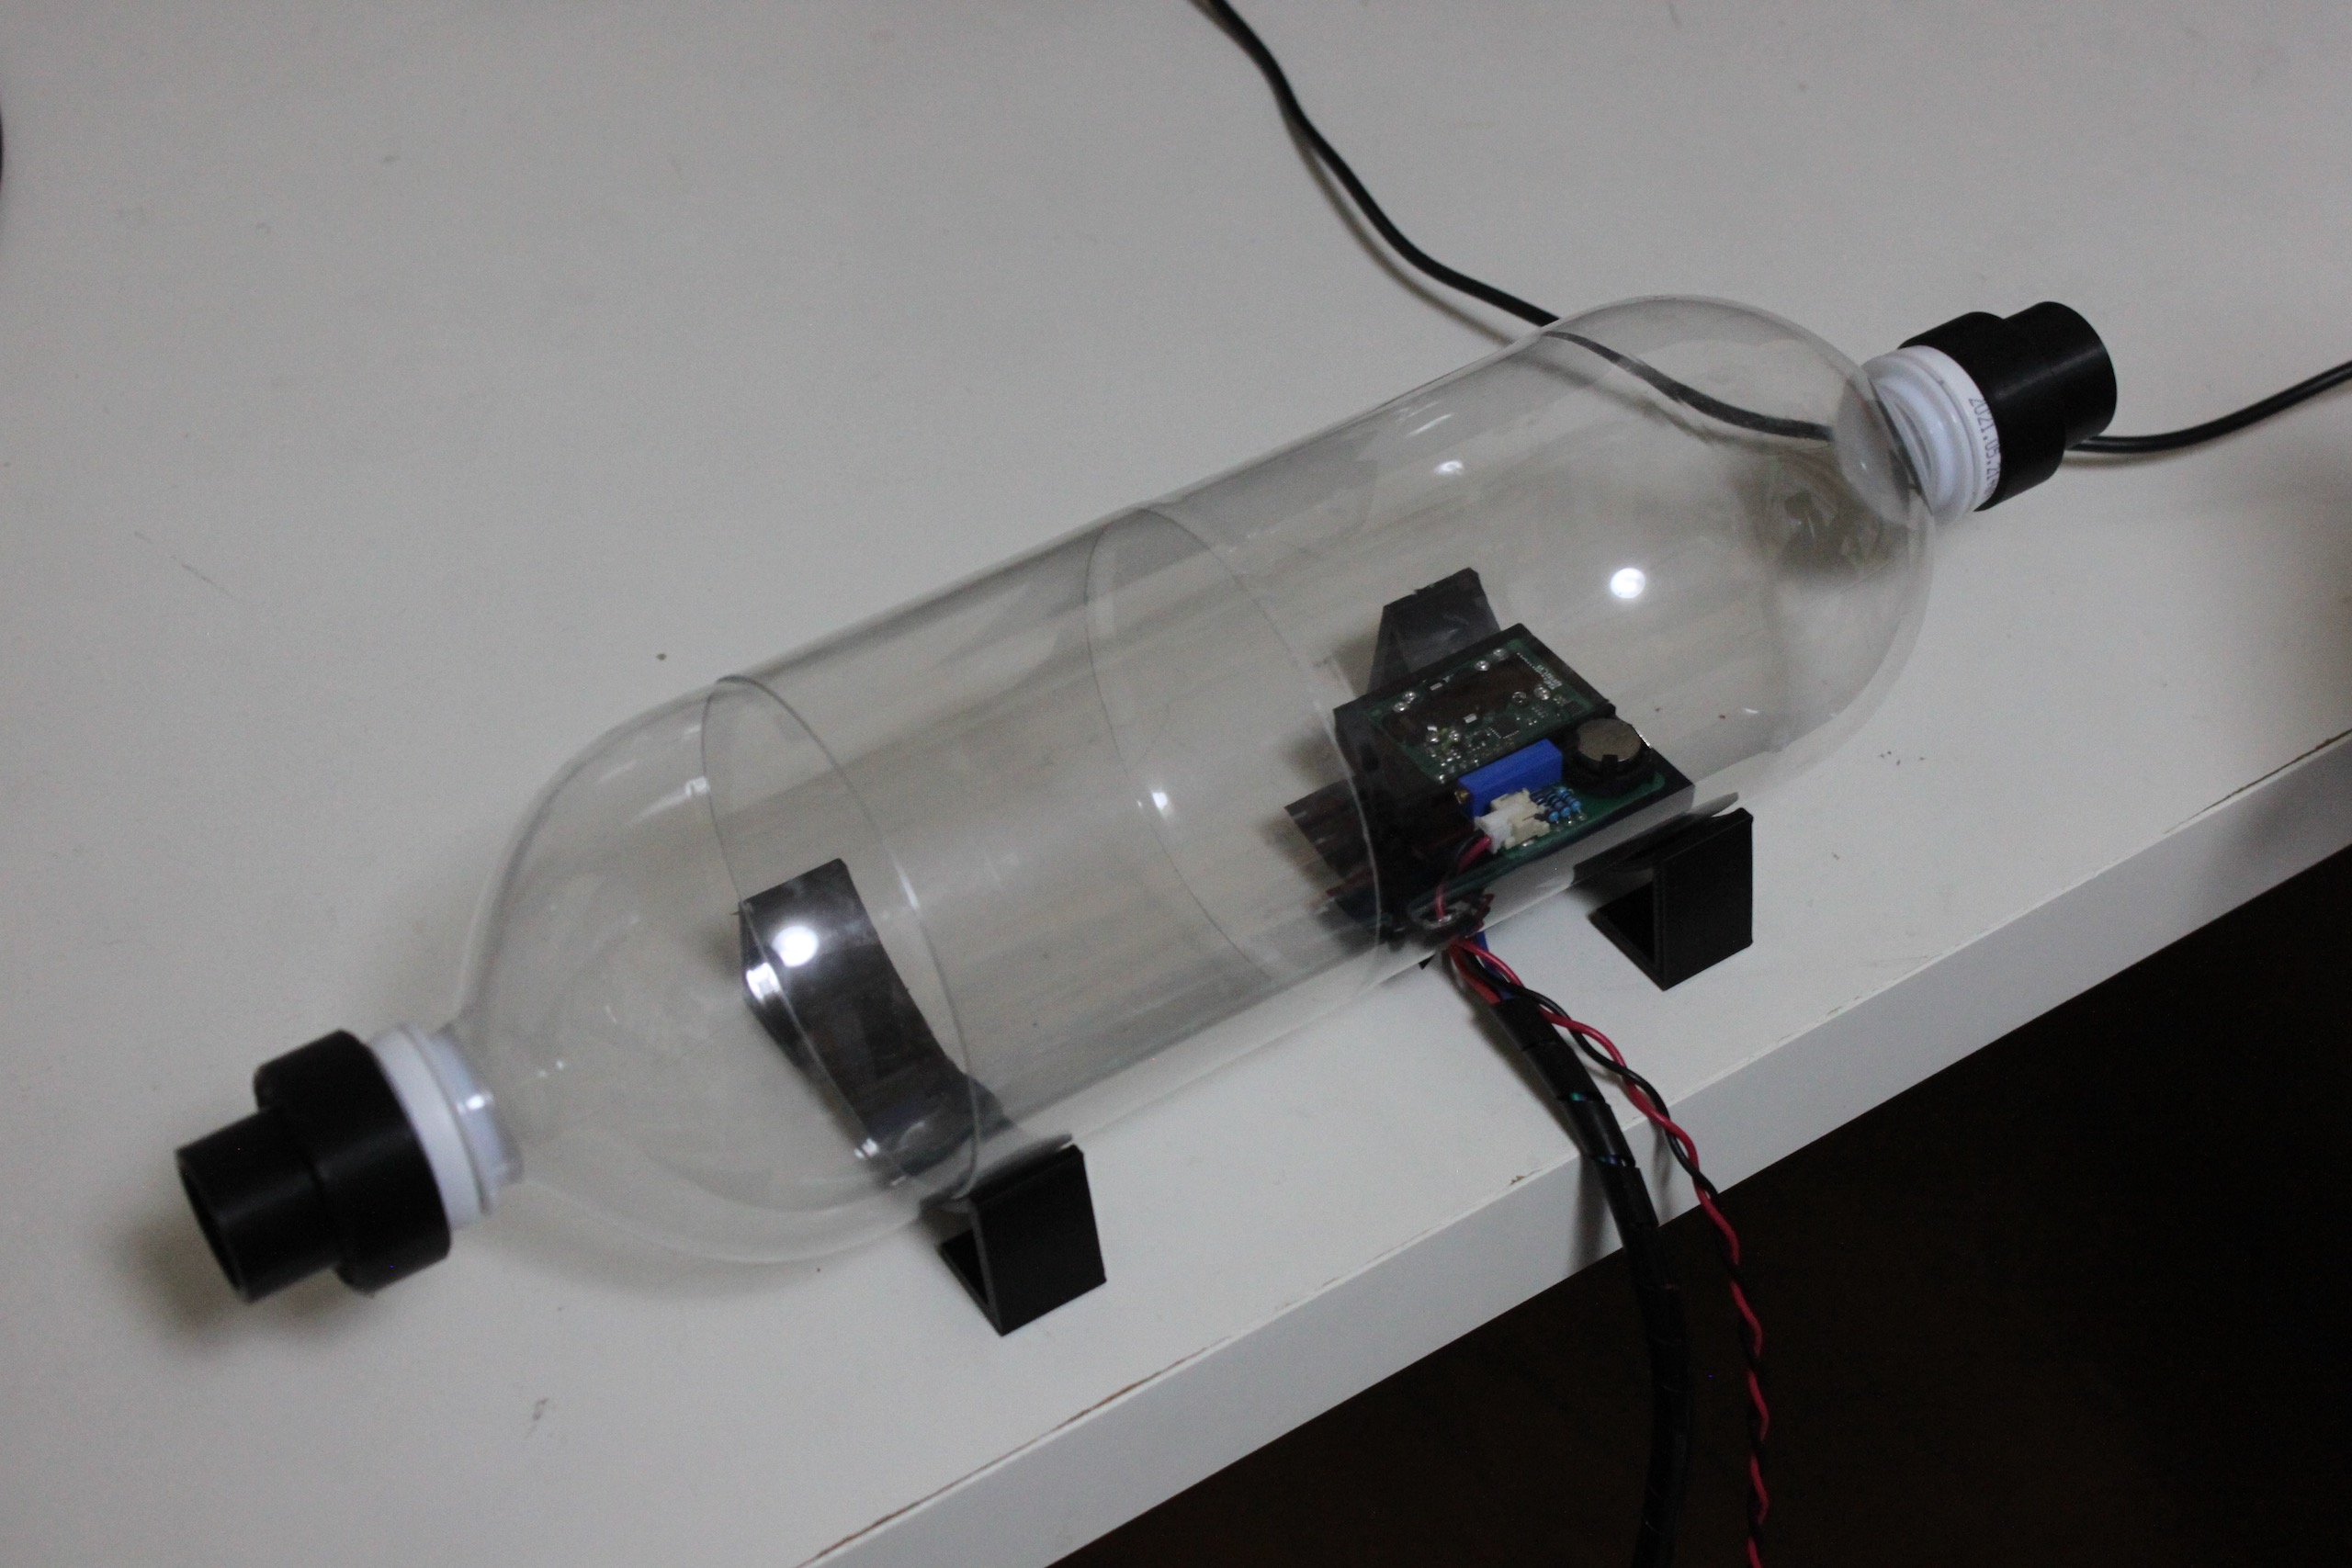
\includegraphics[width=8cm]{fig/mixing_chamber_early}
    \caption{当初のミキシングチャンバー}
    \label{fig:mixing_chamber_early}
  \end{center}
\end{figure}

\subsubsection{呼気収集マスク}

\begin{figure}[H]
  \begin{center}
    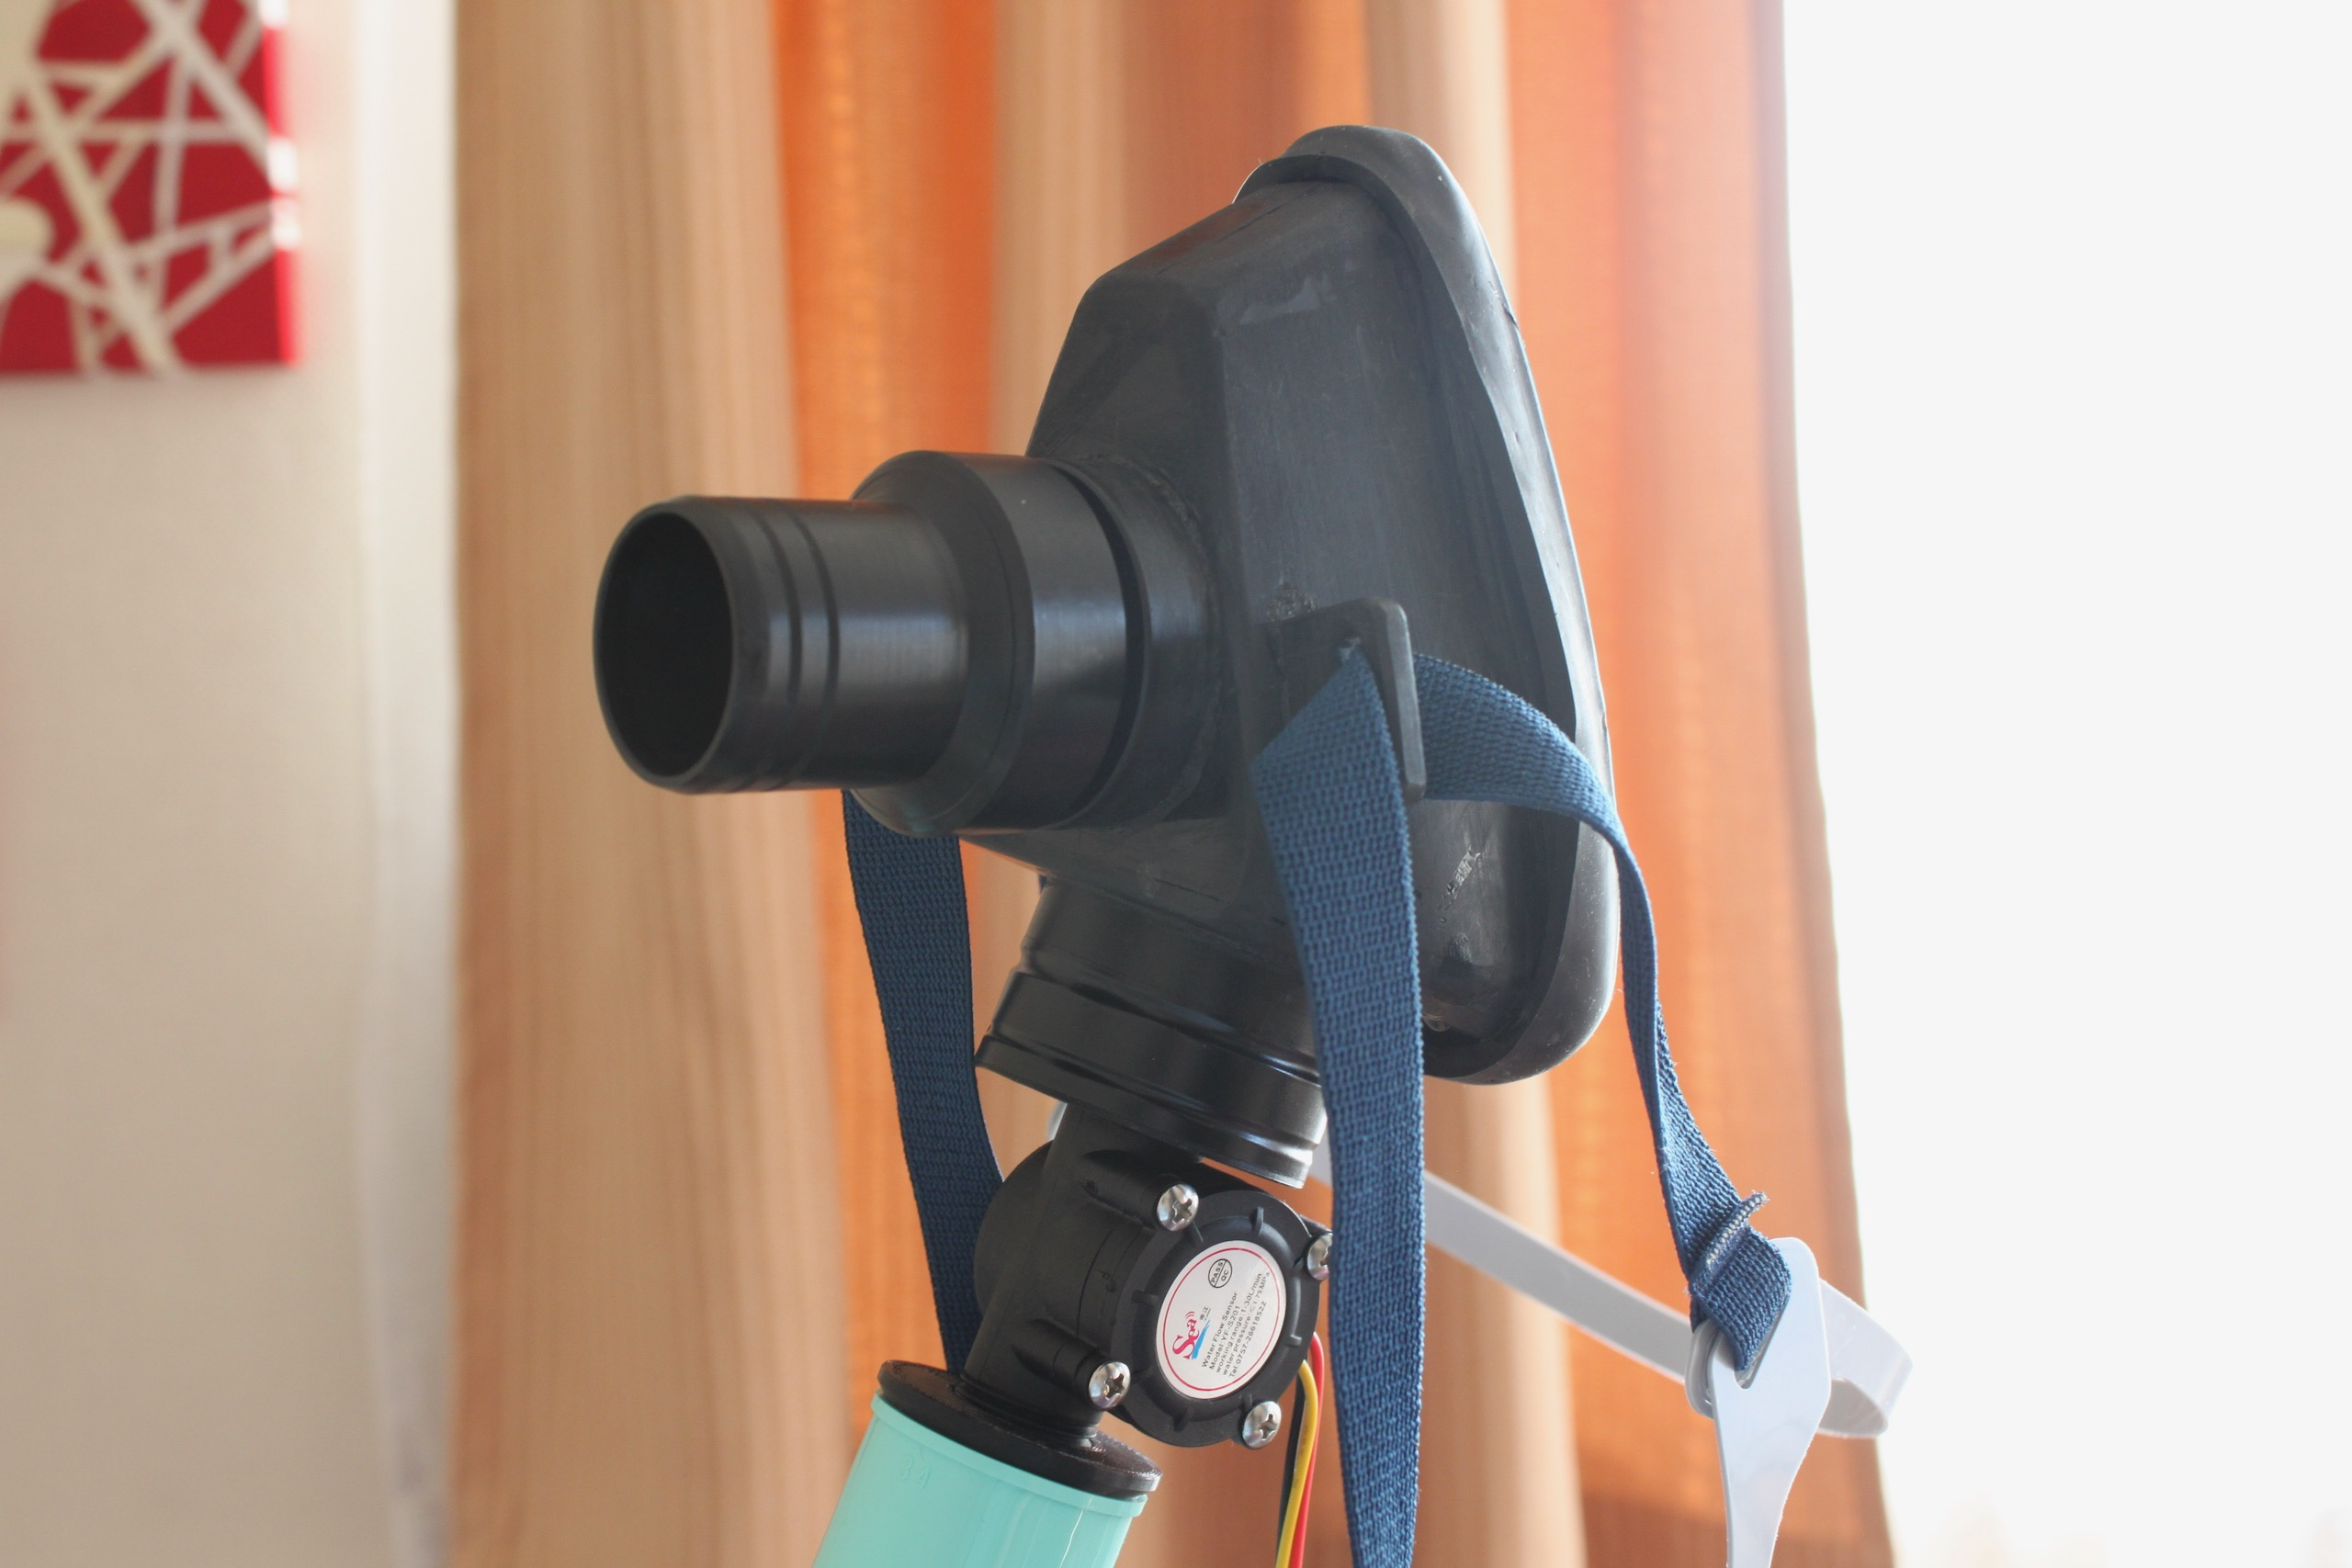
\includegraphics[width=8cm]{fig/mask_front}
    \caption{呼気収集マスク}
    \label{fig:mask_front}
  \end{center}
\end{figure}

呼気を収集するためには,吸気と分離して呼気を収集するためのマスクが必要となる.これをここでは呼気収集マスクと呼ぶことにする.今回は呼気収集マスクには仰木研究室で以前に製作された\cite{mask_build}マスク(図\ref{fig:mask_front})を流用した.これは,樹脂板を組み合わせて顔に合うような形状を構成し,呼気及び吸気用の通気口を取り付けた物である.使用時に両手が使えるように,頭に固定するための市販のガスマスクから流用したバンドが取り付けられている.マスクの内側の顔に触れる部分には,顔との間にできる隙間を埋め呼気ガスが呼気の通気口以外から漏れ出すことを防ぐためのパッドが取り付けられている(\ref{fig:mask_rear}).このパッドは超伸縮機能を有する山本化学工業のバイオラバー素材によって作られている.

\begin{figure}[H]
  \begin{center}
    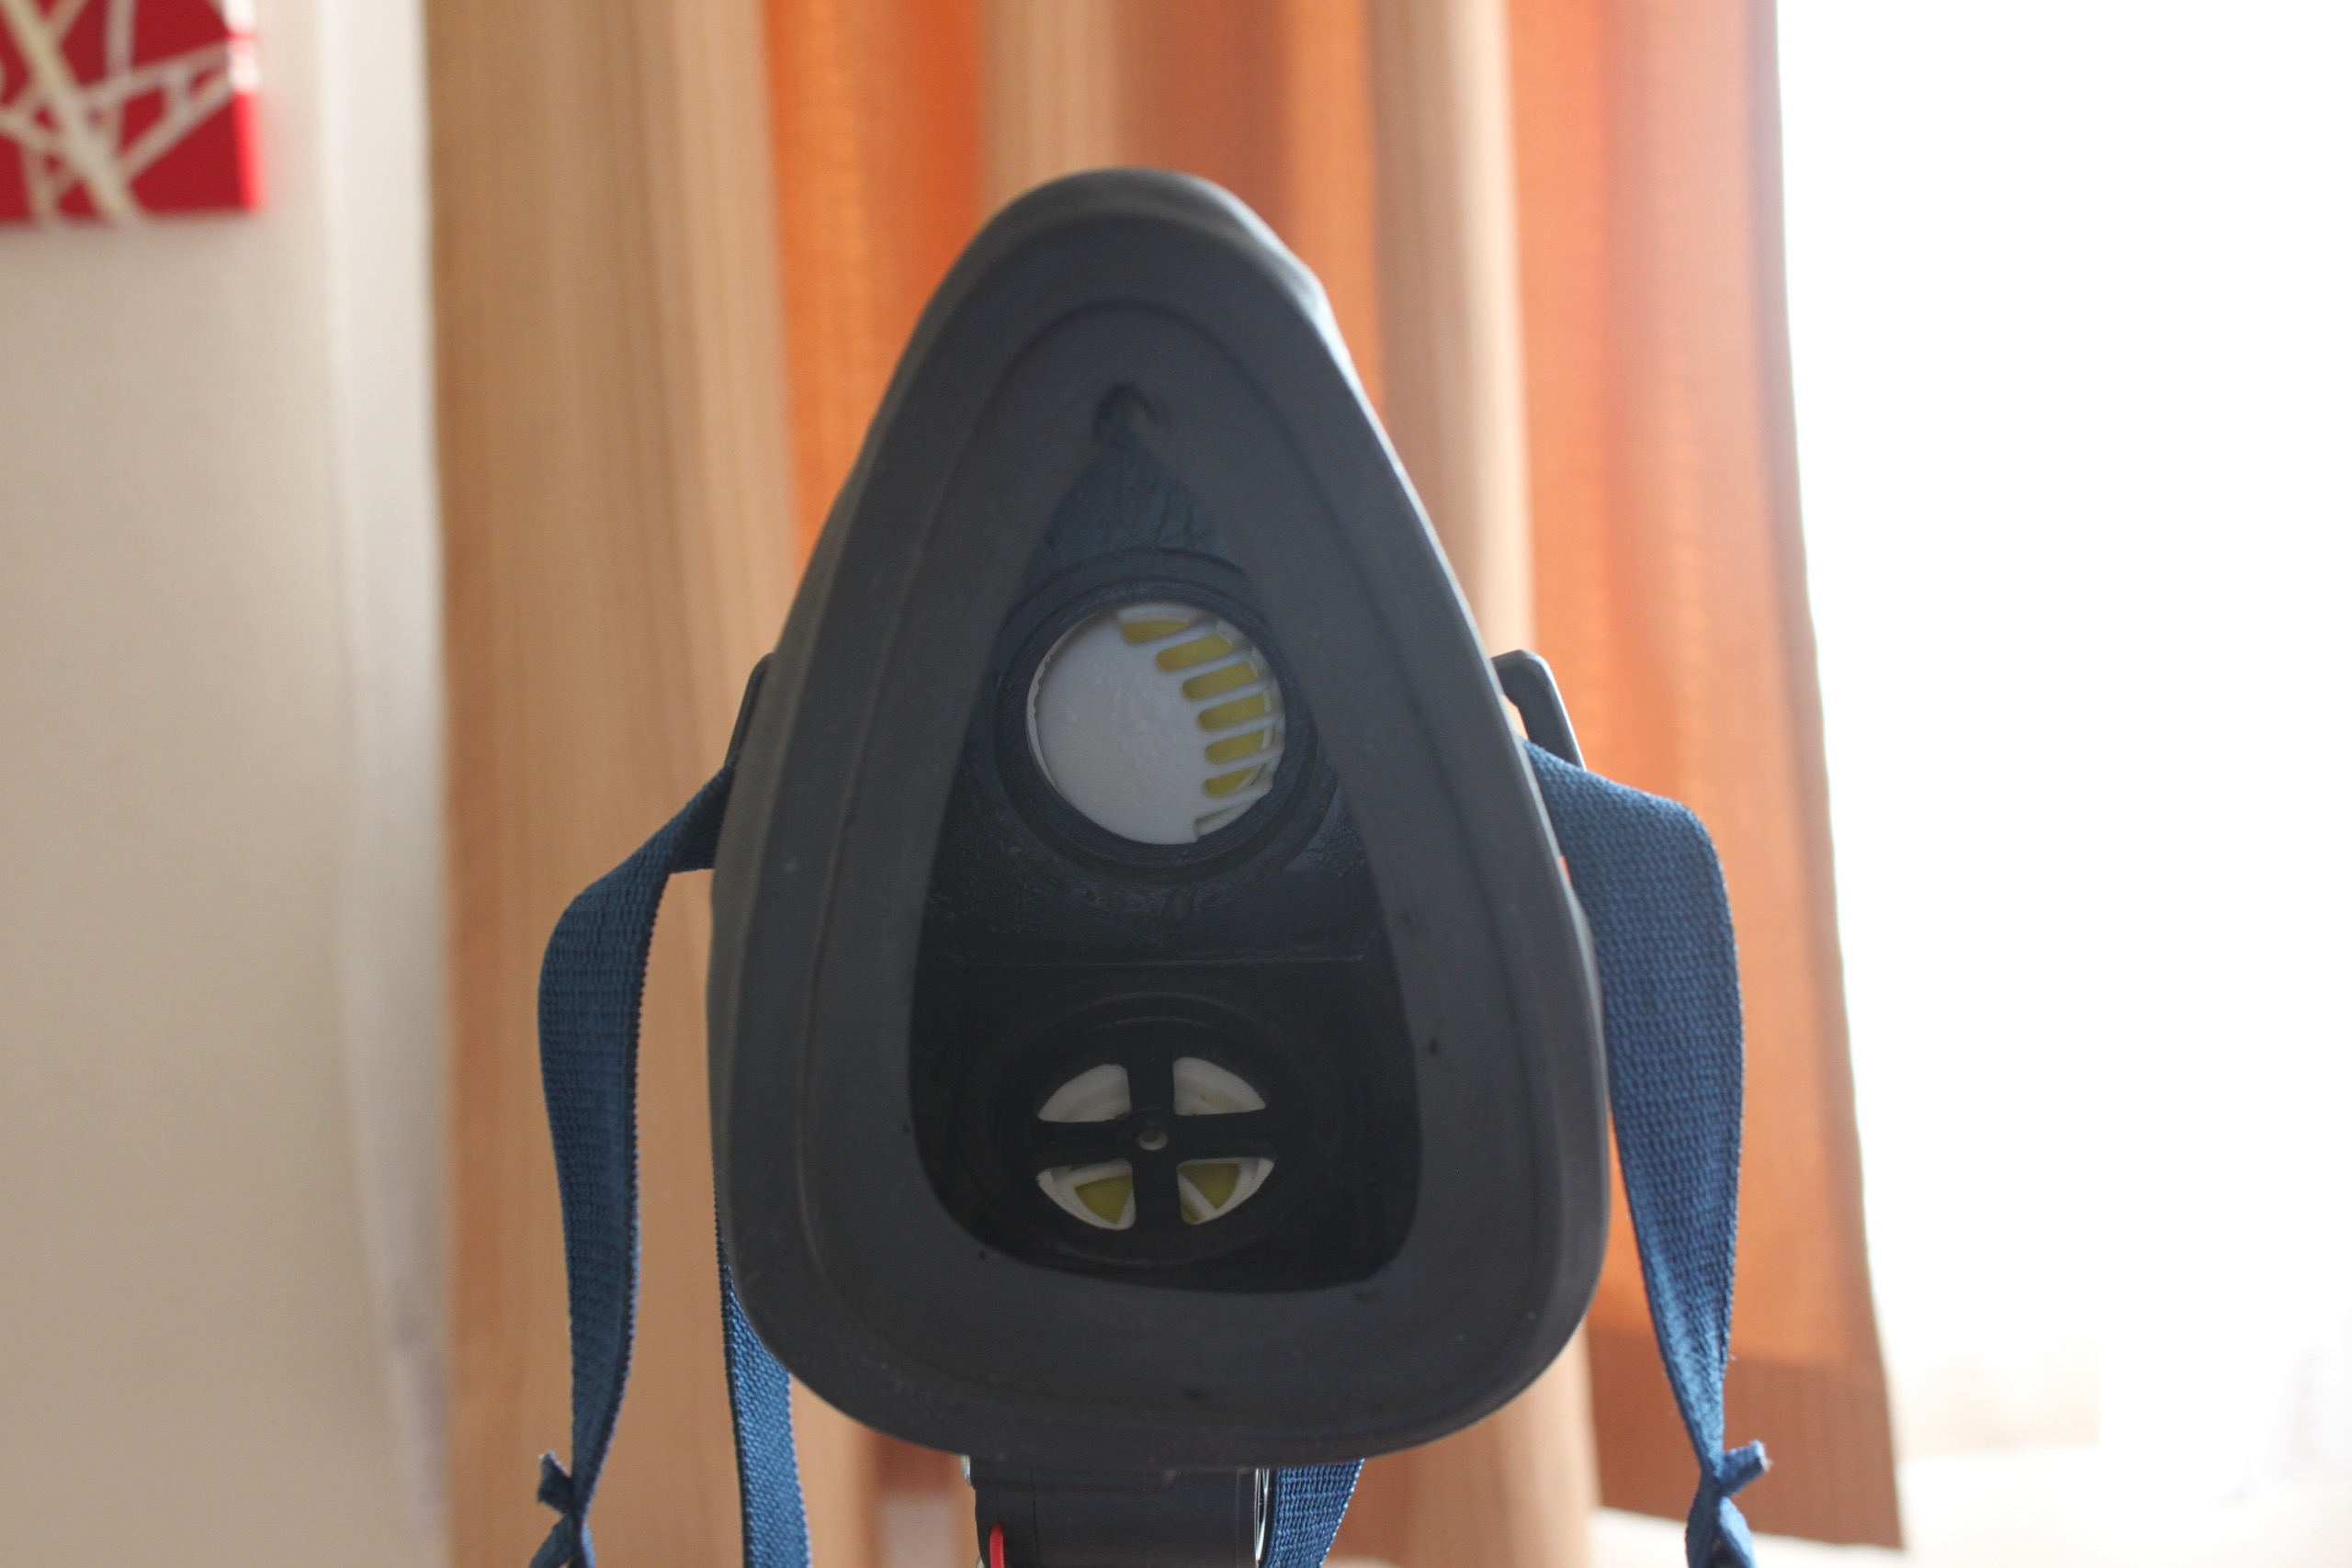
\includegraphics[width=8cm]{fig/mask_rear}
    \caption{内側から見た呼気収集マスク}
    \label{fig:mask_rear}
  \end{center}
\end{figure}

マスクの内側には,吸気と呼気を分離するために逆流防止弁を取り付けた(図\ref{fig:mask_rear}).なお,一般的なガスマスクに倣い,今回は鼻の前あたりに位置する前方向の通気口を吸気,口の前下あたりに位置する下方向の通気口を呼気とした.今回使用した逆流防止弁は,運動時に使用するマスクに取り付けるために安価に市販されている物である.逆流防止弁の構造は図\ref{fig:bulb}のようになっている.ごく薄いシリコーンゴム製の膜は,一方向のみに捲れることができるようにプラスチック製の2つのパーツに挟まれて取り付けられている.これによって,弁を流れる気体の流れる方向を一方向に制限することができる.この弁を3Dプリンターで製作したスペーサーでマスク本体の径に合わせた上でネジで固定している.

\begin{figure}[H]
  \begin{center}
    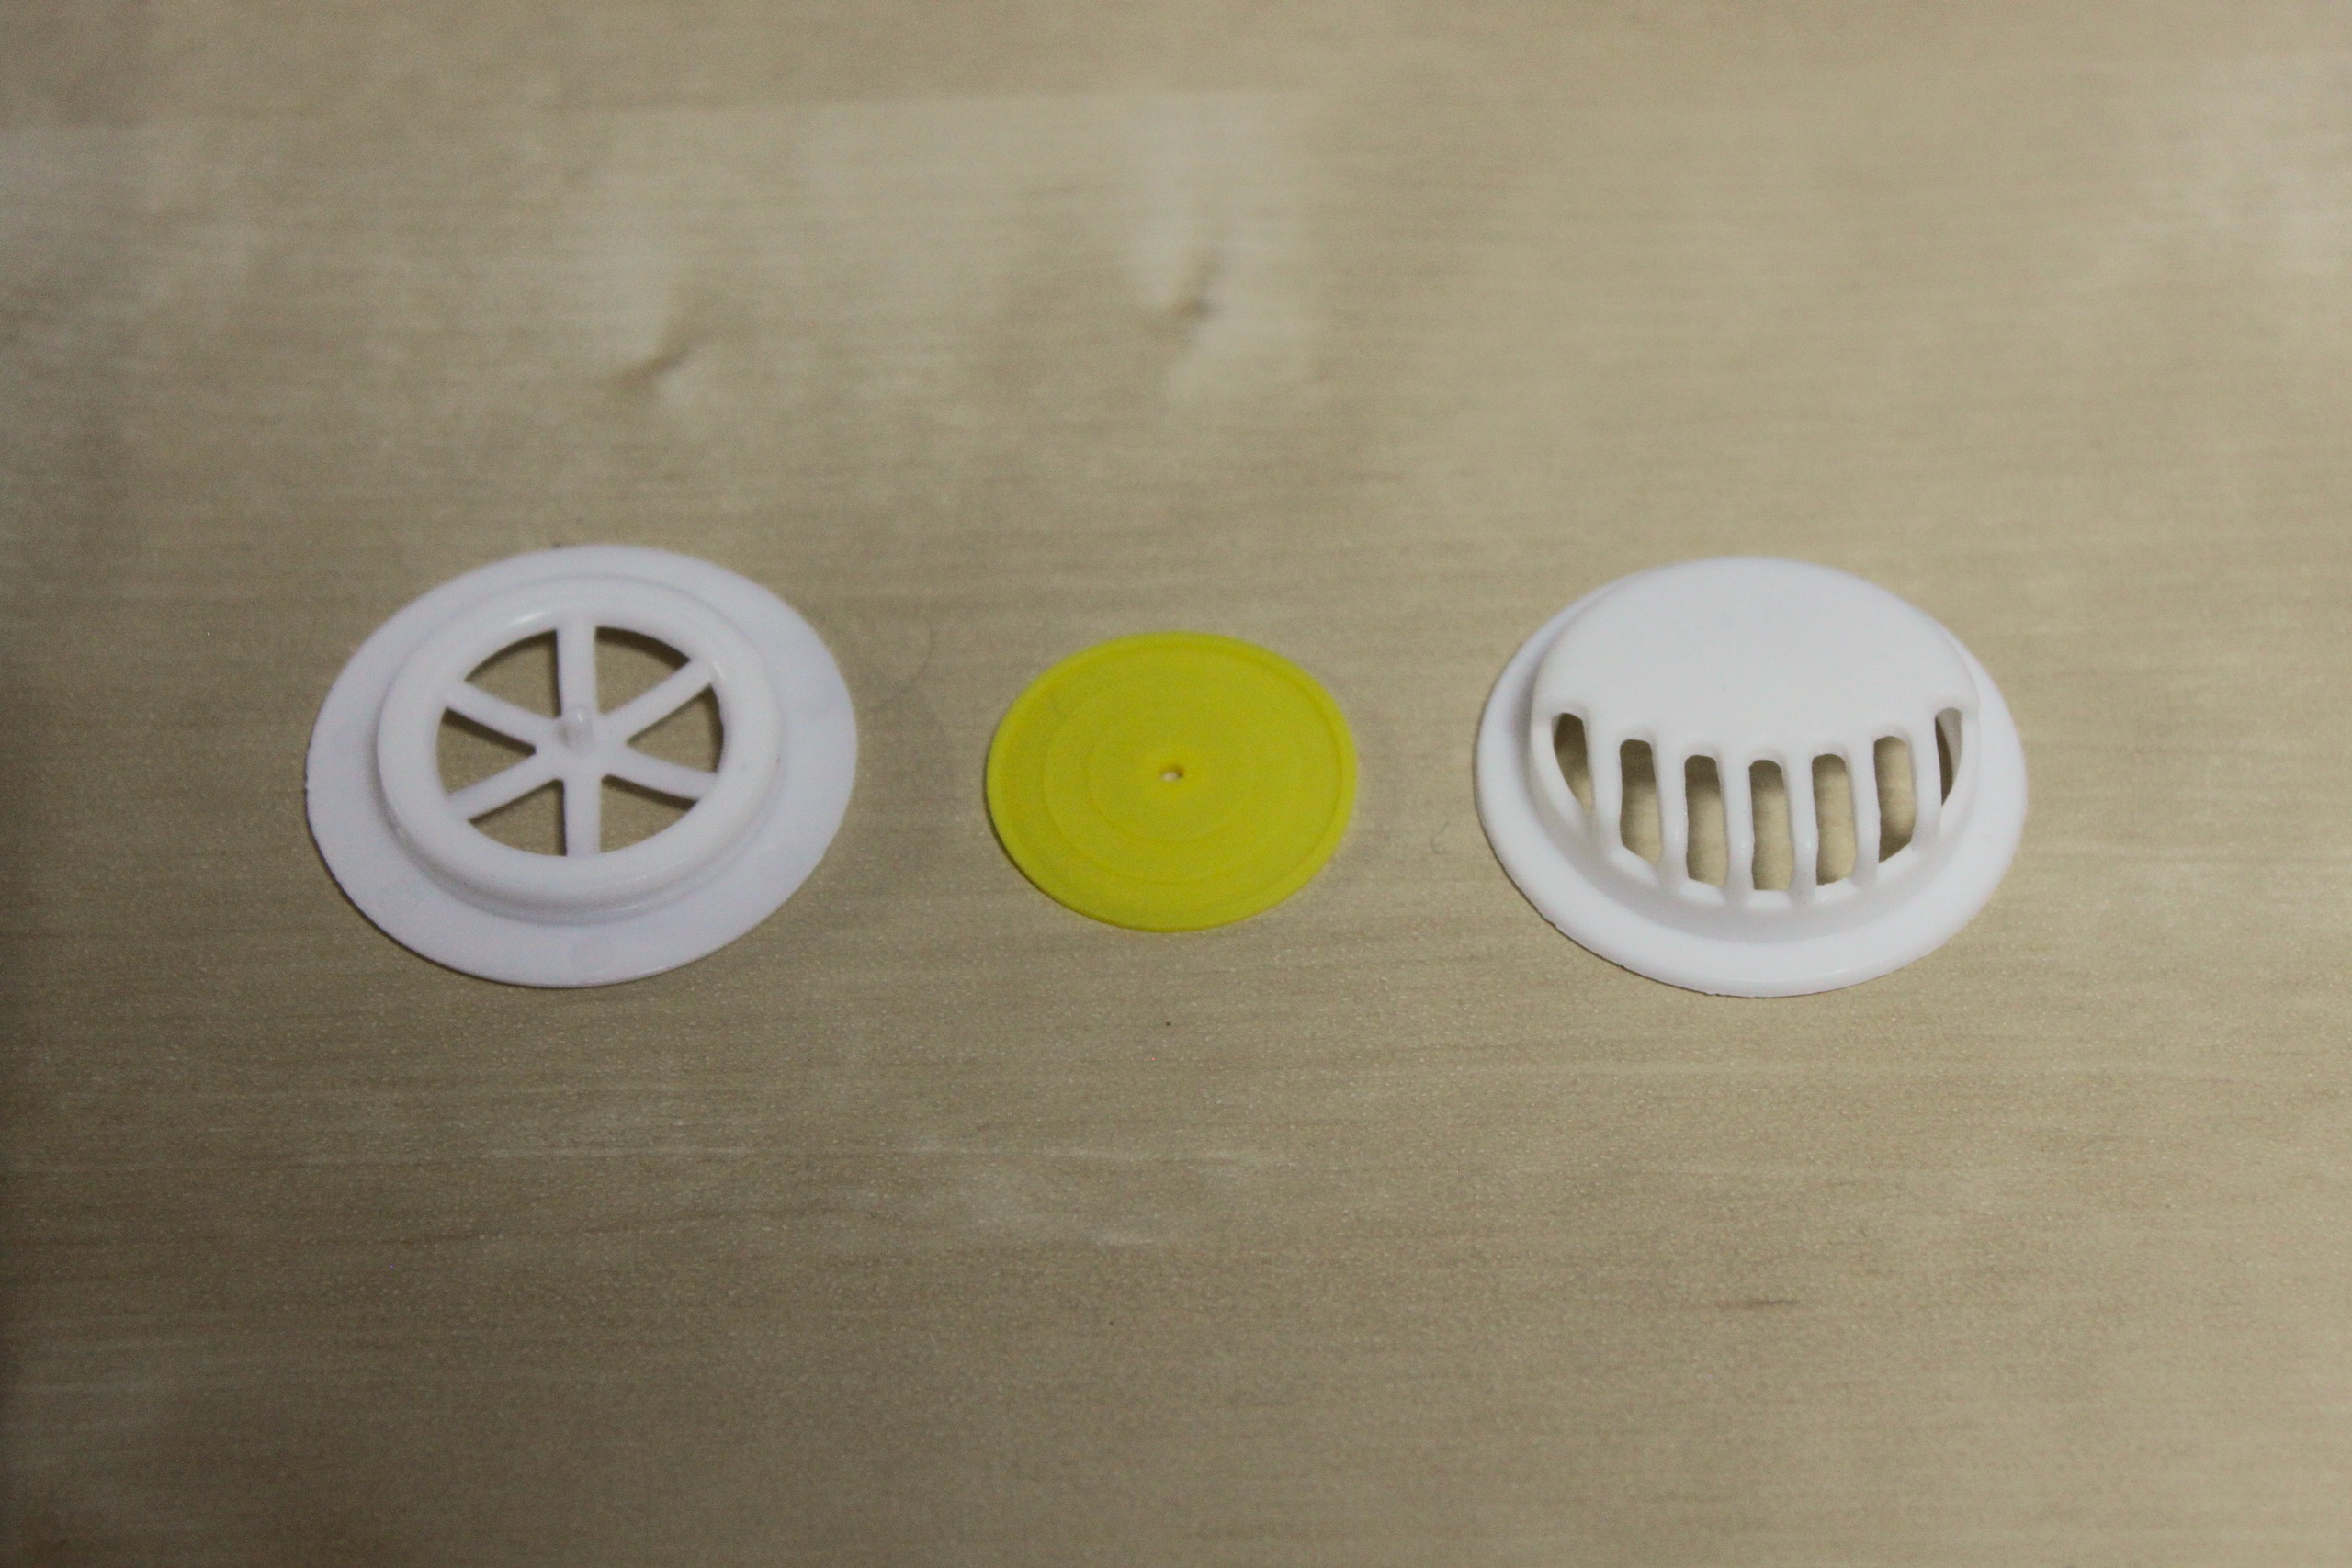
\includegraphics[width=8cm]{fig/bulb}
    \caption{逆流防止弁の構造}
    \label{fig:bulb}
  \end{center}
\end{figure}

ミキシングチャンバーと呼気収集マスクを接続するためのホースには,洗濯機の排水用ホースの延長用として市販されている物(図\ref{fig:hose})を使用した.このホースは内径30mmの塩化ビニル製で,片側がゴム製,もう片側が硬質プラスチック製の継手となっている.今回はチャンバー側にプラスチック製,マスク側にゴム製の継手を接続することにし,ジョイント部品を3Dプリンターで製作した.

\begin{figure}[H]
  \begin{center}
    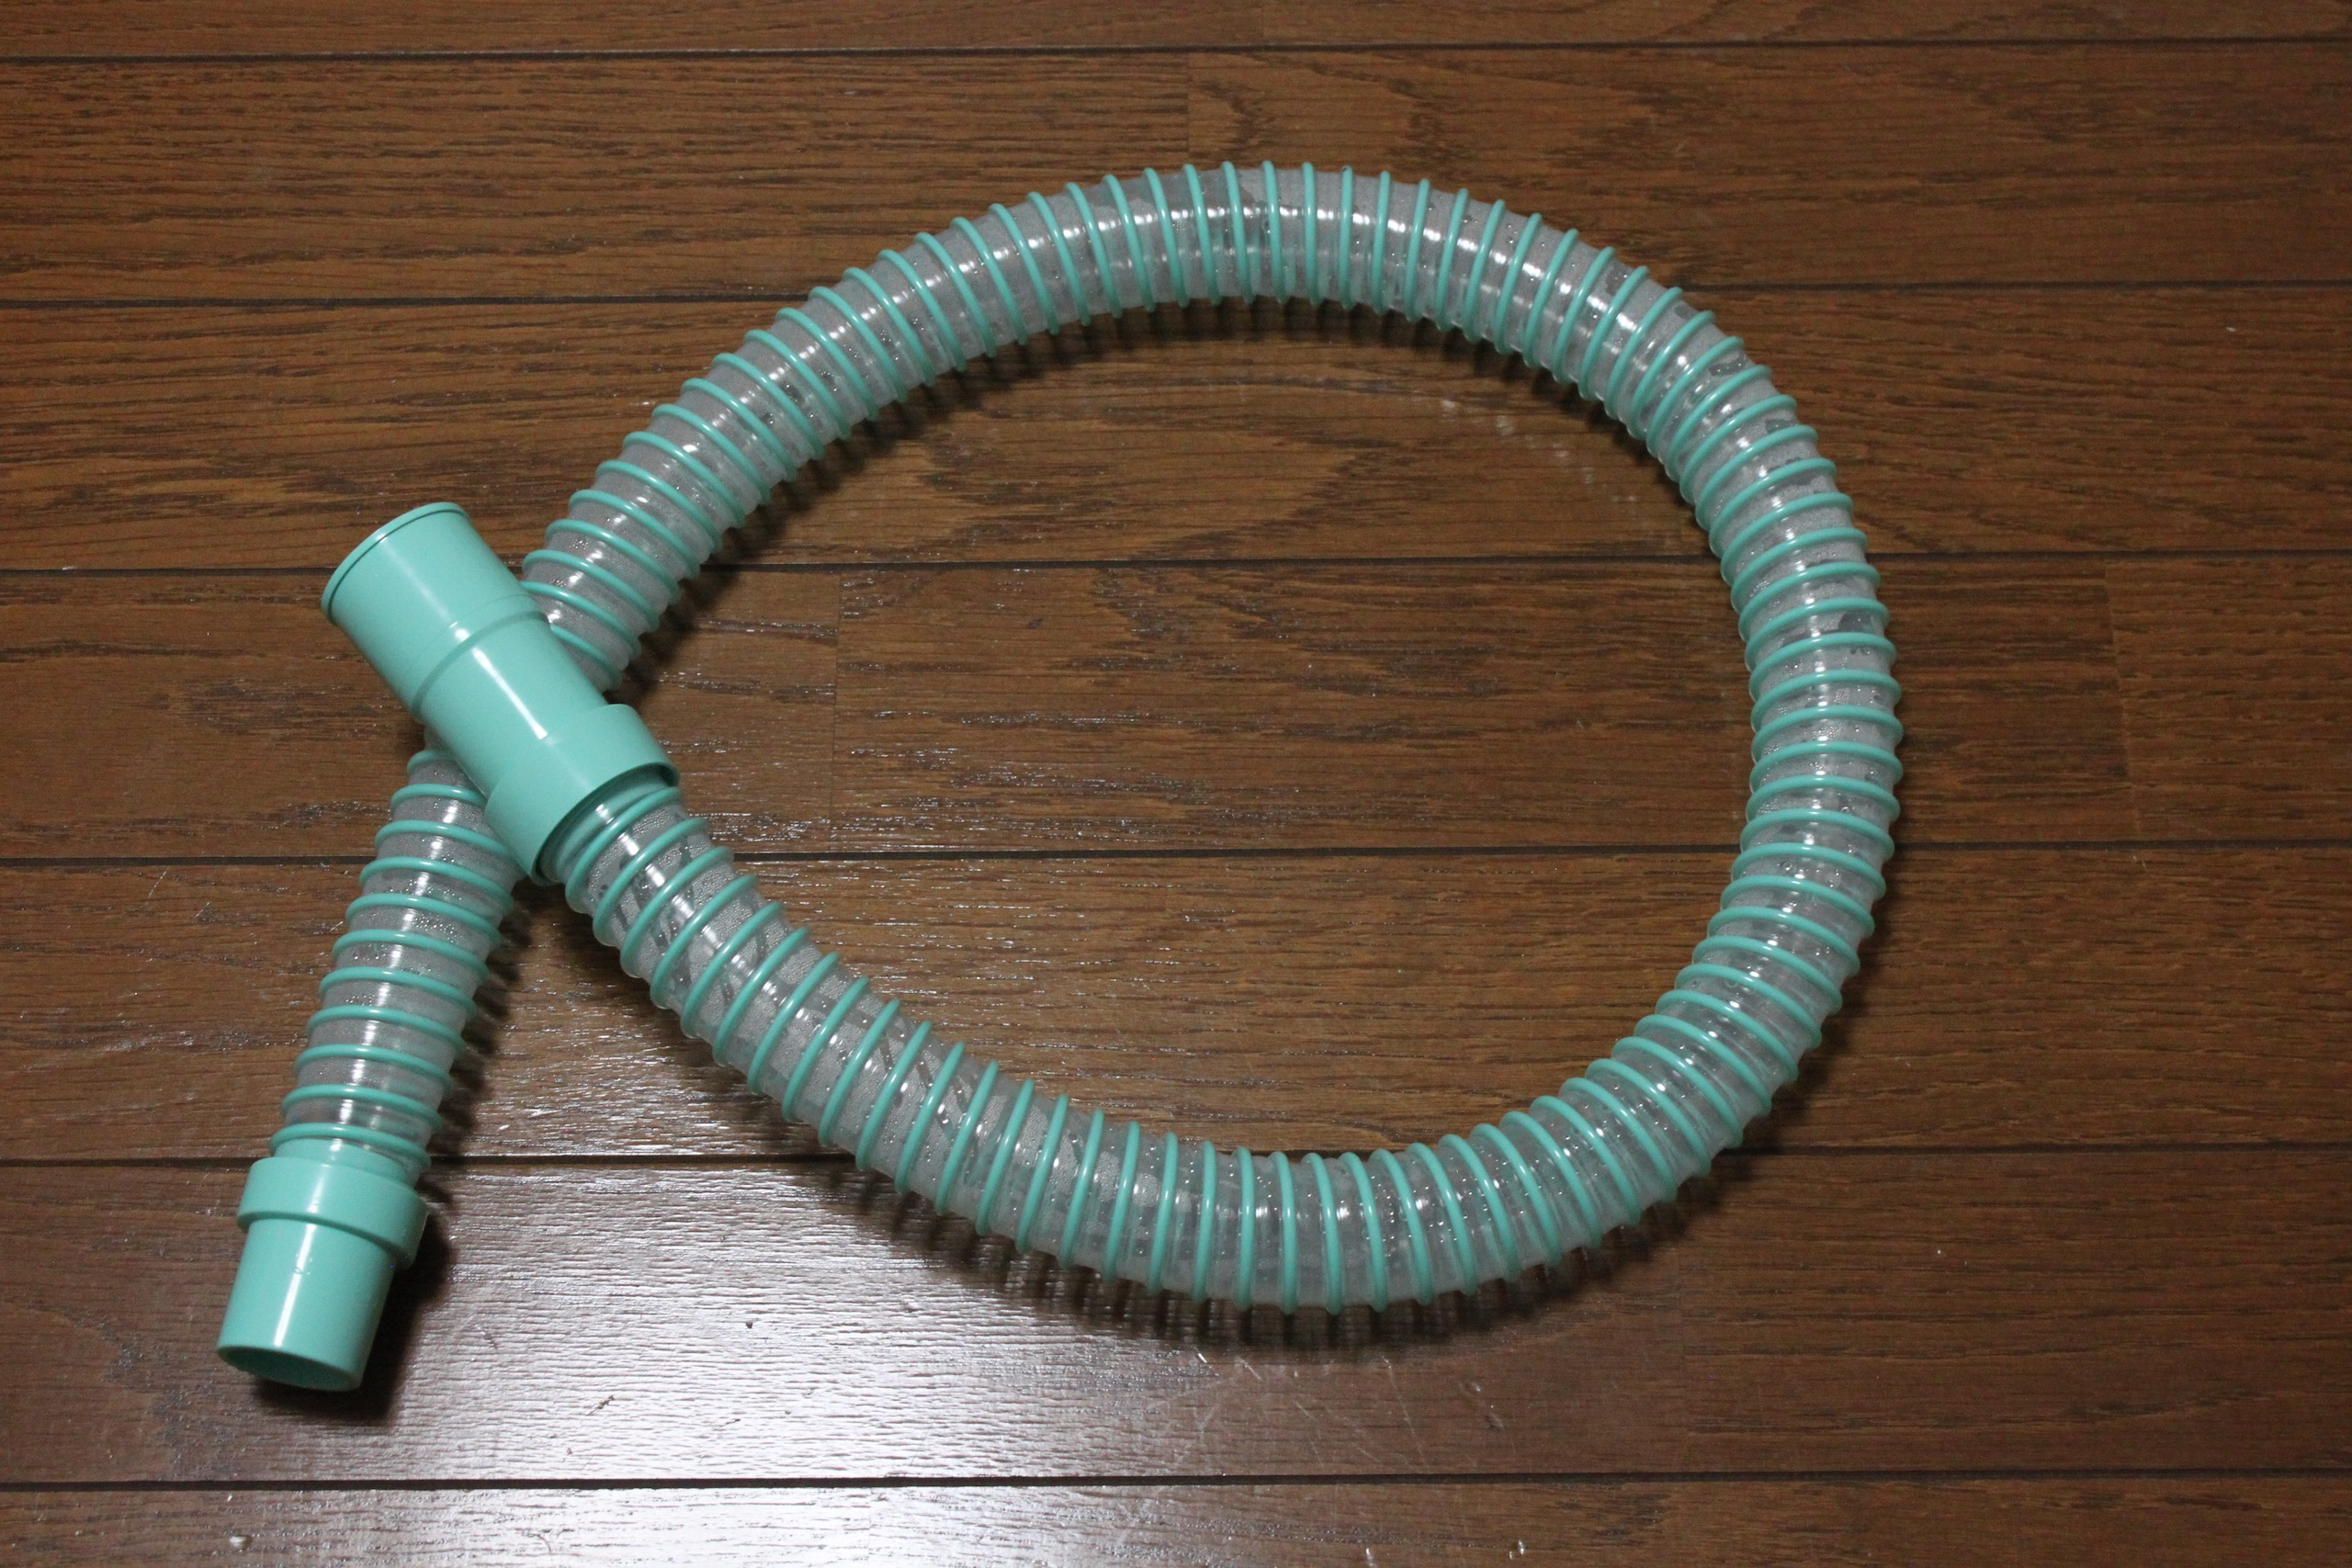
\includegraphics[width=8cm]{fig/hose}
    \caption{洗濯ホース}
    \label{fig:hose}
  \end{center}
\end{figure}

\subsection{換気量の測定}

\subsubsection{計測方式}

\ref{sec:correct}に述べたように,今回はミキシングチャンバー方式で呼気を収集する.ミキシングチャンバー法では,換気量の測定を呼気の流路に流量計を設置することで収集中に行う必要がある.

気体の流量を測定するための流量計の原理としては,差圧流量計と超音波流量計,タービン流量計などがある.各方式の特徴を表\ref{tb:flowsensor_method}にまとめた.

\begin{table}[H]
\begin{center}
\caption{主な気体流量計の測定方式}
\label{tb:flowsensor_method}
\begin{tabular}{|l|l|l|}
\hline
 & 原理 & 構造 \\ \hline
差圧流量計   & \begin{tabular}[c]{@{}l@{}}流路内に流路を絞った機構を設ける.\\ その前後に発生する圧力差を測定する.\end{tabular}    & 微細     \\ \hline
超音波流量計  & \begin{tabular}[c]{@{}l@{}}流路内の液体に超音波を照射する.\\ 照射した超音波の反射によって流量を測定する.\end{tabular} & 微細     \\ \hline
タービン流量計 & \begin{tabular}[c]{@{}l@{}}流路内にタービンを設置する.\\ タービンの回転数によって流量を測定する.\end{tabular}     & 微細ではない \\ \hline
\end{tabular}
\end{center}
\end{table}

差圧流量計は流路内に絞り機構を設け,その前後に発生する圧力差を測ることで流量を計測する方式である.超音波流量計は,流路内を流れる流体に超音波を照射することで流量を計測する方式である.タービン流量計は,流路にタービンを設置し,流体によって回転するタービンの回転数によって流量を計測する方式である.

気体流量計はいずれの方式も高価な部品である.呼吸代謝測定装置の製作において,流量計のコストを抑えることは大きな課題であると言える.タービン流量計は単純な構造であり,他の方式に比べて微細ではない構造なので,水流計として安価に市販されている.今回は研究の趣旨として,呼吸代謝測定装置としての性能を多少損なったとしても,装置全体の全体の価格を抑えることを優先し,流量計として水流計を使用した.

今回使用した水流計はYF-S201という名称で市販されているもので,流路に対してタービンの軸が垂直に取り付けられている接線流羽根車式のタービン流量計である.タービンの回転数に応じてホール素子が矩形波の信号を出力する.YF-S201と主な仕様を図\ref{fig:yf-s201}と表\ref{tb:YFS201_specsheet}に示す.

\begin{figure}[H]
  \begin{center}
    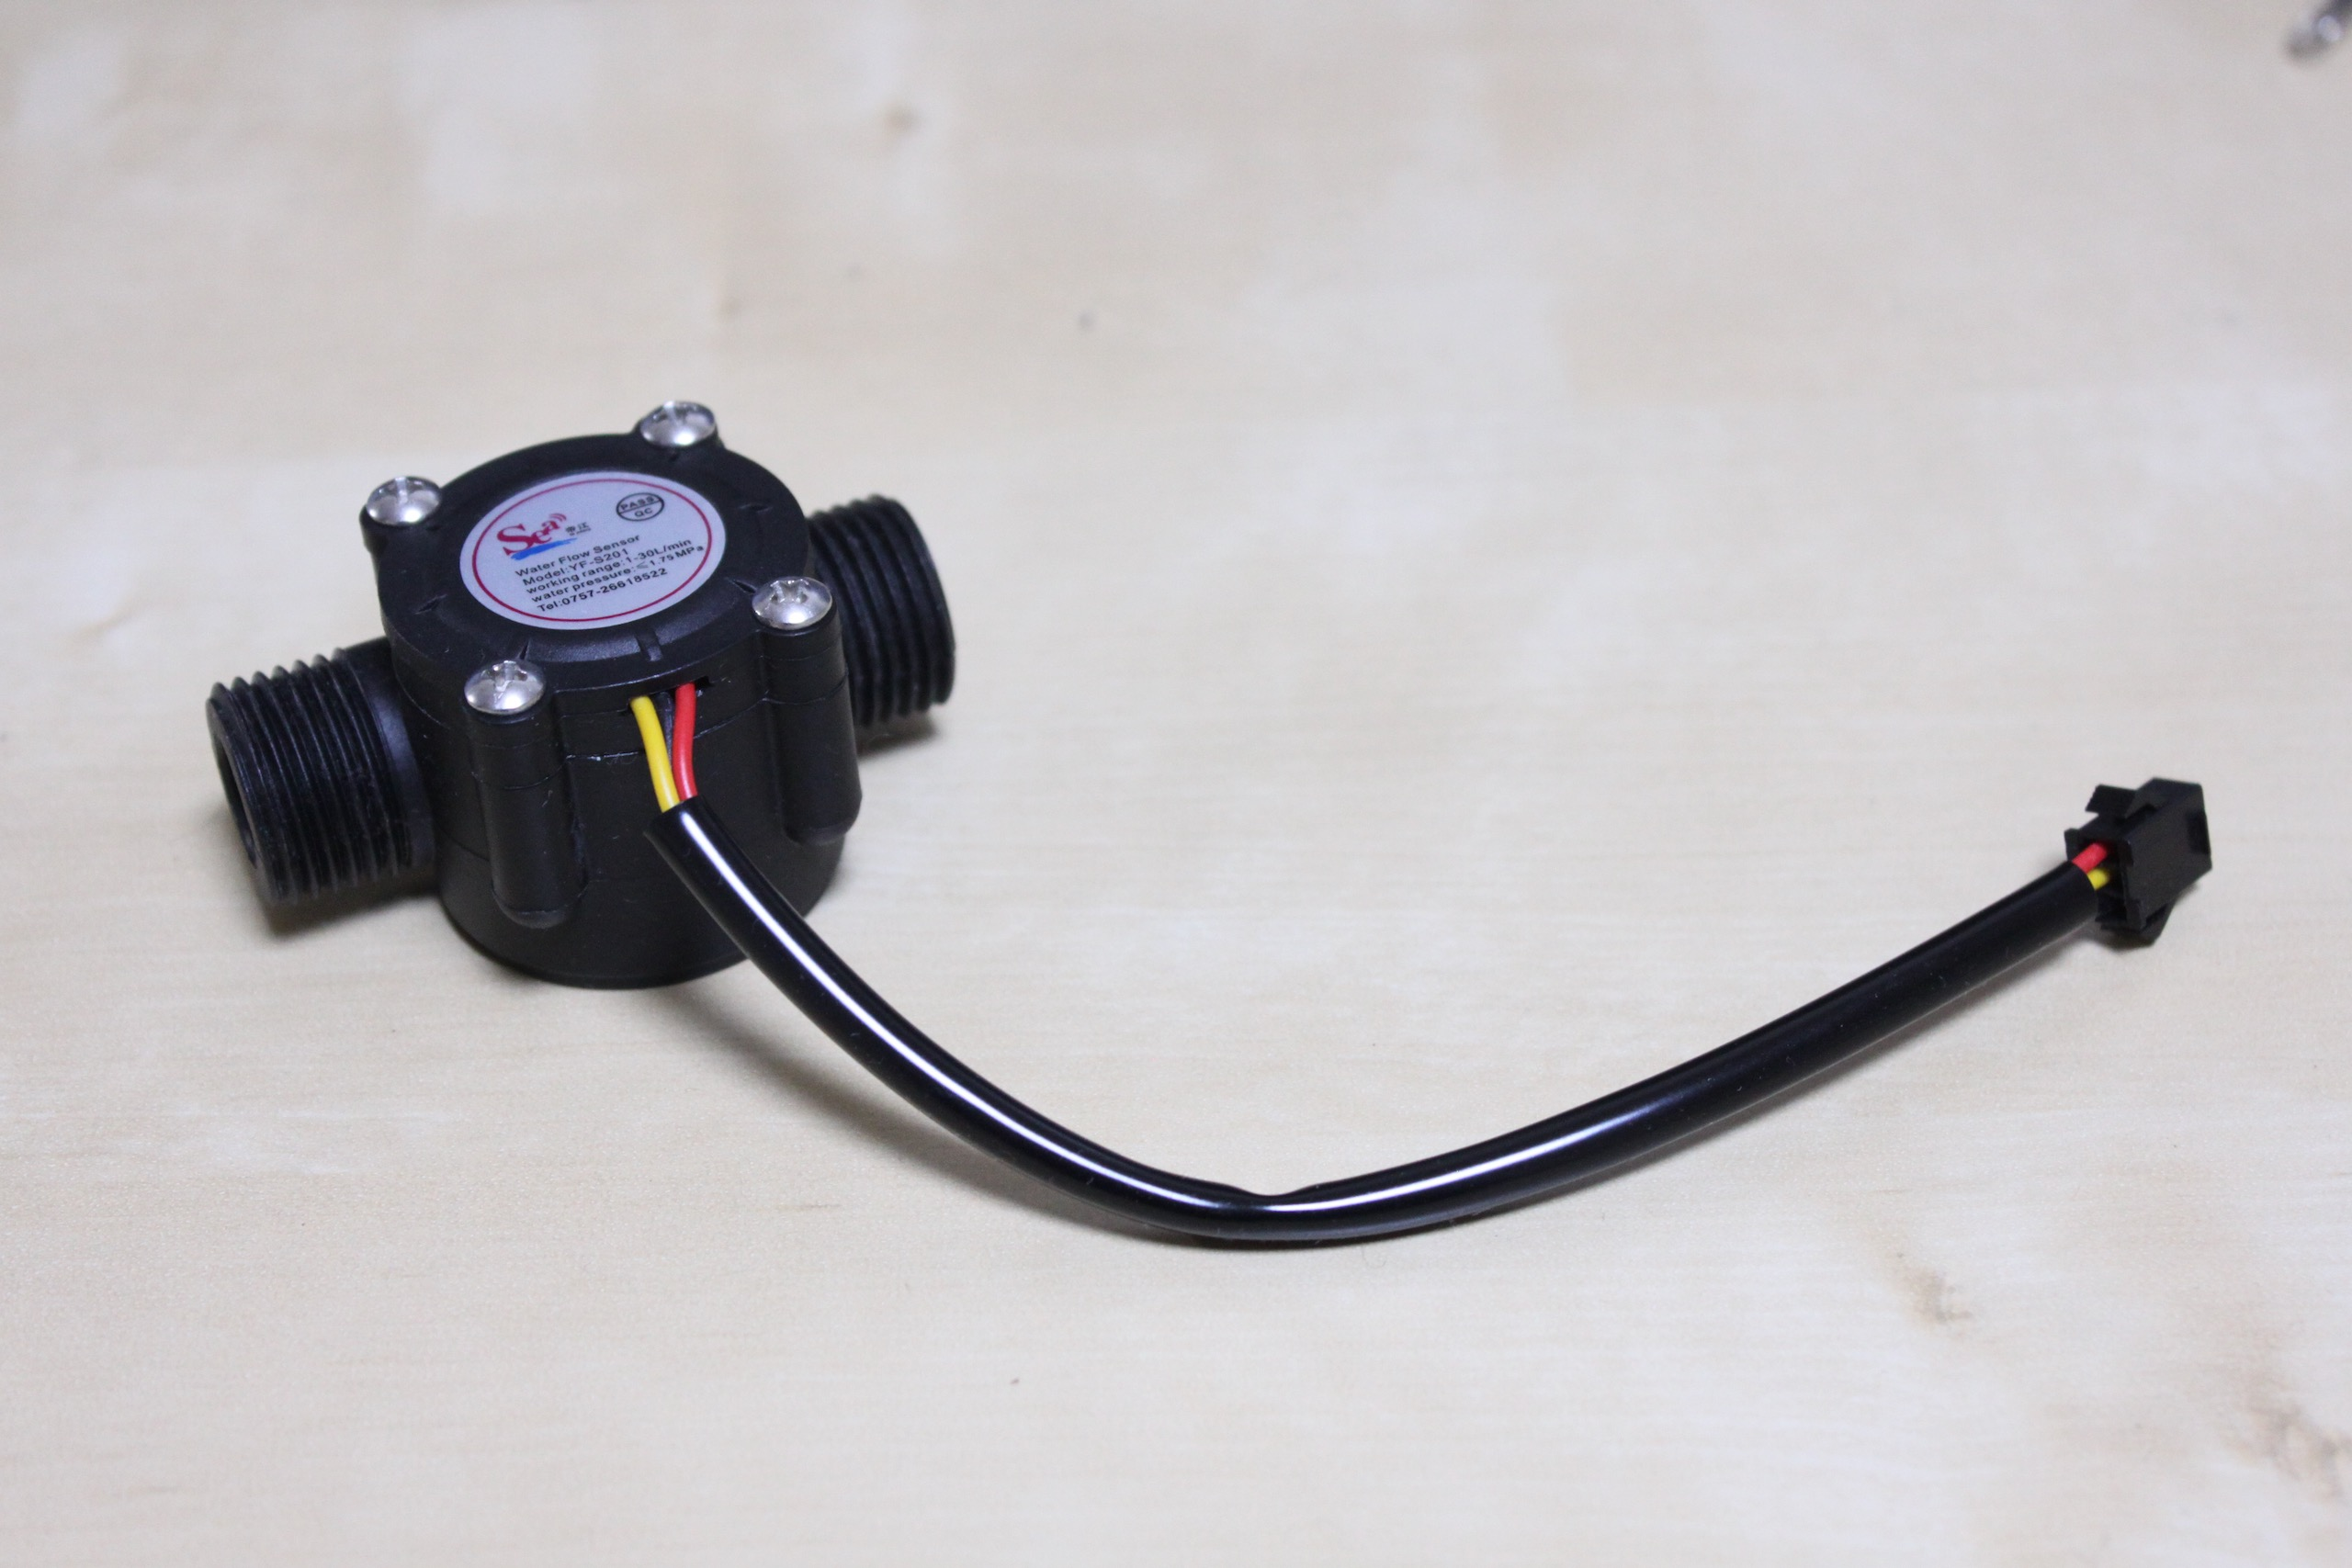
\includegraphics[width=8cm]{fig/yf-s201}
    \caption{水流計 YF-S201}
    \label{fig:yf-s201}
  \end{center}
\end{figure}

\begin{table}[H]
\begin{center}
\begin{tabular}{|l|l|}
\hline
回転数測定方式 & ホール素子                    \\ \hline
本体素材    & PVC                      \\ \hline
インペラ素材  & POM                      \\ \hline
重量      & 49.5g(実測値)               \\ \hline
流路外径    & 20mm                     \\ \hline
流路入口内径  & 9mm                      \\ \hline
流路出口内径  & 12mm                     \\ \hline
動作流量    & 1-30L/min                \\ \hline
取付角度    & 90度\pm5度                 \\ \hline
流量-パルス  & 1L_{水}/min = 450_{pulse} \\ \hline
\end{tabular}
\caption{YF-S201 主な仕様}
\label{tb:YFS201_specsheet}
\end{center}
\end{table}

\ref{sec:correct_method}で述べたように,最大作業の測定を行う場合には呼気が流れる流路の内径は35mm以上必要であるという.今回使用したYF-S201は最小径が9mmとなっているため,必要とされる35mmの場合に比べて断面積比で7\%程度の流路断面積となっていることになる.このことから,今回製作した装置は最大作業の測定には使用できないことになる.今回は呼吸代謝測定装置を安価に製作することが目的であり,最大作業の測定を考慮しないこととした.

\subsubsection{タービン式流量計の空気流量係数の測定}
\label{sec:measuring_coefficient}

表\ref{tb:YFS201_specsheet}の仕様によれば,YF-S201は1分あたり水流1Lが流路を流れる時に1分あたり450個の矩形波を出力する.ただし,これは水流が流れる時の値なので,空気の流量計として使用するためには空気が流れる際の関係式を求める必要がある.また,使用する呼気収集マスク\ref{fig:mask_front}に水流計を取り付けた際に,取付角度は仕様の90度\pm5度を外れ,顔が正面を向いた状態で60度程度となる.そこで,今回は取付角度が60度の場合に流体として空気が流れる場合の流量-パルス値を実験で求めた.

今回は流量計を図\ref{fig:mask_front}のように逆流防止弁の先に取り付ける.また,呼気の流量は一呼吸の内,吸気が終了した時点の0から最も強く息を吐き出す最大の範囲で常に変動する.これにより,呼気の流量は,吸気中は逆流防止弁が閉じているため0になり,呼気開始とともに逆流防止弁が開き次第に大きくなり,呼気終了時点で瞬時に0になる.そこで,一定流量の空気を流し続けた際の値を求めるのではなく,YF-S201が{\bf 一定量の空気が流れた際のパルス数が毎回等しくなるということを仮定}し,パルス数あたりの流れた空気の容量を求めるための係数を求めることで,水流計を使って空気の流量を測定する.

\begin{figure}[H]
  \begin{center}
    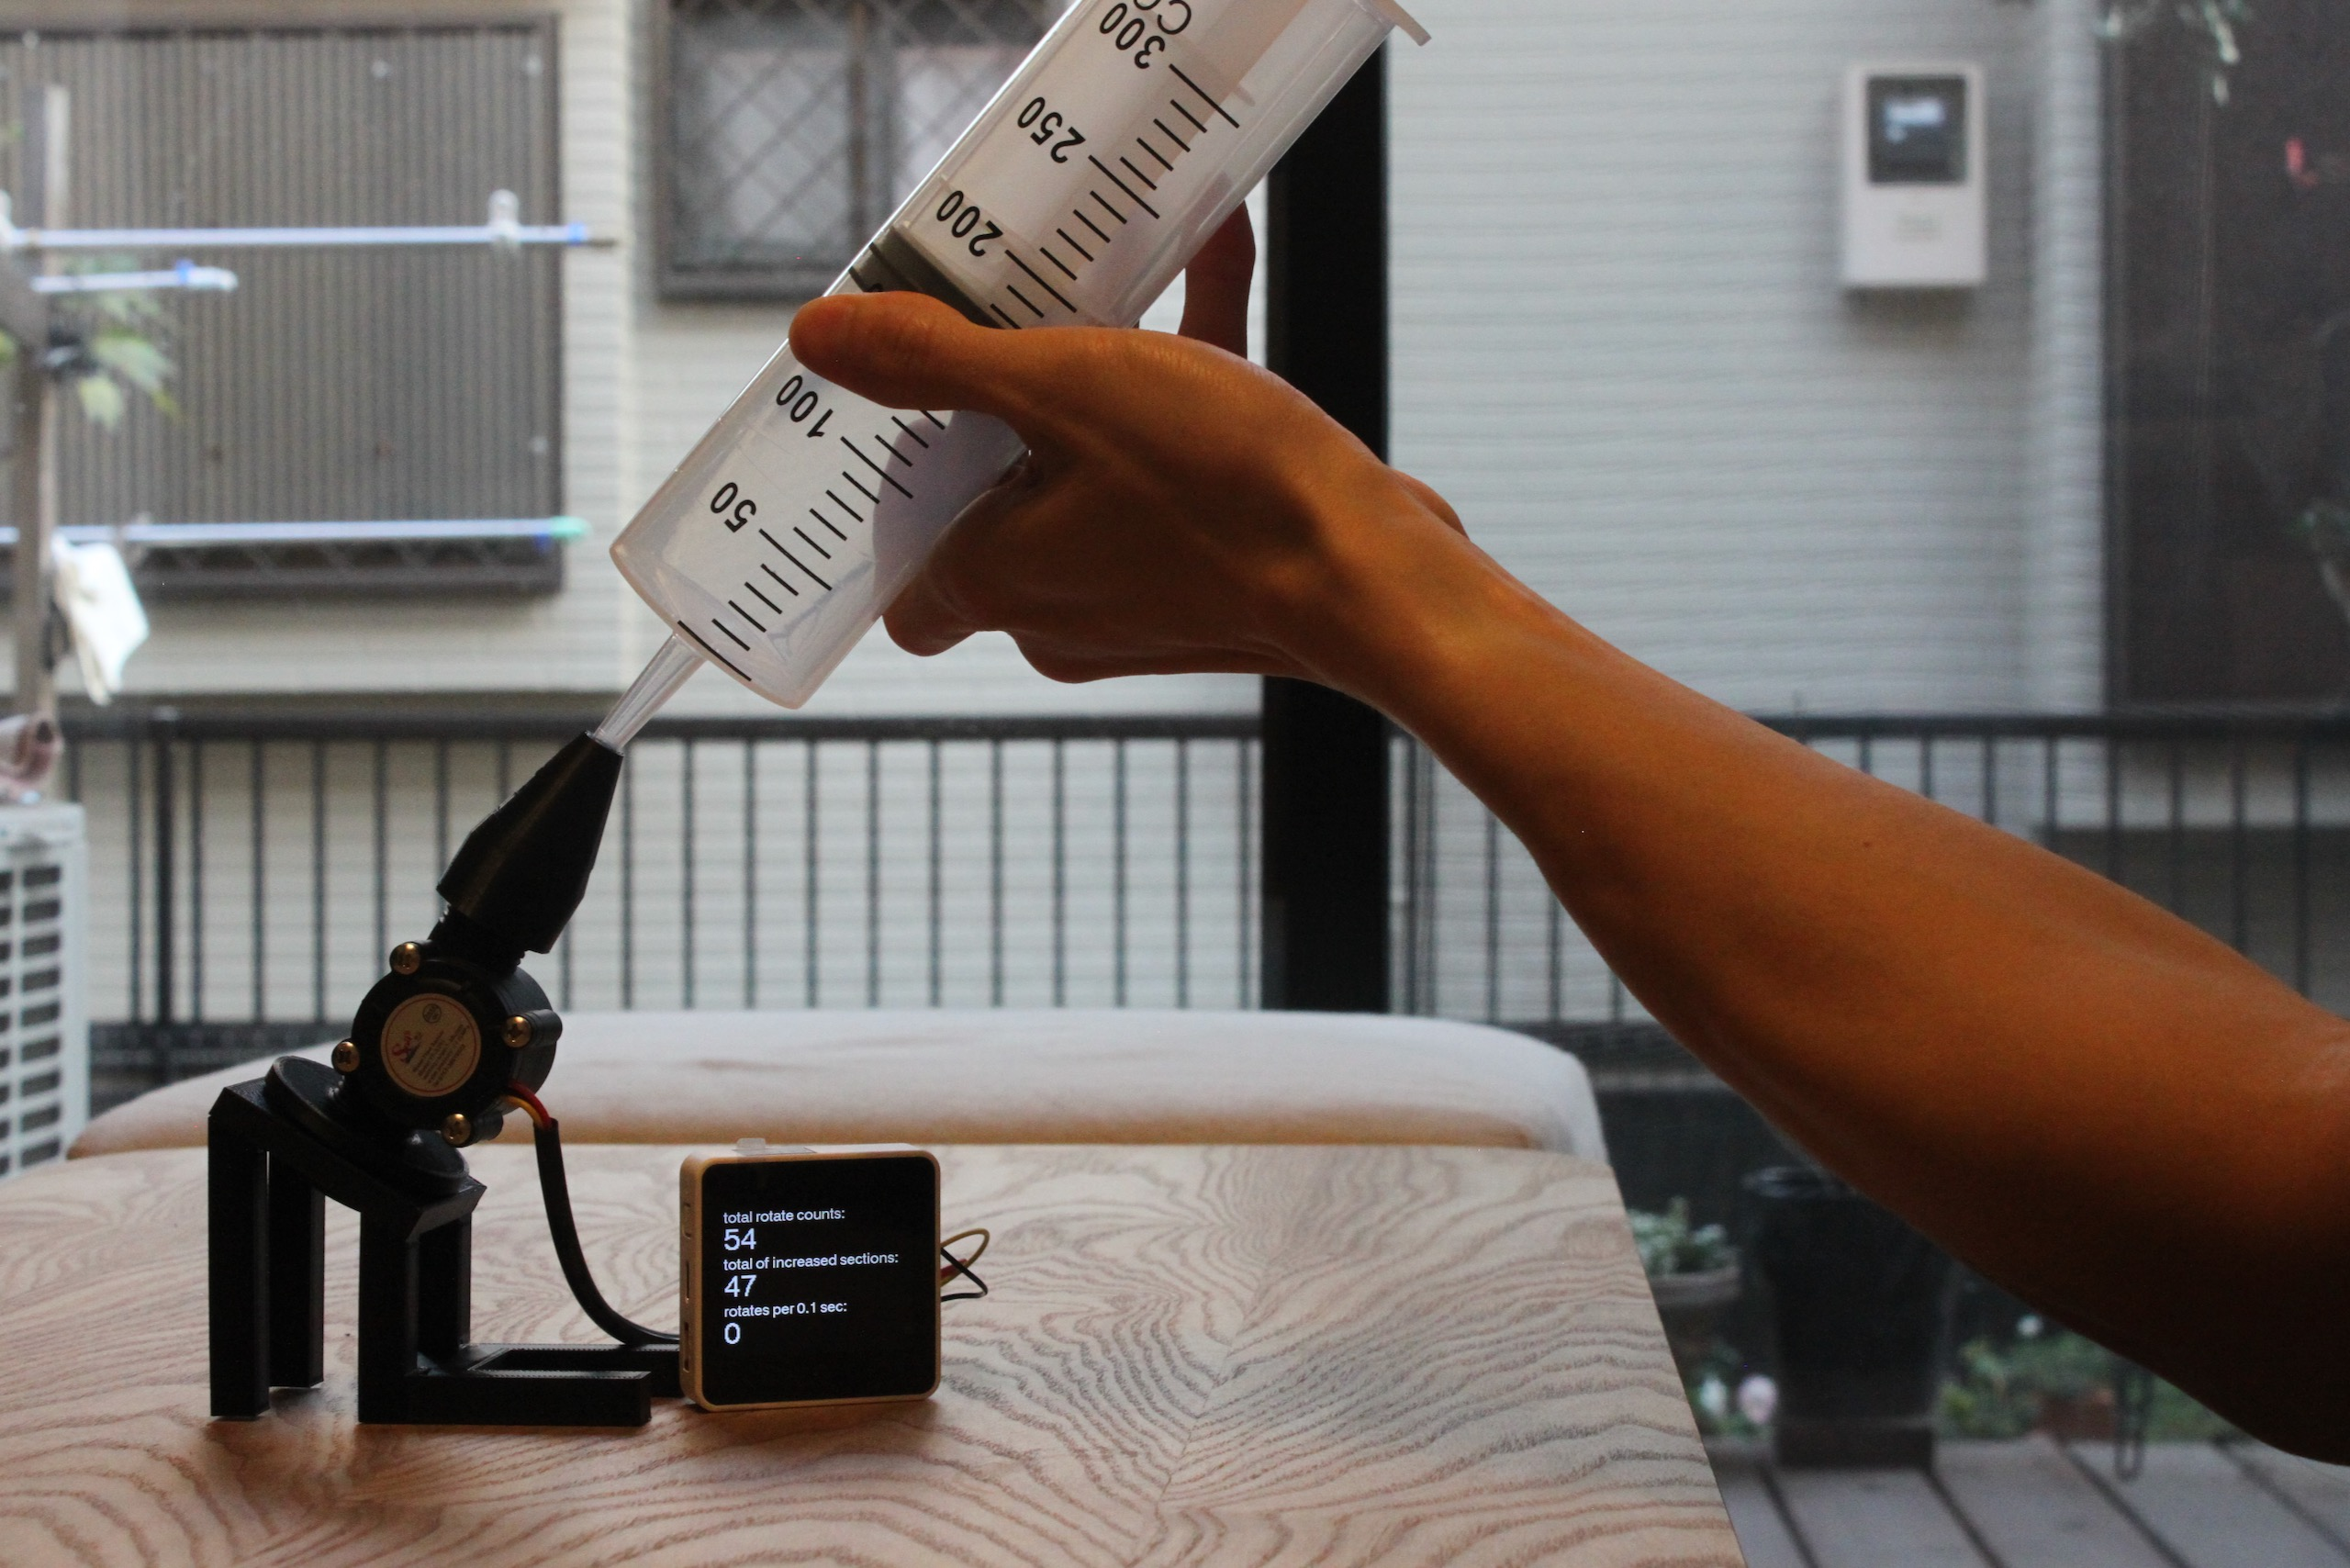
\includegraphics[width=10cm]{fig/flowsensor_calibrate}
    \caption{流量係数測定の実験}
    \label{fig:flowsensor_calibrate}
  \end{center}
\end{figure}

図\ref{fig:flowsensor_calibrate}は実験の様子である.空気の量を正確に測りとれるシリンジを水流計の入り口に接続し,一定量の空気を送り込んだ時のパルスの数を測定した.送り込む空気の量は,入手が可能であったシリンジの最大サイズから300mLとした(図\ref{fig:syringe}).シリンジのピストンを押す速さが出来る限り一定になるように注意しながら手でピストンを押した.シリンジと流量計の接続部は空気が漏れないようにするために,シリンジのノズル先端と流量計の入り口を接続する逆漏斗状のジョイント部品を3Dプリンターで製作した.ジョイント部品には,シリンジのノズルから出た高圧の空気が流量計のタービンに直撃するのを避けるため,図\ref{fig:syringe_cone}のように,ノズルから出た空気が一度中央の壁に当たって跳ね返り,周囲から水流計へと流れる形状となっている.また,実際に取り付ける状態を想定して流量計の角度を60度に保つために,3Dプリンターで台座を製作した.

\begin{figure}[H]
  \begin{center}
    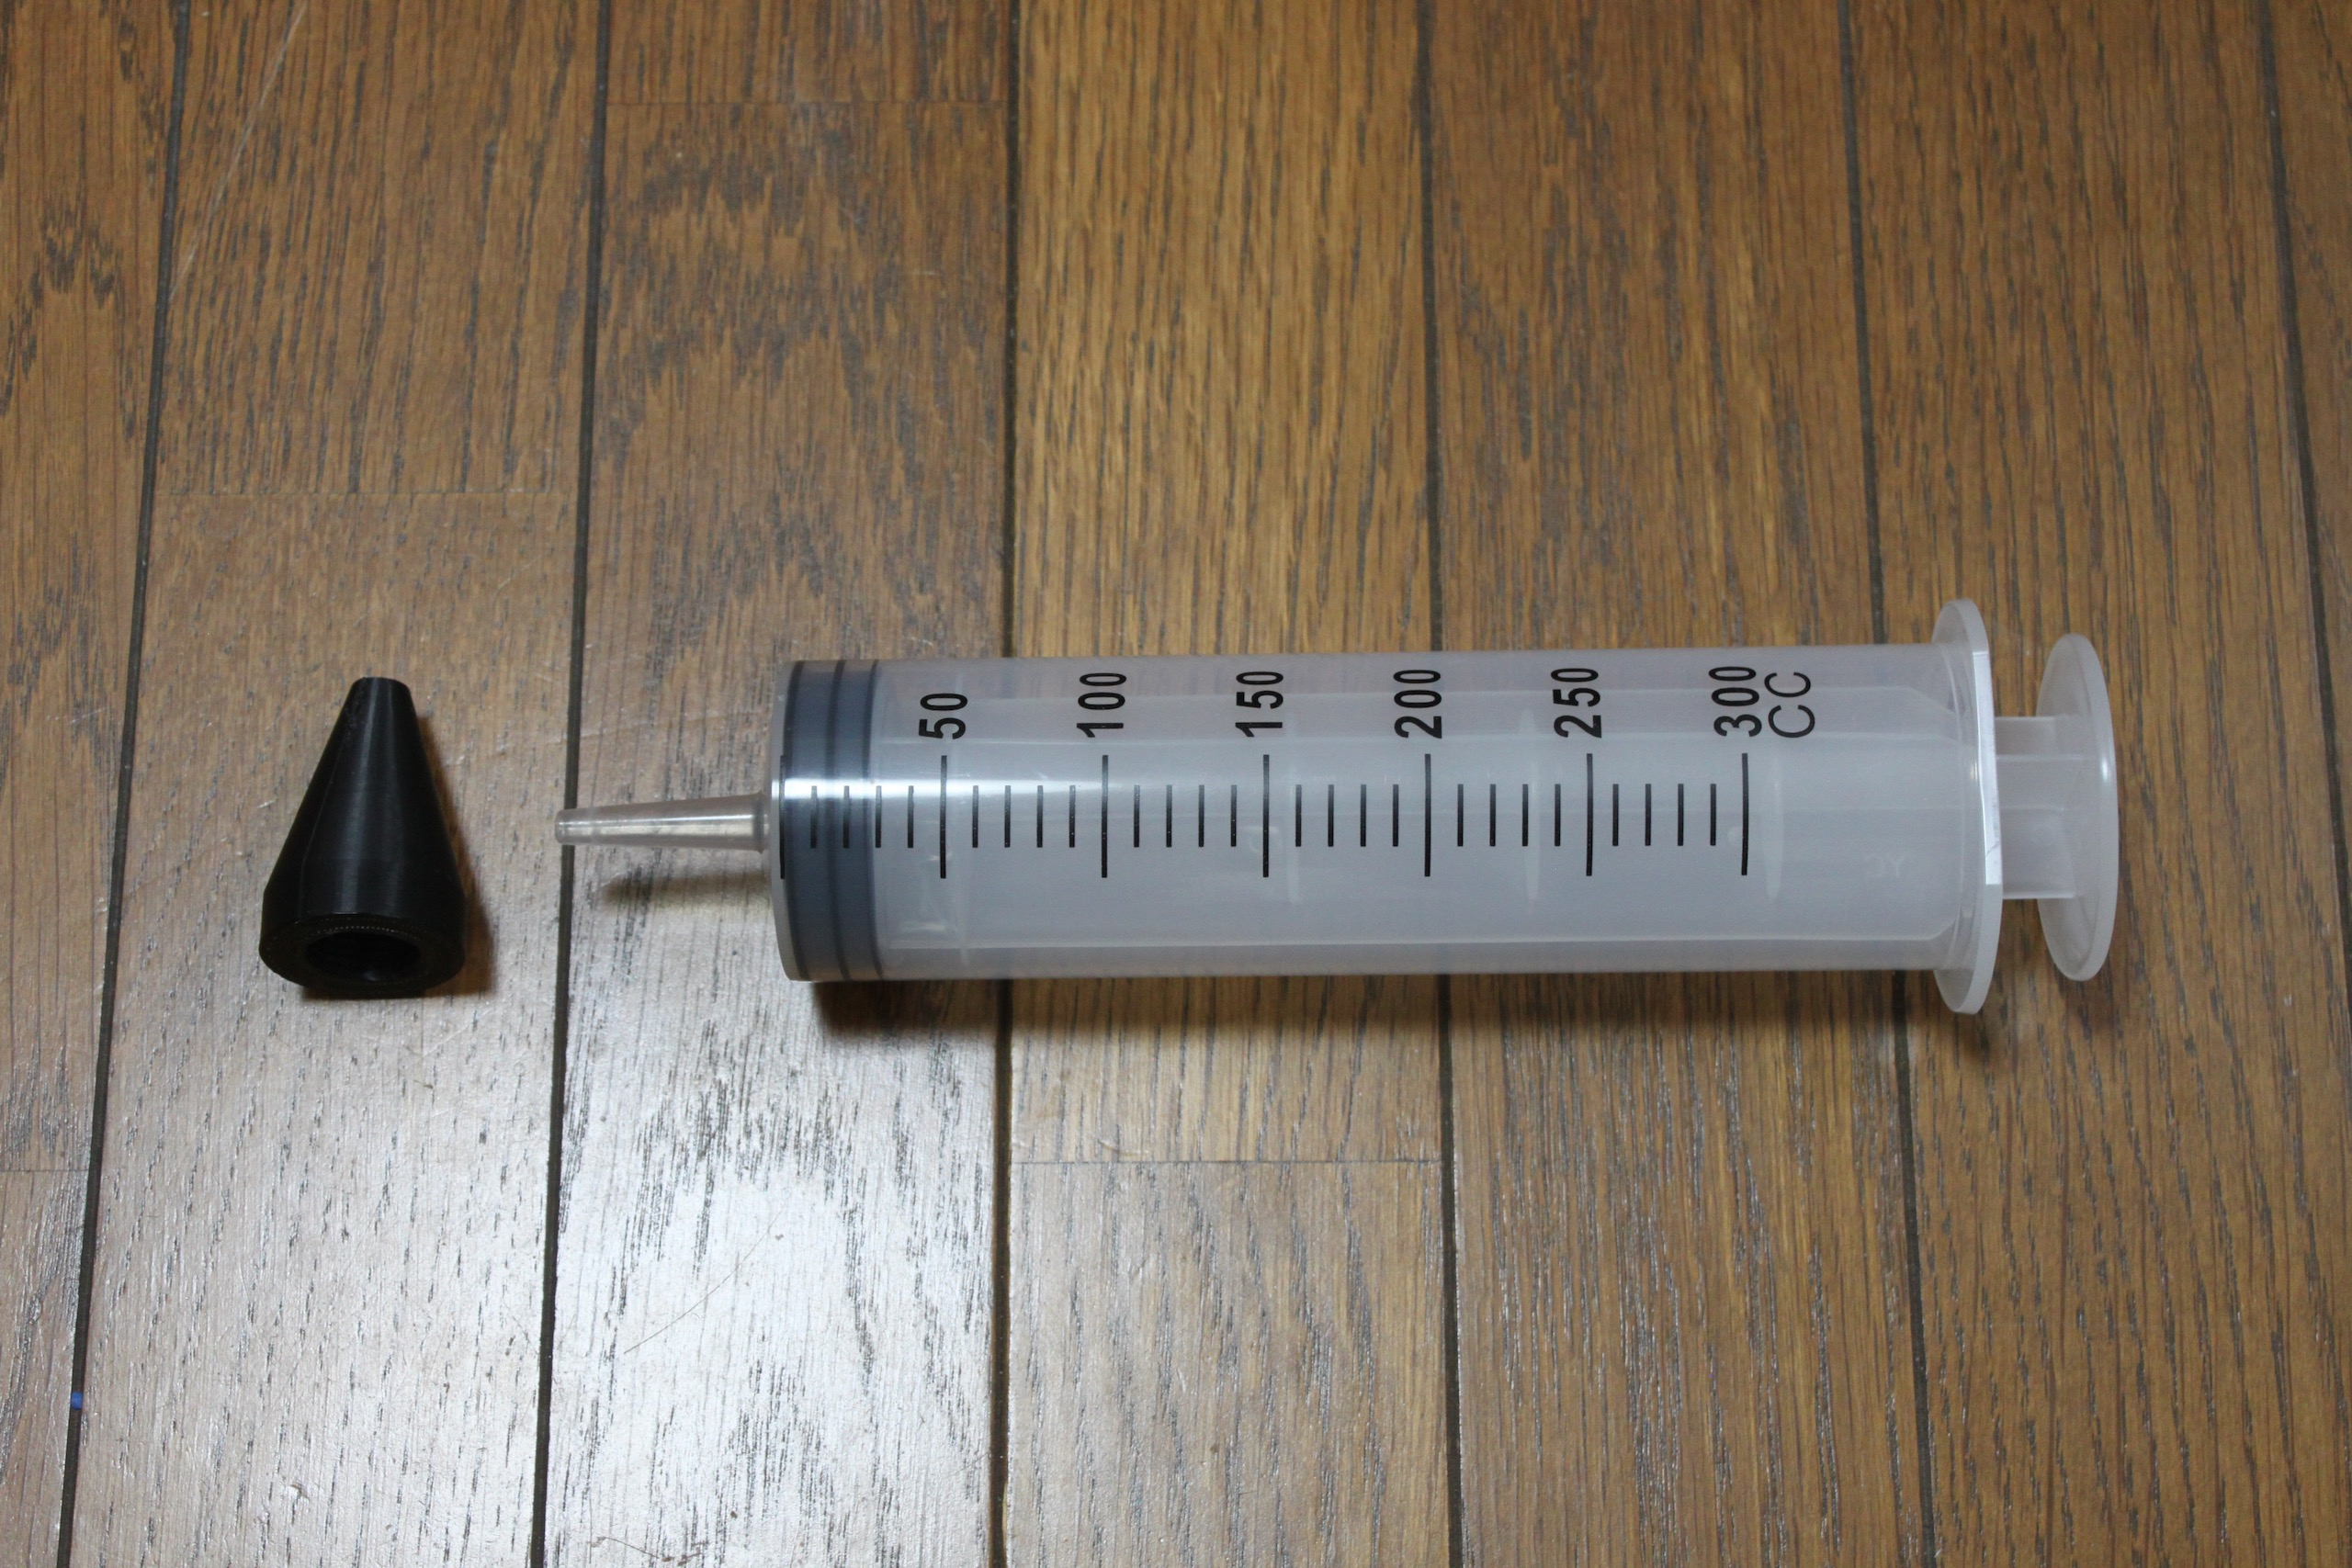
\includegraphics[width=8cm]{fig/syringe}
    \caption{接続用ジョイント部品とシリンジ}
    \label{fig:syringe}
  \end{center}
\end{figure}

\begin{figure}[H]
  \begin{center}
    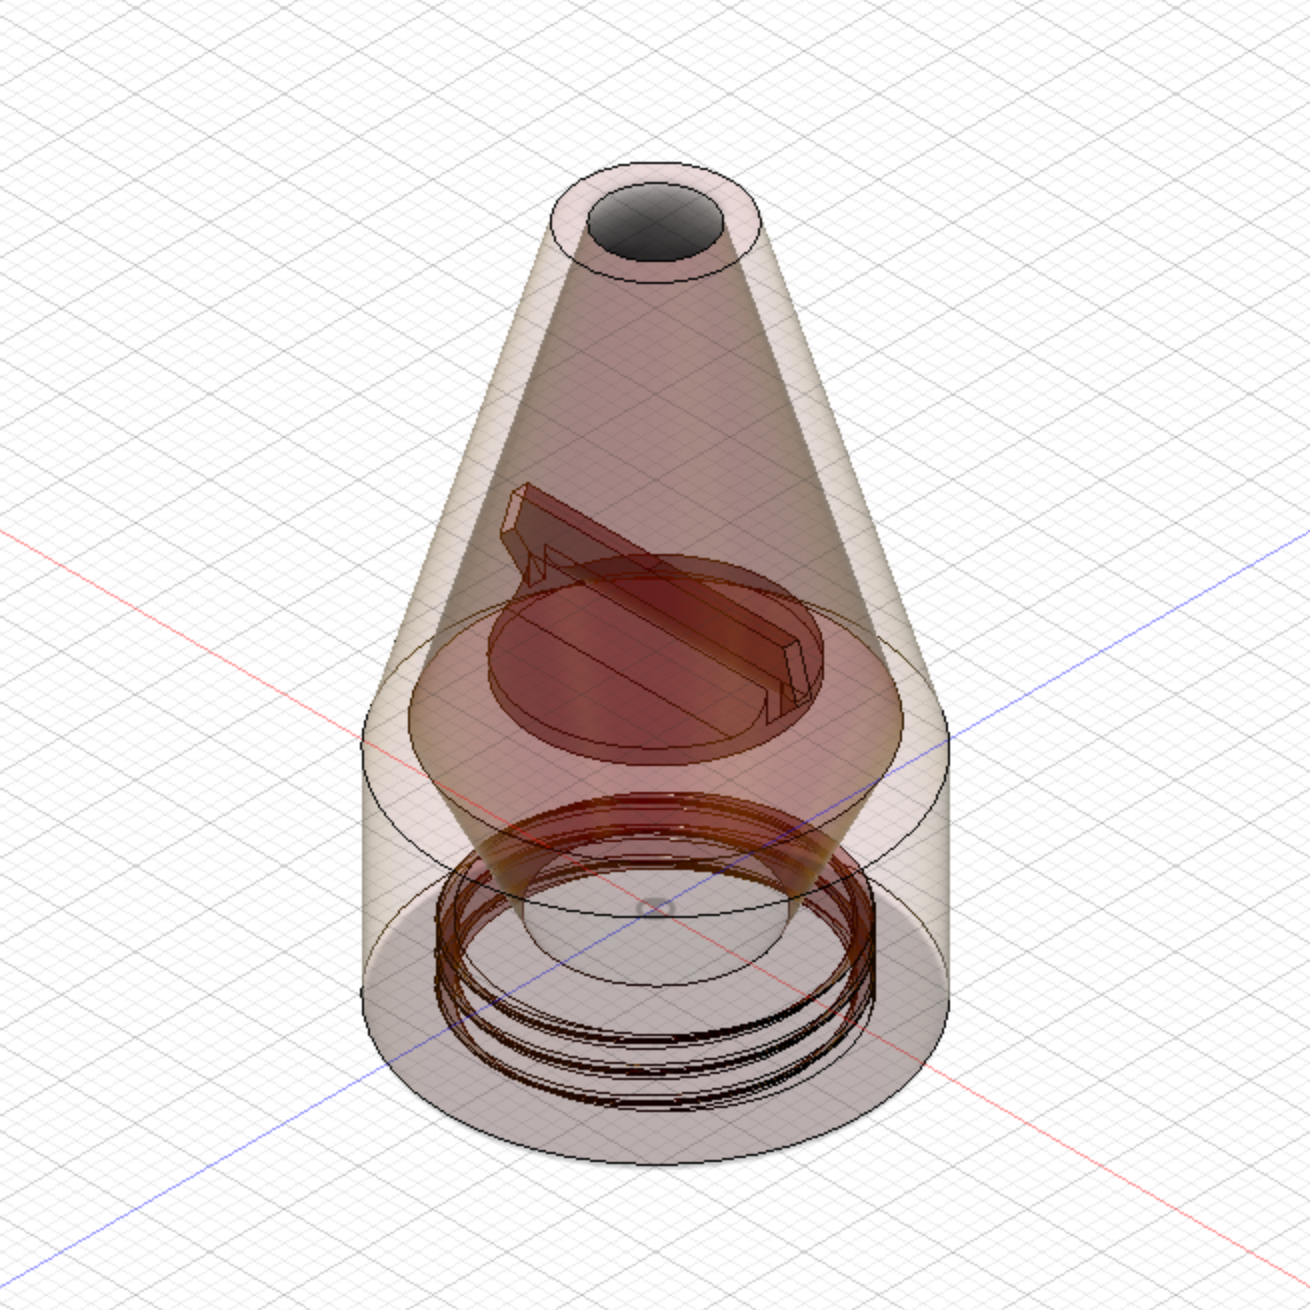
\includegraphics[width=8cm]{fig/syringe_cone}
    \caption{ジョイント部品の構造}
    \label{fig:syringe_cone}
  \end{center}
\end{figure}

今回の装置では流量計を呼気側の逆流防止弁の排気側に取り付ける.実際の呼気流量は呼気が終了し逆流防止弁が閉じた時点で0になるが,実際には流量計のタービンが空転することにより,実際には呼気が行われていない分の呼気流量を測定することとなってしまう(図\ref{fig:flowsensor_increased_section}).そこで正しく呼気流量を測定するためにはこの空転分の区間を除外する必要がある.一呼吸の内で呼気が行われ逆流防止弁が開いている間,呼気の流量は増加し続ける.このことから,流量計のタービンの時間あたりのパルス数を0.1秒ごとに算出し,これが増加から減少に転じた時間までのパルス数を係数の算出に用いた.以上の処理を行い,空転分を除外した回転数を計測するプログラムを作成しM5Stack Core2で動作させてパルス数を測定した.

\begin{figure}[H]
  \begin{center}
    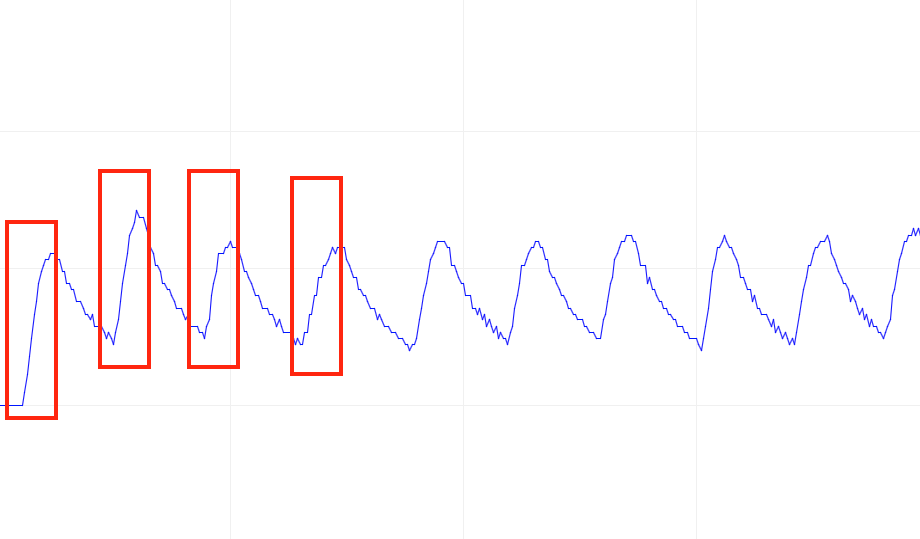
\includegraphics[width=8cm]{fig/flowsensor_increased_section}
    \caption{青線:流量計が出力する流量(パルス数),赤枠線:実際の流量(パルス数)}
    \label{fig:flowsensor_increased_section}
  \end{center}
\end{figure}

測定は200回行い.200回の測定で求められたパルス数の代表値を空気300mLあたりのパルス数とする.結果は以下の通りであった.

\begin{table}[H]
\begin{center}
\begin{tabular}{|l|l|}
\hline
平均値  & 49.59      \\ \hline
中央値  & 50         \\ \hline
最頻値  & 50         \\ \hline
最大値  & 71         \\ \hline
最小値  & 27         \\ \hline
標準偏差 & 8.22203746 \\ \hline
\end{tabular}
\caption{300mLの空気を流した際,YF-S201が増加区間で出力するパルス数}
\label{tb:flowsensor_result}
\end{center}
\end{table}

\begin{figure}[H]
  \begin{center}
    \caption{結果のヒストグラム}
    \label{fig:flowsensor_histogram}
    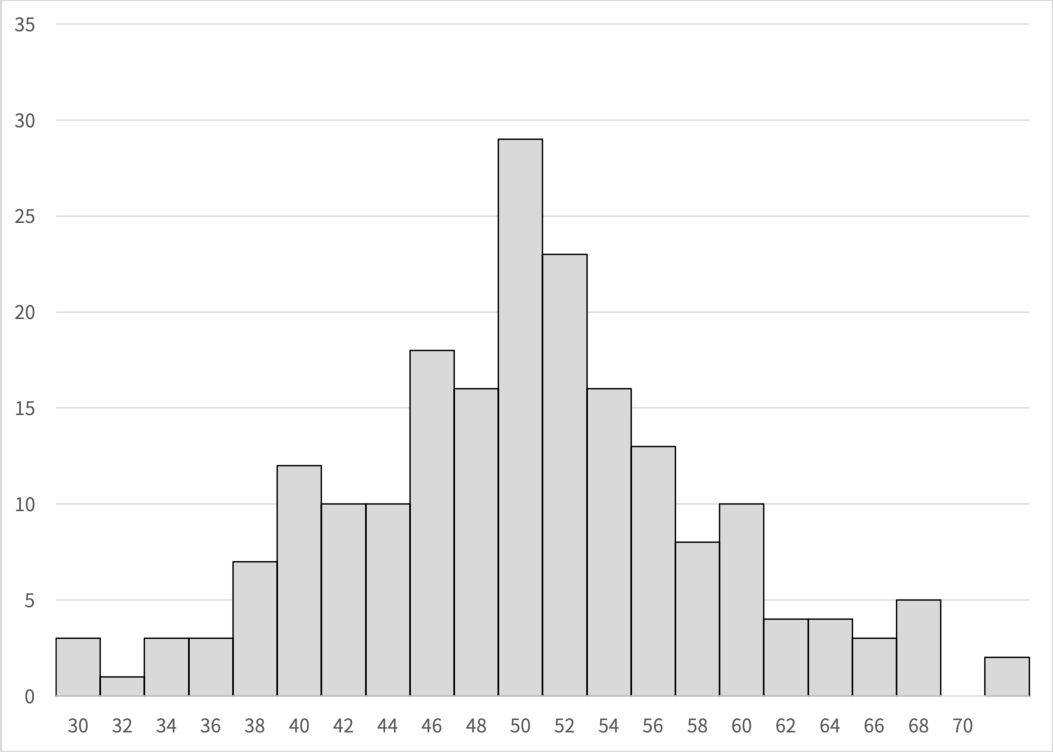
\includegraphics[width=10cm]{fig/flowsensor_histogram}
  \end{center}
\end{figure}

表\ref{tb:flowsensor_result}とヒストグラム\ref{fig:flowsensor_histogram}から,パルス数は正規分布をとることが分かる.よって,今回は平均値の整数値,かつ中央値,最頻値となる50を採用する.

流量計YF-S201に300mLの空気が流れた際のパルス数が50であることより,YF-S201がパルスを一つ出力する(タービンが一回転する)時,流れた空気の量{\it x}(mL)は以下のようになる.

\begin{equation}
  \label{eq:pulse_per_ml}
  x = \frac{50}{300} = \frac{1}{6} = 0.1666666667 (mL)
\end{equation}

これにより,単位時間ごとのパルス数にこの係数を掛けることで流量を求めることができる.

\subsection{呼気酸素濃度の測定}

酸素濃度の測定には,酸素と化学的に反応して起電力を発生する物質を用いて,発生する電圧を測定することによって濃度を測定する方法が使われる.主なものにはジルコニア式とガルバニ電池式があり,ジルコニア式は動作のためには高温を維持する必要があるため,呼気分析にはガルバニ電池式が用いられる.

\subsubsection{空気亜鉛電池酸素濃度計}
\label{sec:o2sensor_a-5s}

今回は株式会社ピーバンドットコムから発売されている「実習用酸素センサキット A-5S」(以下「A-5S」)は,補聴器などに用いられる安価な空気亜鉛電池を利用した酸素センサーである.空気亜鉛電池が空気中の酸素と反応することで発生する電圧を測定することで酸素濃度を測定することができる.東京工業高等専門学校の髙橋三男教授によって開発され,株式会社ピーバンドットコムによって量産されている.秋月電子通商にて1個税込み1100円で販売されている.

\begin{figure}[H]
  \begin{center}
    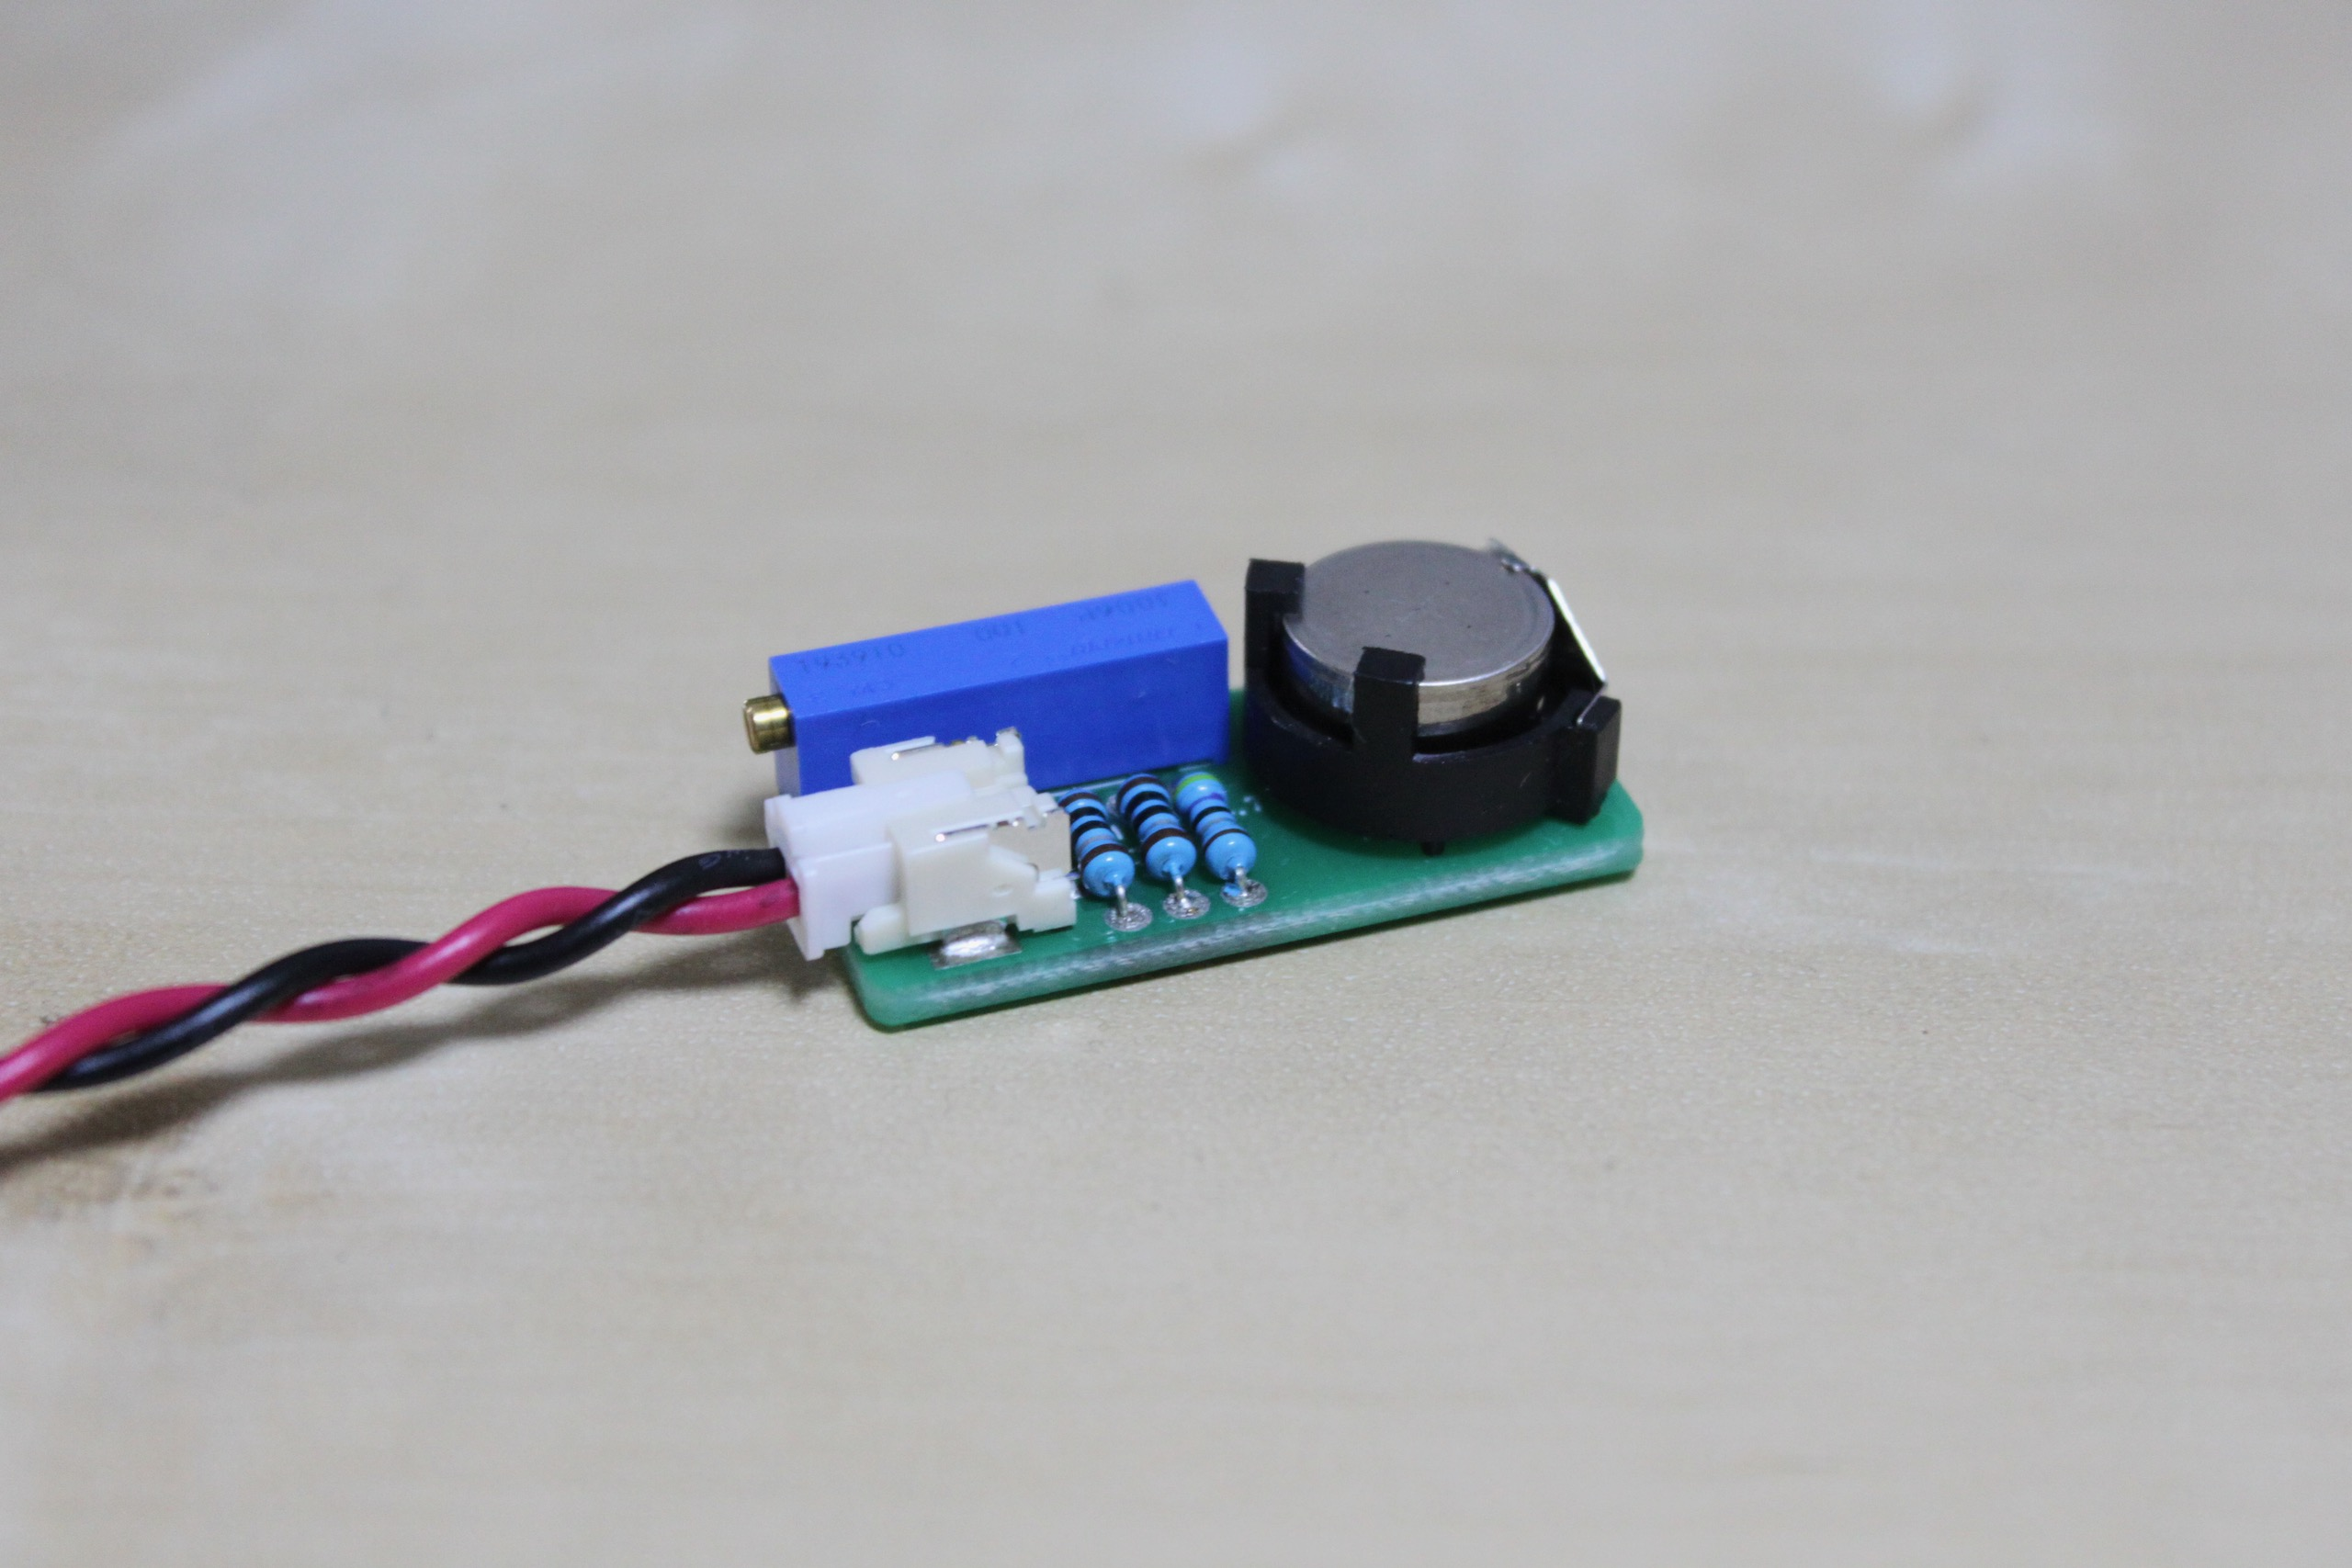
\includegraphics[width=8cm]{fig/a-5s}
    \caption{実習用酸素センサキット A-5S}
    \label{fig:a-5s}
  \end{center}
\end{figure}

空気亜鉛電池は負極に亜鉛,正極に酸素を使用し,起電力を発生する燃料電池の一種である.空気亜鉛電池自体も6個入りで500円程度と安価に入手が可能だが,その原理から,極度な乾燥・多湿,2000ppmを大きく上回るような高濃度の二酸化炭素濃度環境下における使用には向かないとされる.今回の装置では呼気を収集するミキシングチャンバー内で使用するため,常時湿度100\%の飽和水蒸気に晒され,最大90000ppm程度の二酸化炭素濃度において使用することになる.

A-5Sは,空気亜鉛電池に固定抵抗と可変抵抗を接続した構造になっている.可変抵抗を調整し,大気中の酸素濃度20.93\%に合わせてA-5Sから出力される電圧が20.93mVとなるようにキャリブレーションを行う.一般的なガルバニ電池式酸素濃度計が2年ほどの寿命を持つのに対して,A-5Sにおける空気亜鉛電池の寿命はおよそ25時間とされている.実際に検証を行ったところ,キャリブレーションをやり直すことで2日間ほどは同じ酸素亜鉛電池を使用して酸素濃度が可能であることを確認した.

今回はこのセンサーを,図\ref{fig:sensor_board}の通り二酸化炭素センサーとともに3Dプリンターで製作したミキシングチャンバーの円筒形状に合わせた台座上に設置した.なお,ミキシングチャンバー内での温度変化による抵抗値の変化を抑えるため,キットでは炭素抵抗が使用されている固定抵抗を金属皮膜抵抗に交換した上で使用している.

\begin{figure}[H]
  \begin{center}
    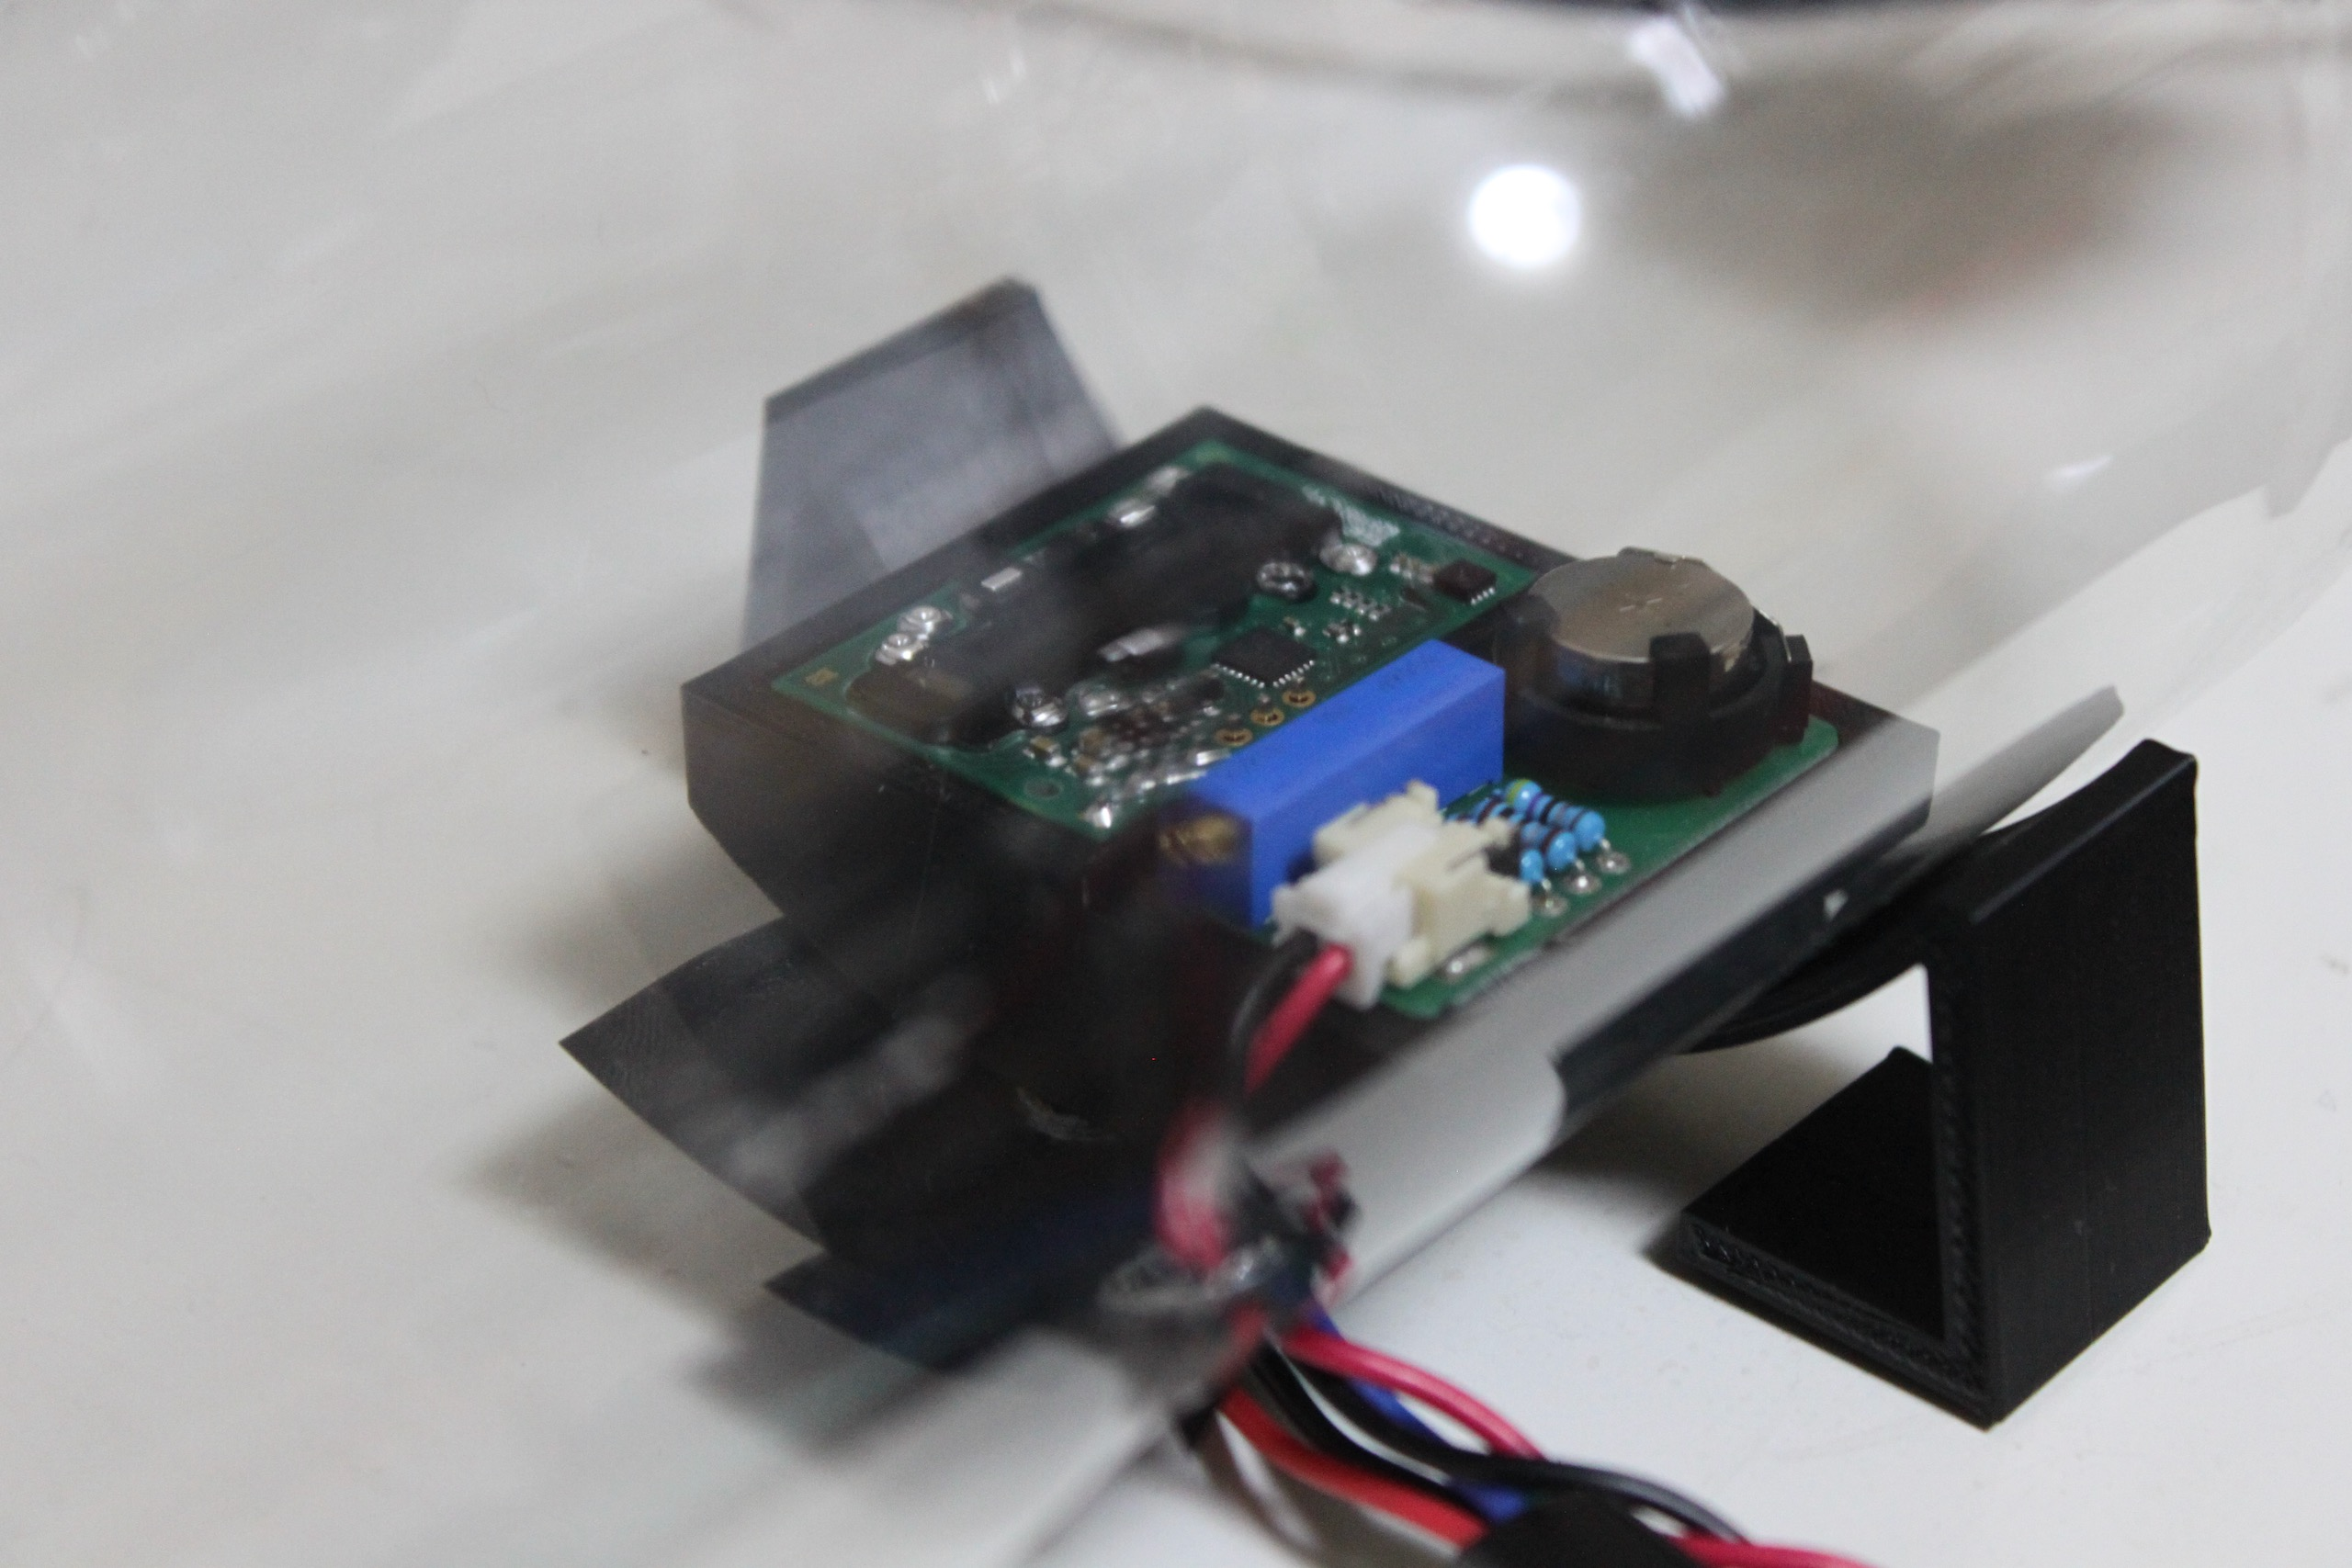
\includegraphics[width=8cm]{fig/sensor_board}
    \caption{ミキシングチャンバー内に設置したセンサー台座}
    \label{fig:sensor_board}
  \end{center}
\end{figure}

\subsubsection{電圧増幅}
\label{sec:opamp}

A-5Sが出力する電圧は正しくキャリブレーションされた場合において,酸素濃度20.93\%時に20.93mVと非常に微弱である.これをM5Stack Core2(ESP32)の12bit ADコンバーター(入力された電圧を0-4095の4096段階の数値に変換する)の測定範囲である0-3.3Vに合わせて電圧増幅を行った.

\begin{figure}[H]
  \begin{center}
    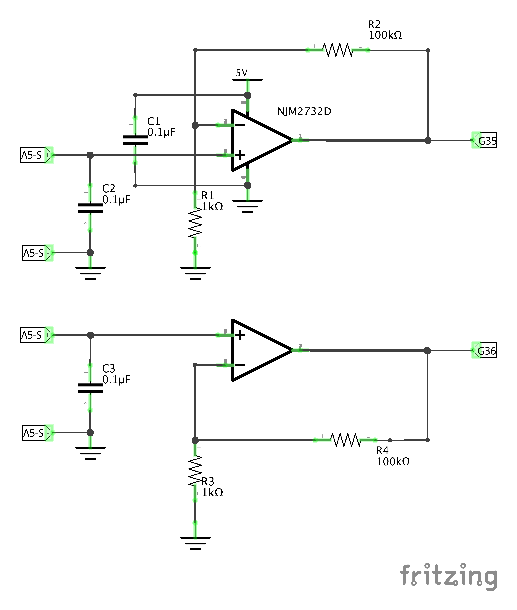
\includegraphics[width=12cm]{fig/a-5s_opamp_schematic}
    \caption{NJM2732Dによる非反転増幅回路}
    \label{fig:a-5s_opamp_schematic}
  \end{center}
\end{figure}

増幅にはオペアンプによる非反転増幅回路を用いた.単電源のフルスイングオペアンプであるNJM2732Dを使用して回路図\ref{fig:a-5s_opamp_schematic}の非反転増幅回路を製作した.増幅率は,ADコンバーターの測定範囲に合わせて,大気中の酸素濃度付近が測定範囲の中央に収まるように101倍とした.また,信号中のノイズを極力取り除くためにバイパスコンデンサーとしてセラミック積層コンデンサーを使用した.また,今回は呼気酸素濃度用の酸素センサーとしてA-5Sを一つだけ使用しているが,NJM2732Dは2回路入りのオペアンプであるため接地を兼ねてもう一回路分のターミナルも結線している.A-5Sをもう一つ追加し,吸気酸素濃度を測定することも可能である.

\begin{figure}[H]
  \begin{center}
    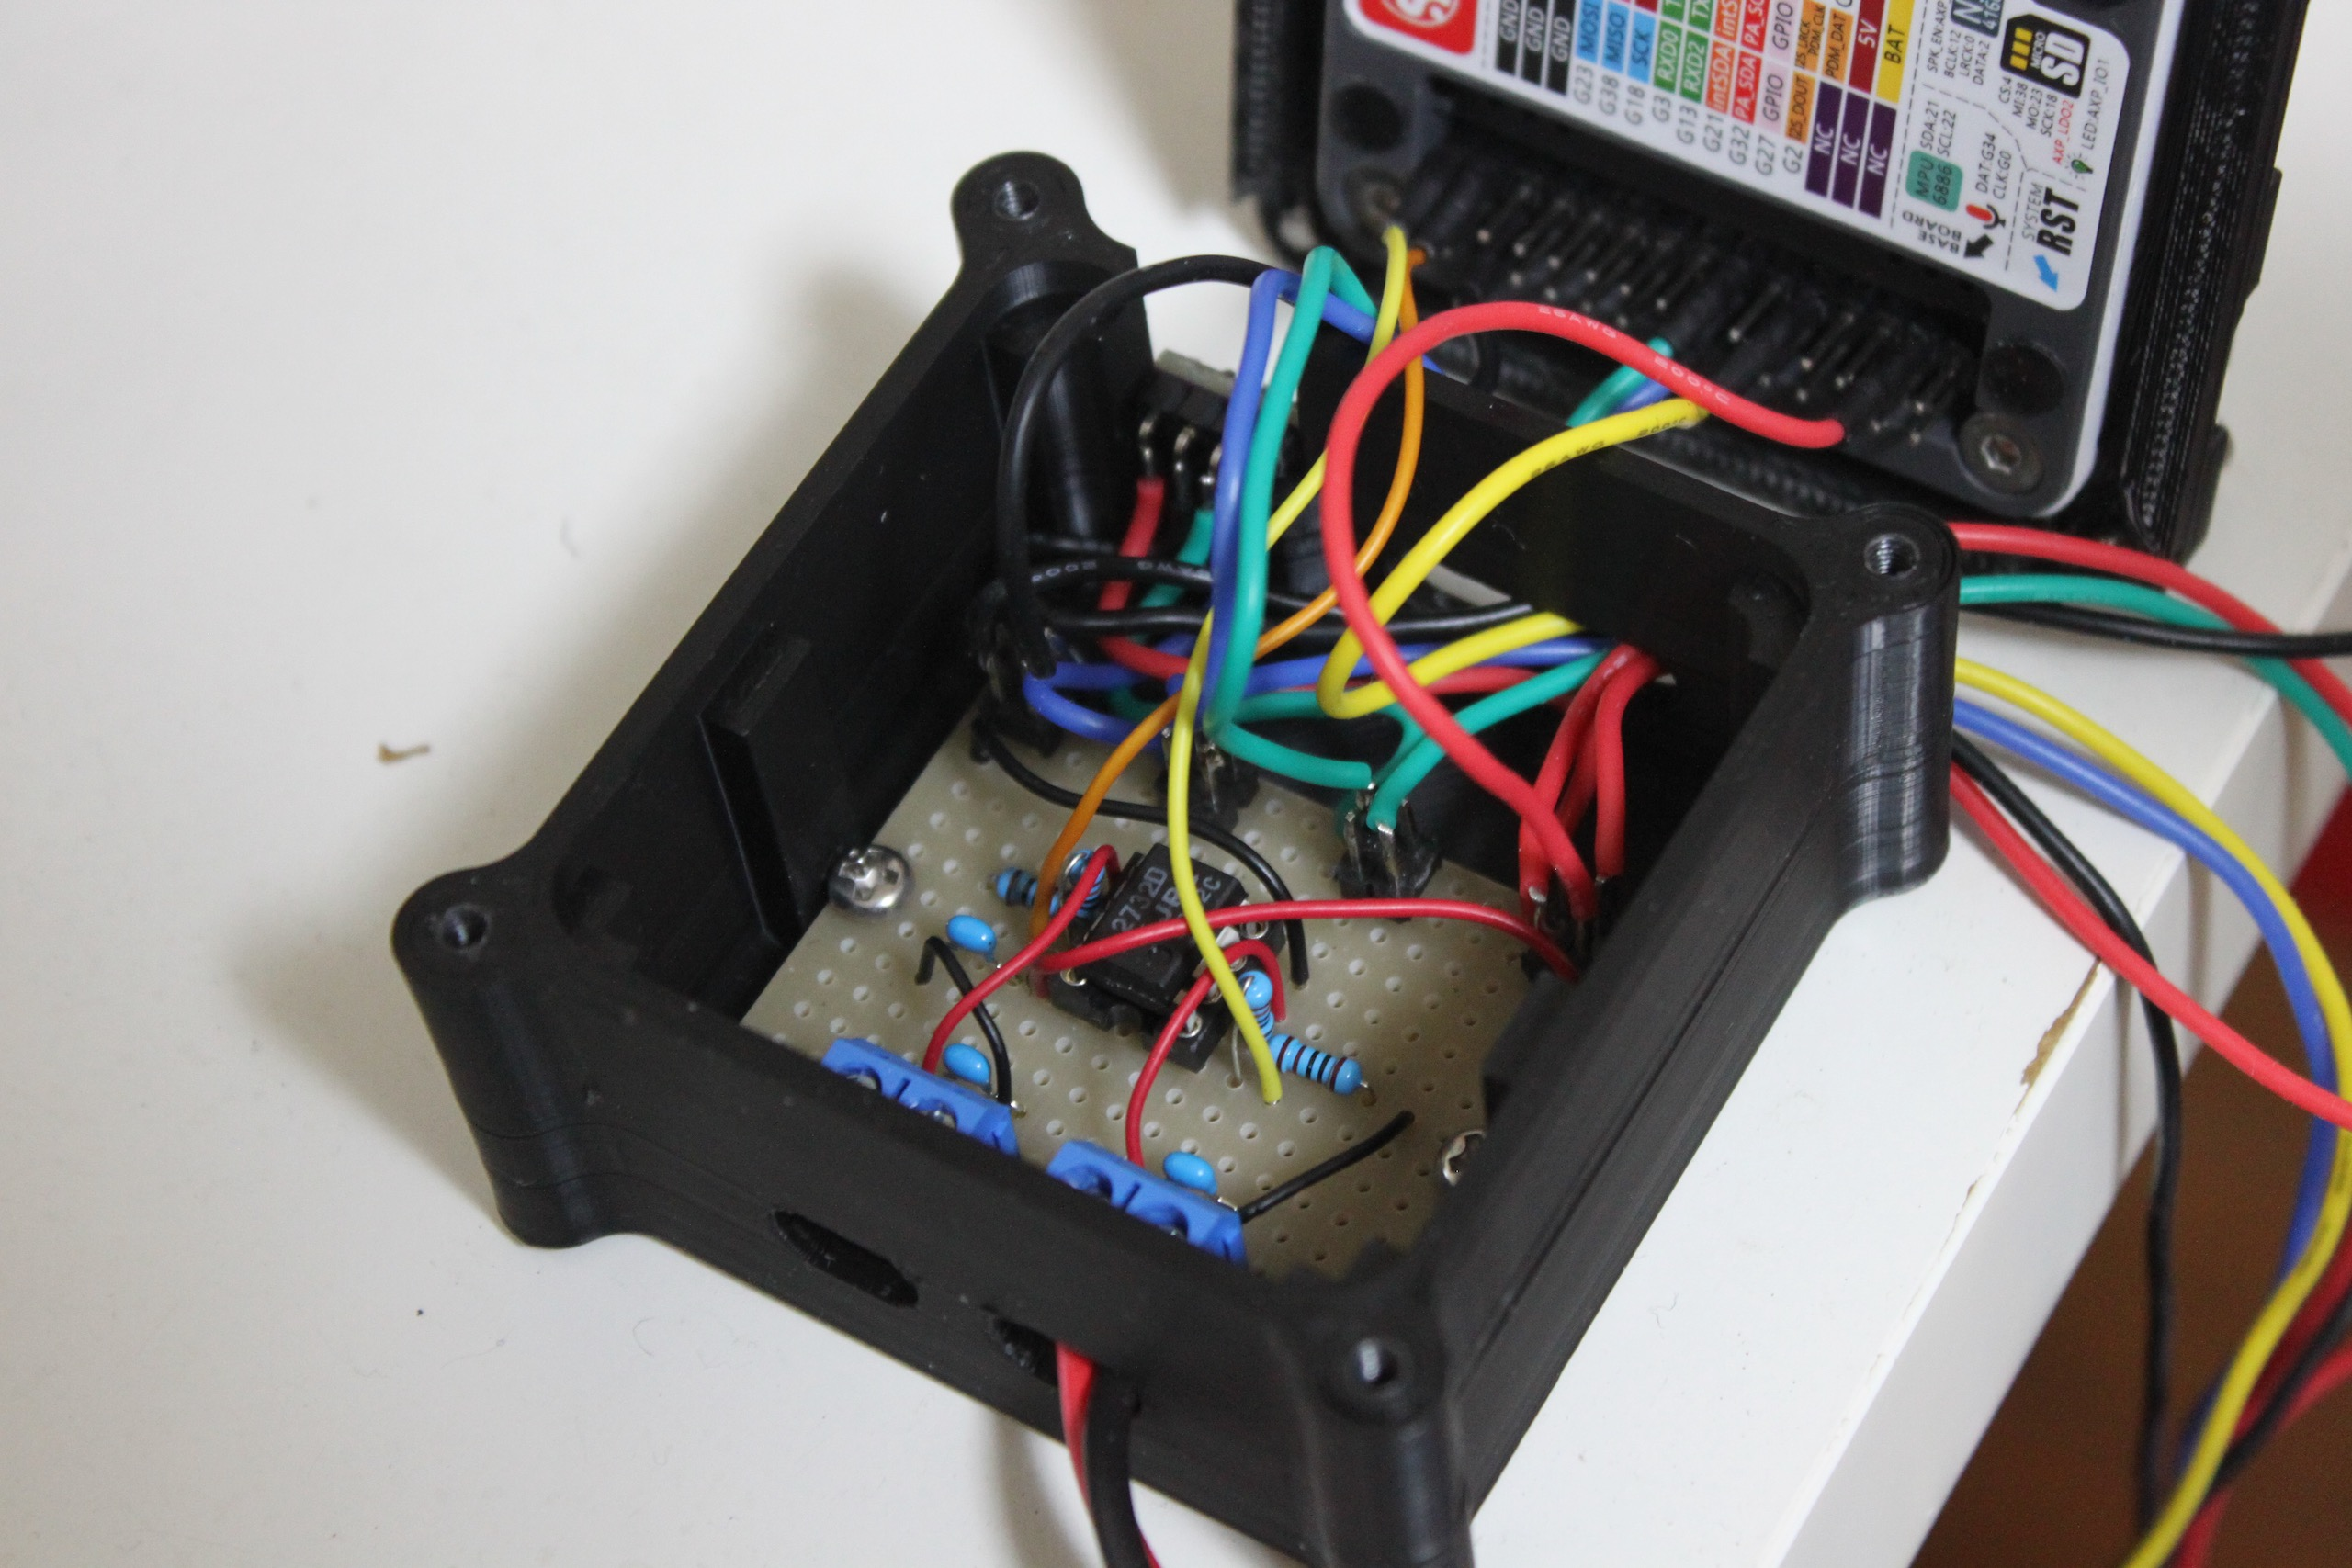
\includegraphics[width=8cm]{fig/opamp_universal}
    \caption{ユニバーサル基板上に実装した電圧増幅回路}
    \label{fig:opamp_universal}
  \end{center}
\end{figure}

この回路をユニバーサル基板に実装し,図\ref{fig:opamp_universal}のように筐体内のM5Stack Core2の下部に格納した.

\subsubsection{デジタルフィルターによるノイズ除去}

A-5Sが出力する電圧を図\ref{fig:a-5s_opamp_schematic}の回路で増幅した電圧をM5Stack Core2のADコンバーターで読み取ったところ,図のようにスパイク状に高い値が混ざるようなノイズが乗ることが分かった.これを取り除くためにプログラム上のデジタルフィルターで信号を平滑化した.今回使用したのは移動中央値フィルターである.

\begin{figure}[H]
  \begin{center}
    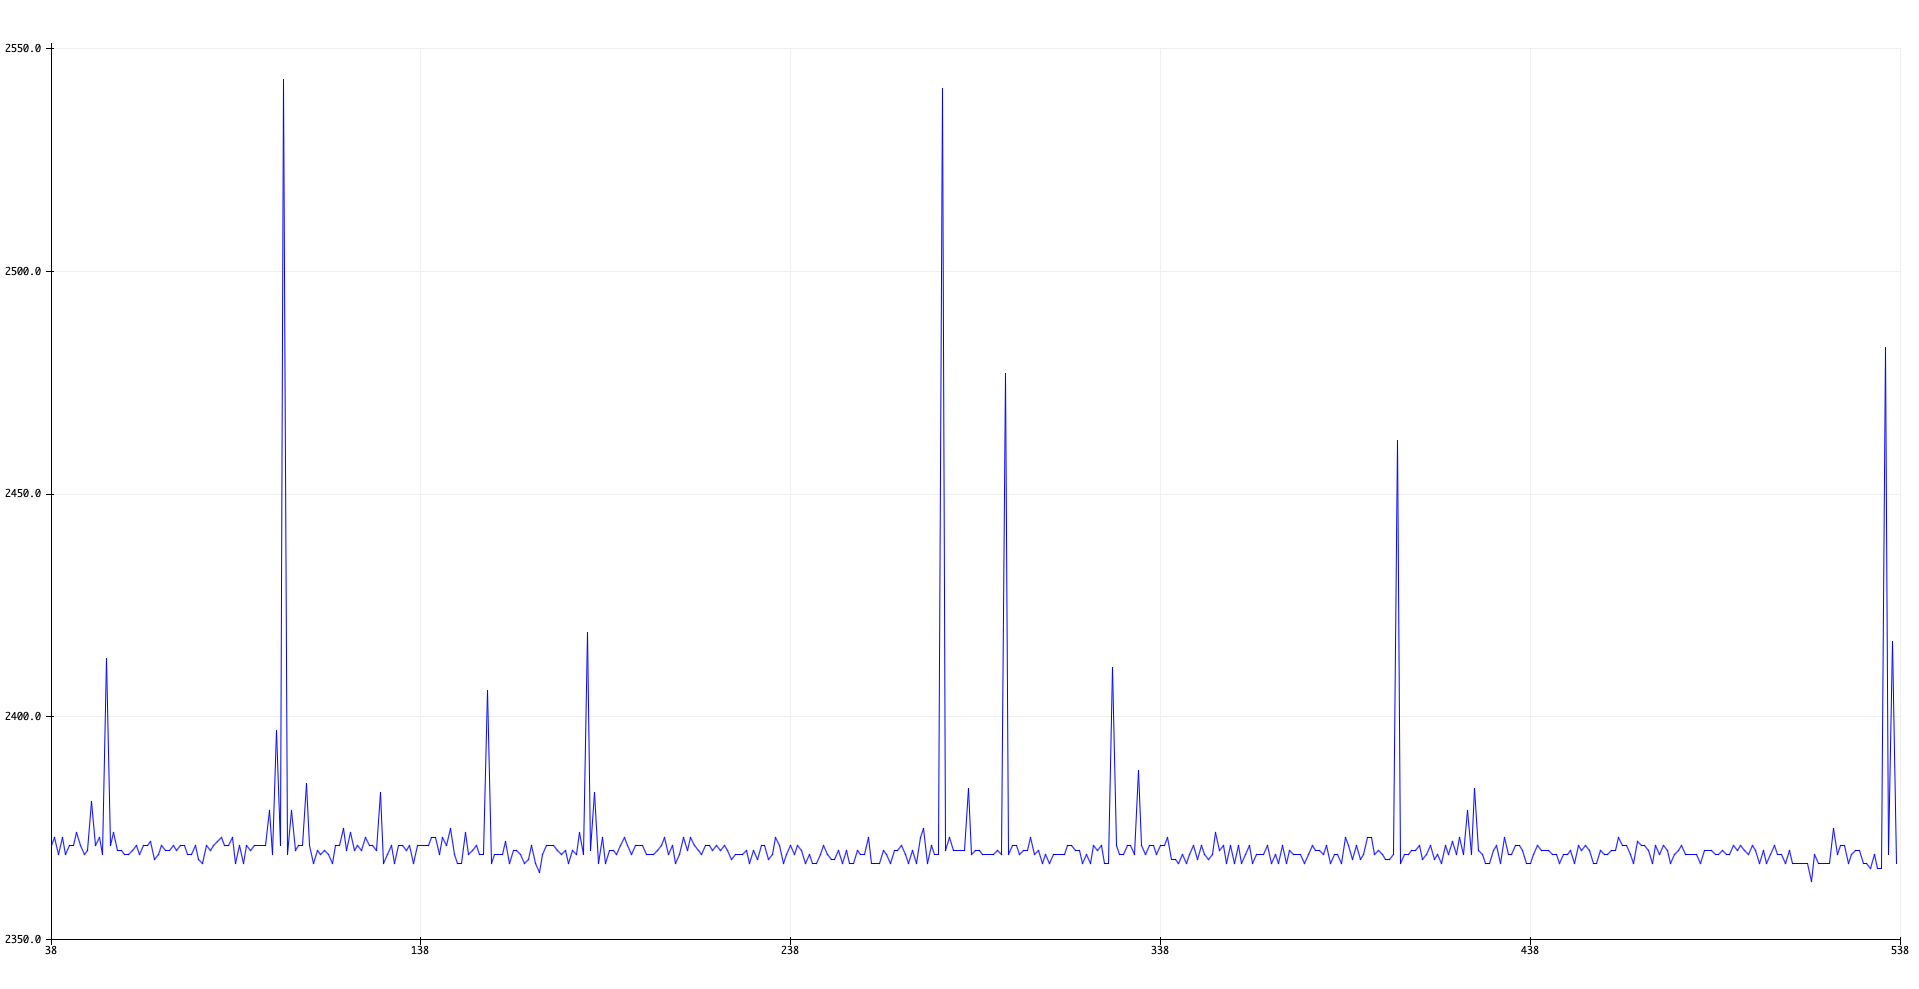
\includegraphics[width=10cm]{fig/m5core2_adc_raw}
    \caption{M5Stack Core2のADコンバーターの出力値の波形}
    \label{fig:m5core2_adc_raw}
  \end{center}
\end{figure}

移動中央値フィルター(Running Median Filter)は,平滑化を行うために時系列データの中からいくつかを抽出し(窓),その中から中央値を選ぶという処理を行うフィルターである.中央値には平均値よりも外れ値の影響を受けにくいという特徴があり,信号の平滑化に広く使われる移動平均フィルター(Running Median Filter)とは違い,外れ値が断続的に現れるデータにおいて影響を受けにくいという特徴がある.

今回のプログラムにおいてはRob Tillaart氏によるArduino用のライブラリ,RunningMedian\cite{tillaart_2021}を使用して実装を行った.移動中央値フィルターは窓の大きさを大きくするほど時間の遅れが生じるため,適切な窓の大きさを設定する必要があるが,今回はM5Stack Core2のADコンバーターの実際の出力値を見た上で,ライブラリが読み込むためのサンプル数を100個,窓のデータの数を5個として移動中央値フィルターを適用した.A-5Sの可変抵抗を調整することで意図的にADコンバーターの値を変動させたときの波形と,移動中央値フィルターを適用した値の波形を重ねたものを図\ref{fig:running_median_graph}に示す.

\begin{figure}[H]
  \begin{center}
    \caption{青線が元データ,赤線が移動中央値フィルター適用後}
    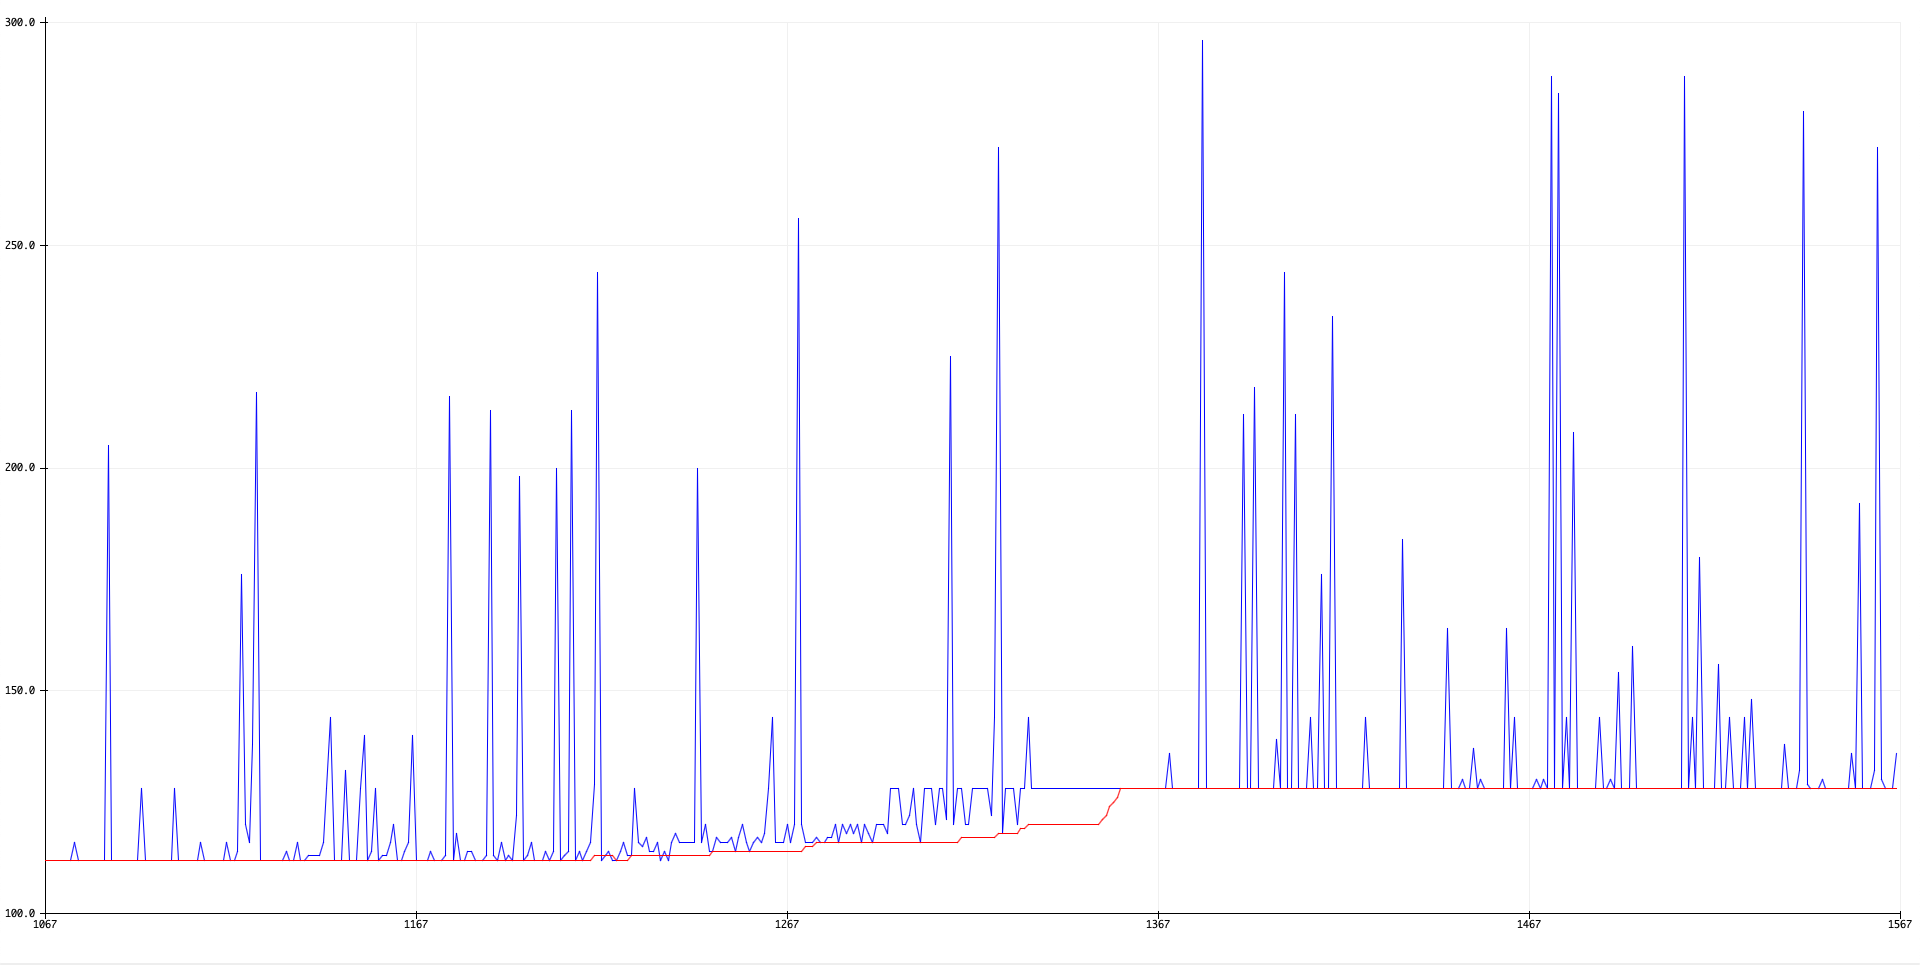
\includegraphics[width=10cm]{fig/running_median_graph}
    \label{fig:running_median_graph}
  \end{center}
\end{figure}

\subsection{呼気二酸化炭素の計測}

呼気二酸化炭素濃度は運動負荷によって変化し,安静時の約1\%から高強度運動時には9\%まで変化するという\cite{co2_percent}.そのため,運動中の呼吸代謝の測定にはこの範囲の二酸化炭素濃度の測定に対応する必要がある.

ところが,1万円程度以下で入手可能な市販の二酸化炭素濃度センサーは,測定範囲が0-5000ppm(0-0.5\%)のものが多い.今回は可能な限り高い運動強度での呼気二酸化炭素の濃度に対応するために,測定範囲が0-40000ppm(0-4\%)のSensirionの二酸化炭素センサーを用いたセンサーモジュールSCD30を使用した.M5Stack Core2とはI2C通信で接続を行った.図\ref{fig:scd30}及び表\ref{tb:scd30_specsheet}にSCD30とその仕様を示す.

\begin{figure}[H]
  \begin{center}
    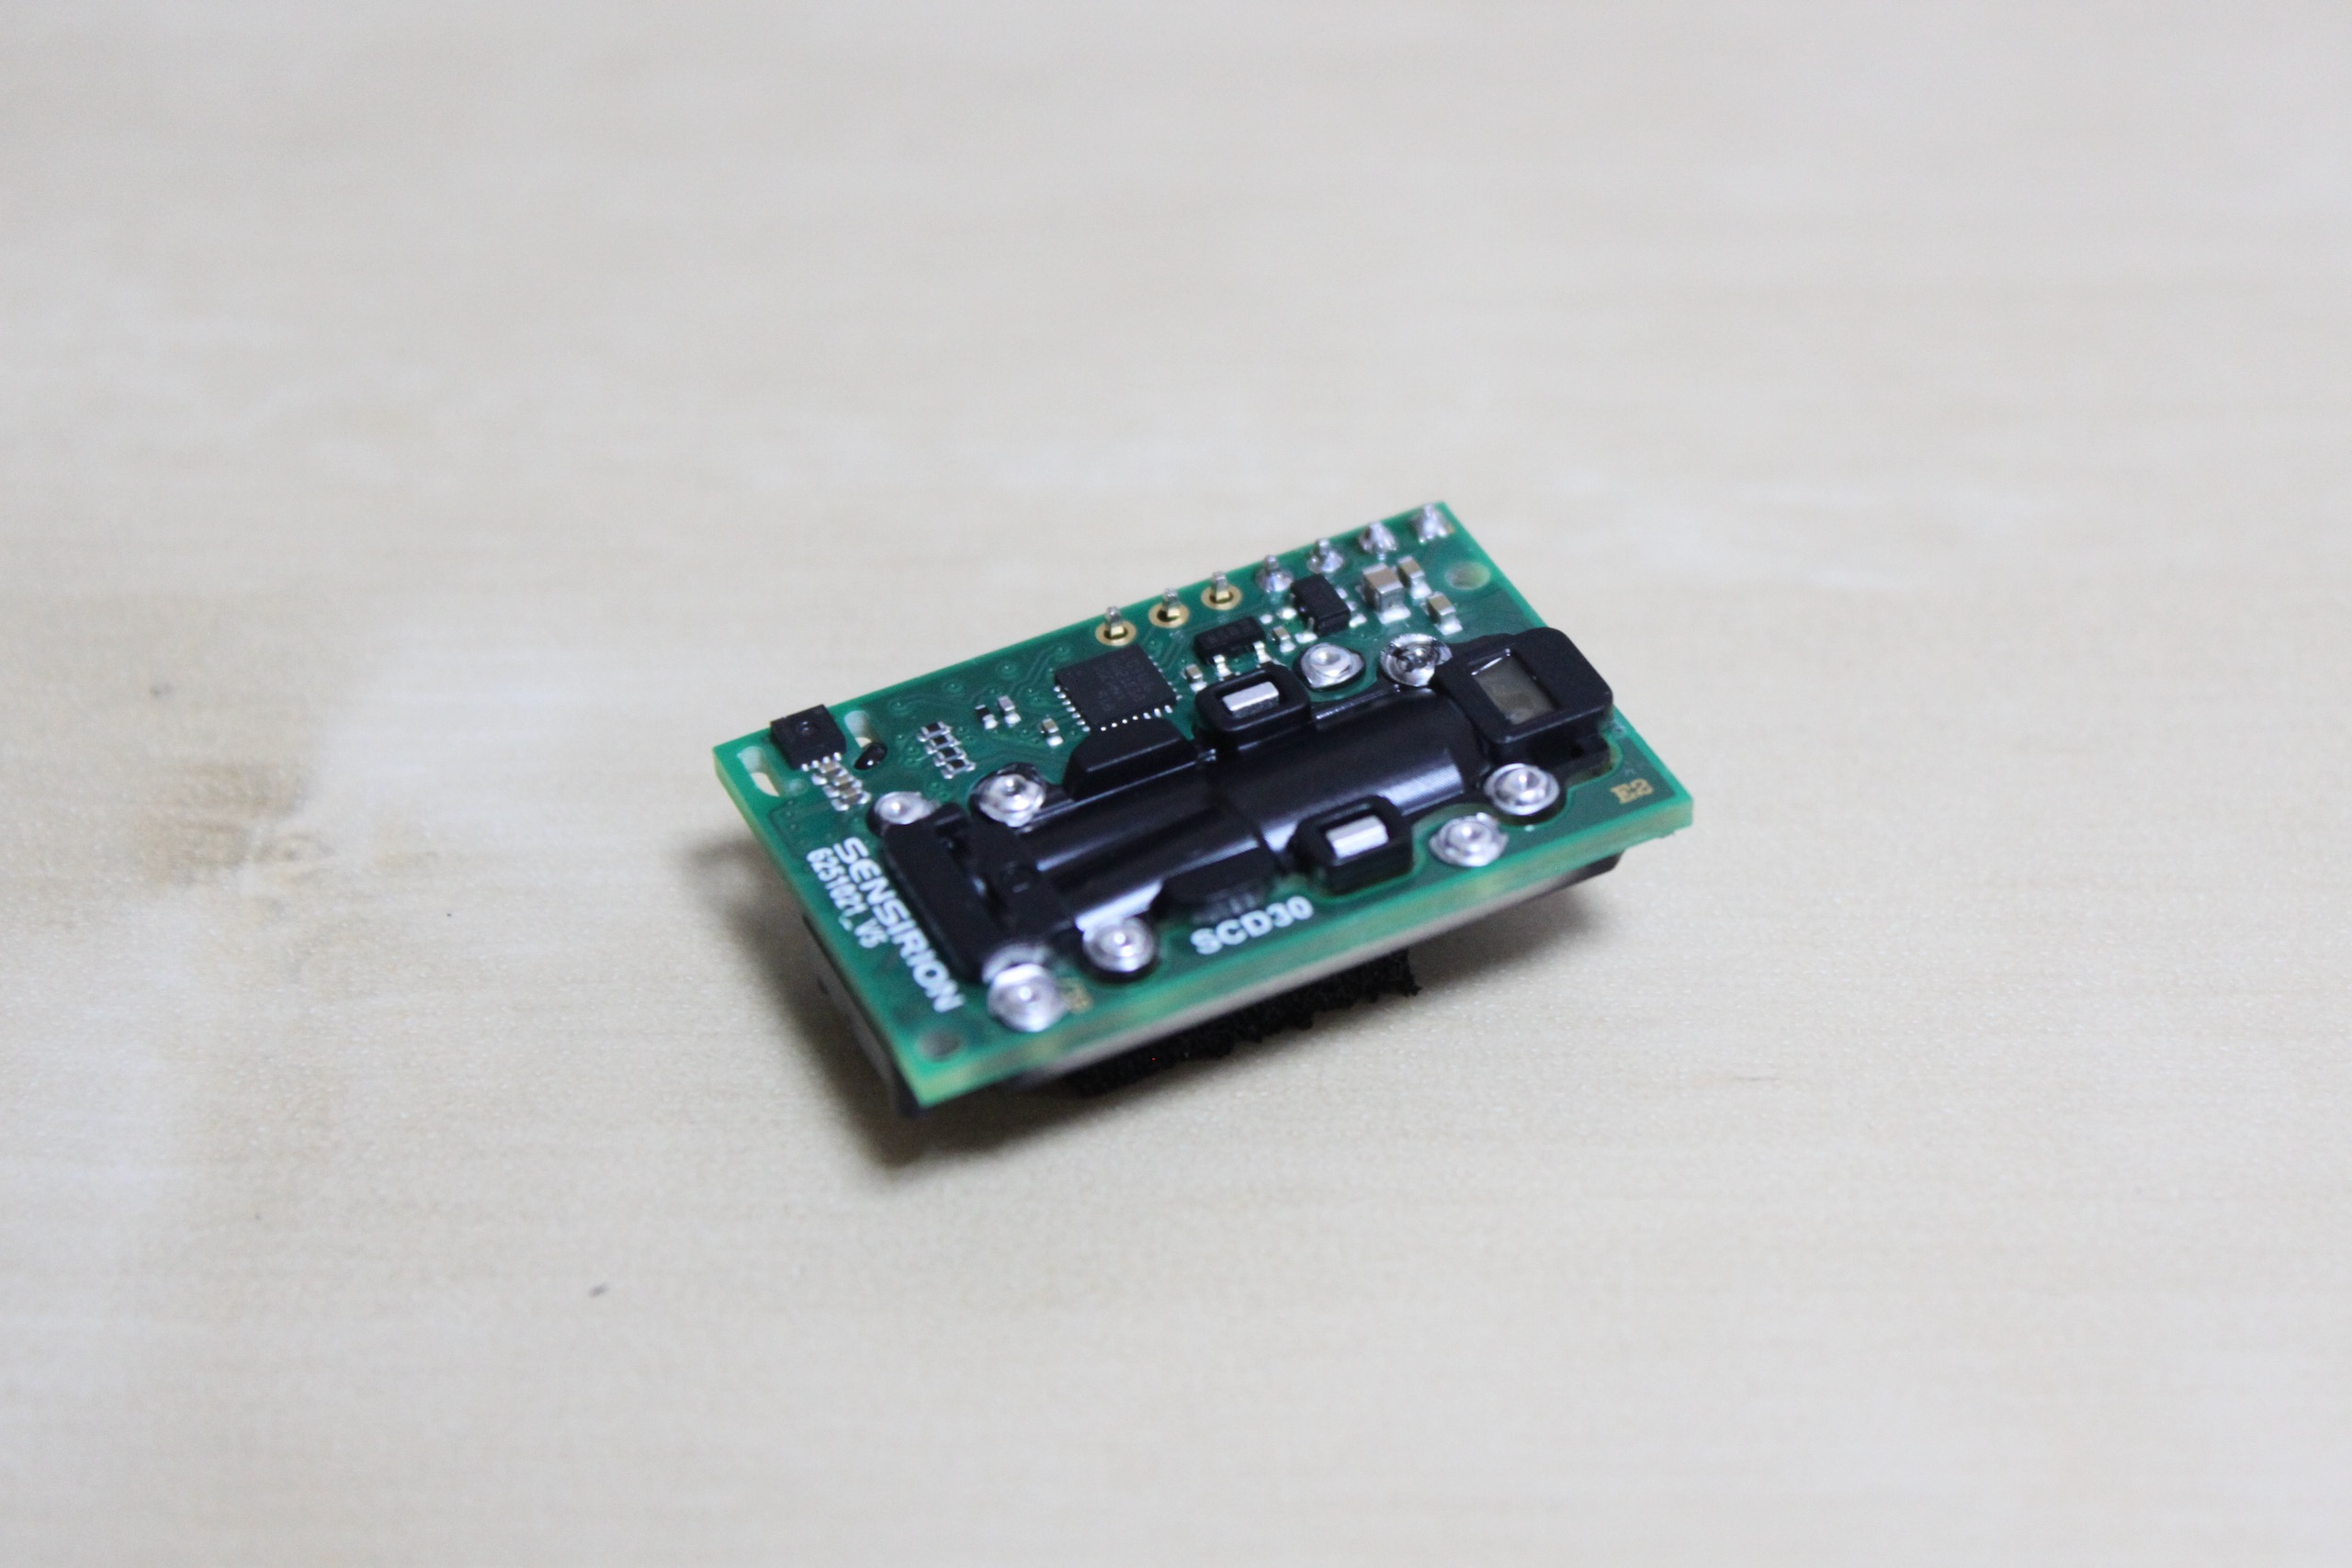
\includegraphics[width=8cm]{fig/scd30}
    \caption{SCD30}
    \label{fig:scd30}
  \end{center}
\end{figure}

\begin{table}[H]
\begin{center}
\caption{SCD30 主な仕様}
\label{tb:scd30_specsheet}
\begin{tabular}{|l|l|}
\hline
機能        & 二酸化炭素センサー,温度センサー,湿度センサー              \\ \hline
動作温度      & 0℃~+50℃                              \\ \hline
定格電圧      & 3.3V~5.5V                            \\ \hline
定格電流      & 17mA                                 \\ \hline
通信方式      & I2C,Modbus                           \\ \hline
サイズ       & 35mm \times 23mm \times 7mm          \\ \hline
CO2測定範囲,精度 & \begin{tabular}[c]{@{}l@{}}400ppm〜10000ppm,\pm(30ppm +3\%)\\ 10000ppm〜40000ppm (不明)\end{tabular} \\ \hline
湿度測定範囲,精度 & 0\%RH~100\%RH(25℃),\pm3\%RH          \\ \hline
温度測定範囲,精度 & 0℃~+50℃,\pm(0.4℃ +0.023×(T[℃] -25℃)) \\ \hline
消費電流      & 19mA @ 1測定/2秒                        \\ \hline
\end{tabular}
\end{center}
\end{table}

SCD30はNDIR方式(非分散型赤外線吸収方式)を用いて二酸化炭素の濃度を測定する.NDIR方式は,それぞれのガスが持つ特有の吸収波長領域を利用し,特定のガスのみの濃度を測定する測定方式である.ガス濃度測定方式のうち,対象ガスに変化を及ぼすことなく濃度を測定することができるのがNDIR方式の特徴である\cite{whats_ndir}.

SCD30にはセンサーの製造元であるSenserion他多数からArduino用ライブラリが用意されており,M5Stack Core2とI2C通信で接続を行い,数値取得用コマンドを送信することで容易にppm単位の二酸化炭素濃度を得ることが可能である.今回の装置では\%単位に変換して計算を行っている.

呼気を収集するミキシングチャンバー内は円筒形をしているため,3Dプリンターでミキシングチャンバーの形状に合わせた台座を製作し,酸素センサーとともに設置した(図\ref{fig:sensor_board}).



%二酸化炭素濃度を測定するセンサーにはMH-Z19Bを用いた.このセンサーはNDIR方式(非分散型赤外線吸収方式)を用いて二酸化炭素の濃度を測定する.NDIR方式は,それぞれのガスが持つ特有の吸収波長領域を利用し,特定のガスのみを対象ガスに変化を及ぼすことなく濃度を測定することができるガス濃度の測定方式である\cite{whats_ndir}.MH-Z19Bは,NDIR方式の二酸化炭素濃度センサーの中でも2000-5000円程度で比較的容易に入手できるものである.

%MH-Z19Bはコマンドを送信することで二酸化炭素濃度をppm単位で容易に取得することが可能である.今回はArduino用のライブラリを用いてppm単位の二酸化炭素濃度を取得し,\%単位に変換してVCO_2の計算に使用している.

\subsection{気温・大気圧の計測}
\label{sec:measuring_ambient}

STPD係数の算出に必要な気温・気圧は,BOSCHの温湿度・気圧センサーBME280を搭載したセンサーモジュールで計測する.BME280とM5Stack Core2間はI2C通信で接続を行った.BOSCH公式のほかいくつか用意されているArduino用のライブラリを用いることで,関数を用いて簡単に温度,湿度,気圧を取得することができる.今回はAdafruit製のArduinoライブラリを用いた.図\ref{fig:bme280}におよび表\ref{tb:bme280_specsheet}にBME280センサーモジュールとその仕様を示す.

\begin{figure}[H]
  \begin{center}
    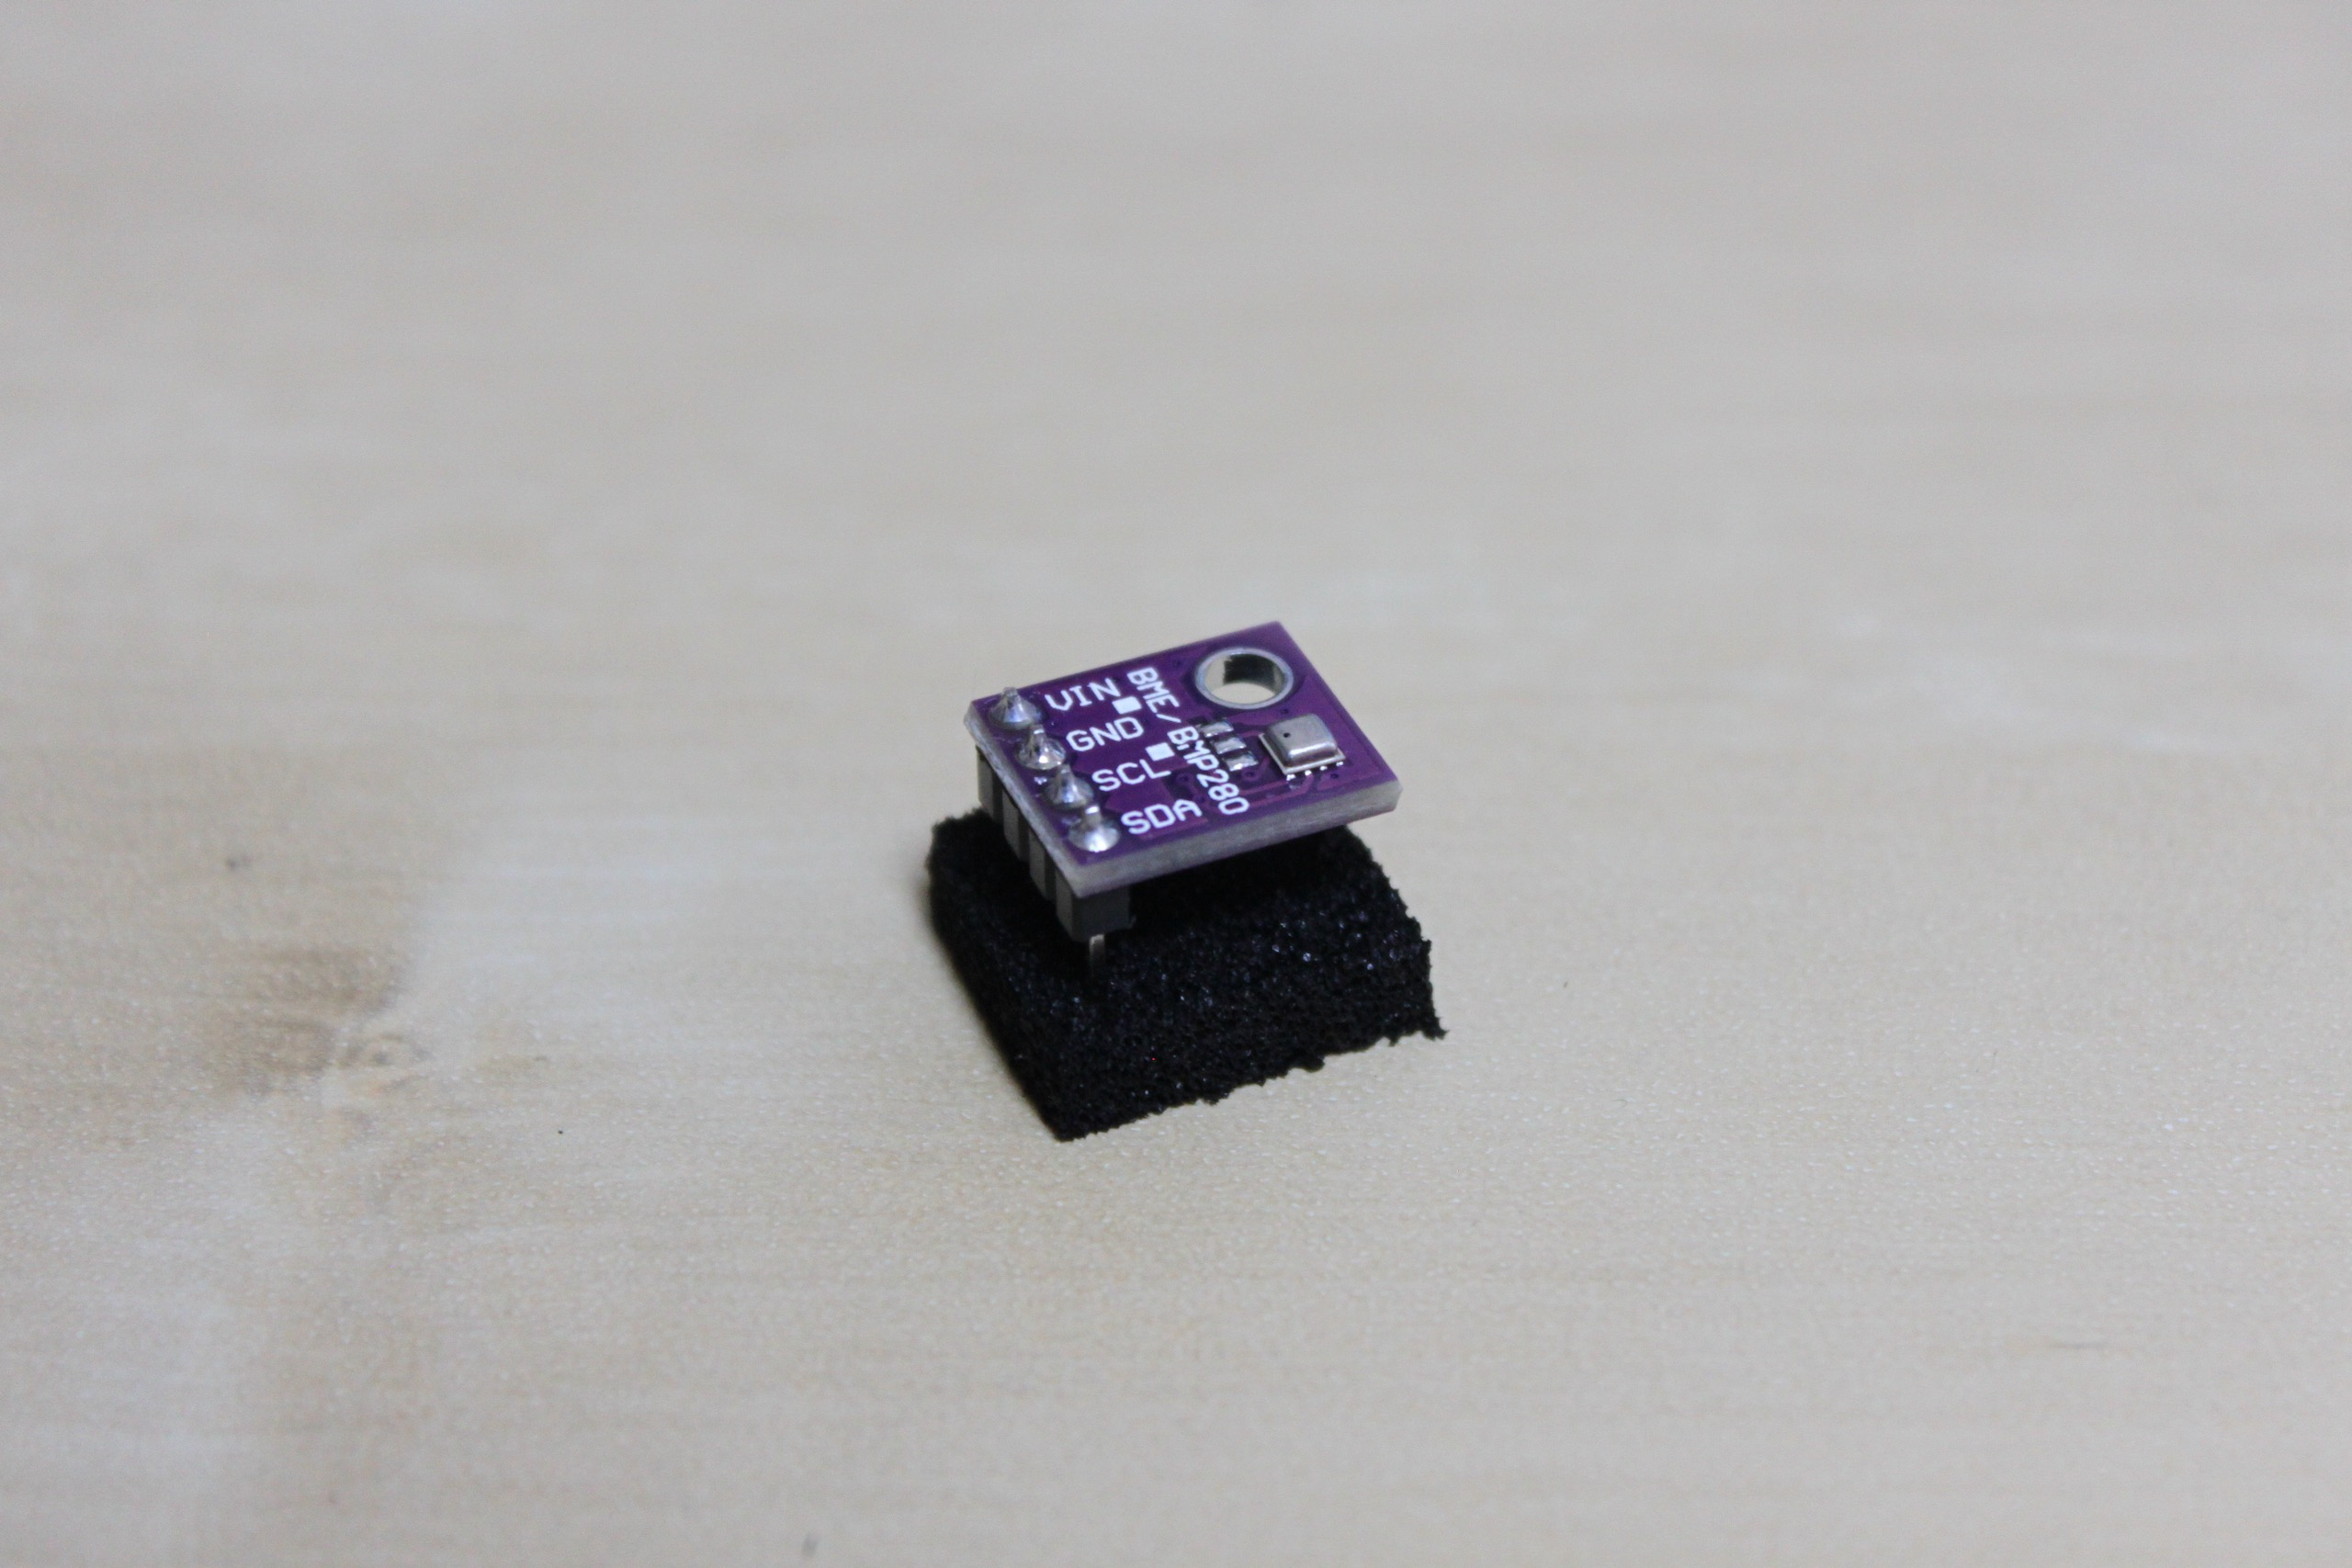
\includegraphics[width=8cm]{fig/bme280}
    \caption{BME280センサーモジュール.右下のチップがBME280本体である.}
    \label{fig:bme280}
  \end{center}
\end{figure}

% Please add the following required packages to your document preamble:
% \usepackage{multirow}
\begin{table}[H]
\begin{center}
\caption{BME280 主な仕様}
\label{tb:bme280_specsheet}
\begin{tabular}{|l|l|l|}
\hline
機能    & \multicolumn{2}{l|}{温度センサー,湿度センサー,気圧センサー} \\ \hline
電源電圧  & \multicolumn{2}{l|}{1.71V~3.6V}           \\ \hline
通信方式                                                                     & \multicolumn{2}{l|}{I2C(最大3.4MHz),SPI(3線式/4線式,最大10MHz)} \\ \hline
\multirow{3}{*}{\begin{tabular}[c]{@{}l@{}}測定範囲,\\ 精度,\\ 分解能\end{tabular}} & 温度                & -40~+85℃,\pm1℃,0.01℃                \\ \cline{2-3}
      & 湿度      & 0~100\%,\pm3\%,0.008\%          \\ \cline{2-3}
      & 気圧      & 300~1100hPa,\pm1hPa,0.18Pa      \\ \hline
基板サイズ & \multicolumn{2}{l|}{10 \times 18mm}       \\ \hline
\end{tabular}
\end{center}
\end{table}

センサーモジュールはM5Stack Core2が発する熱の影響を受けないように,本体筐体の外側に埋め込む形でネジで固定した(図\ref{fig:bme280_mount}).

\begin{figure}[H]
  \begin{center}
    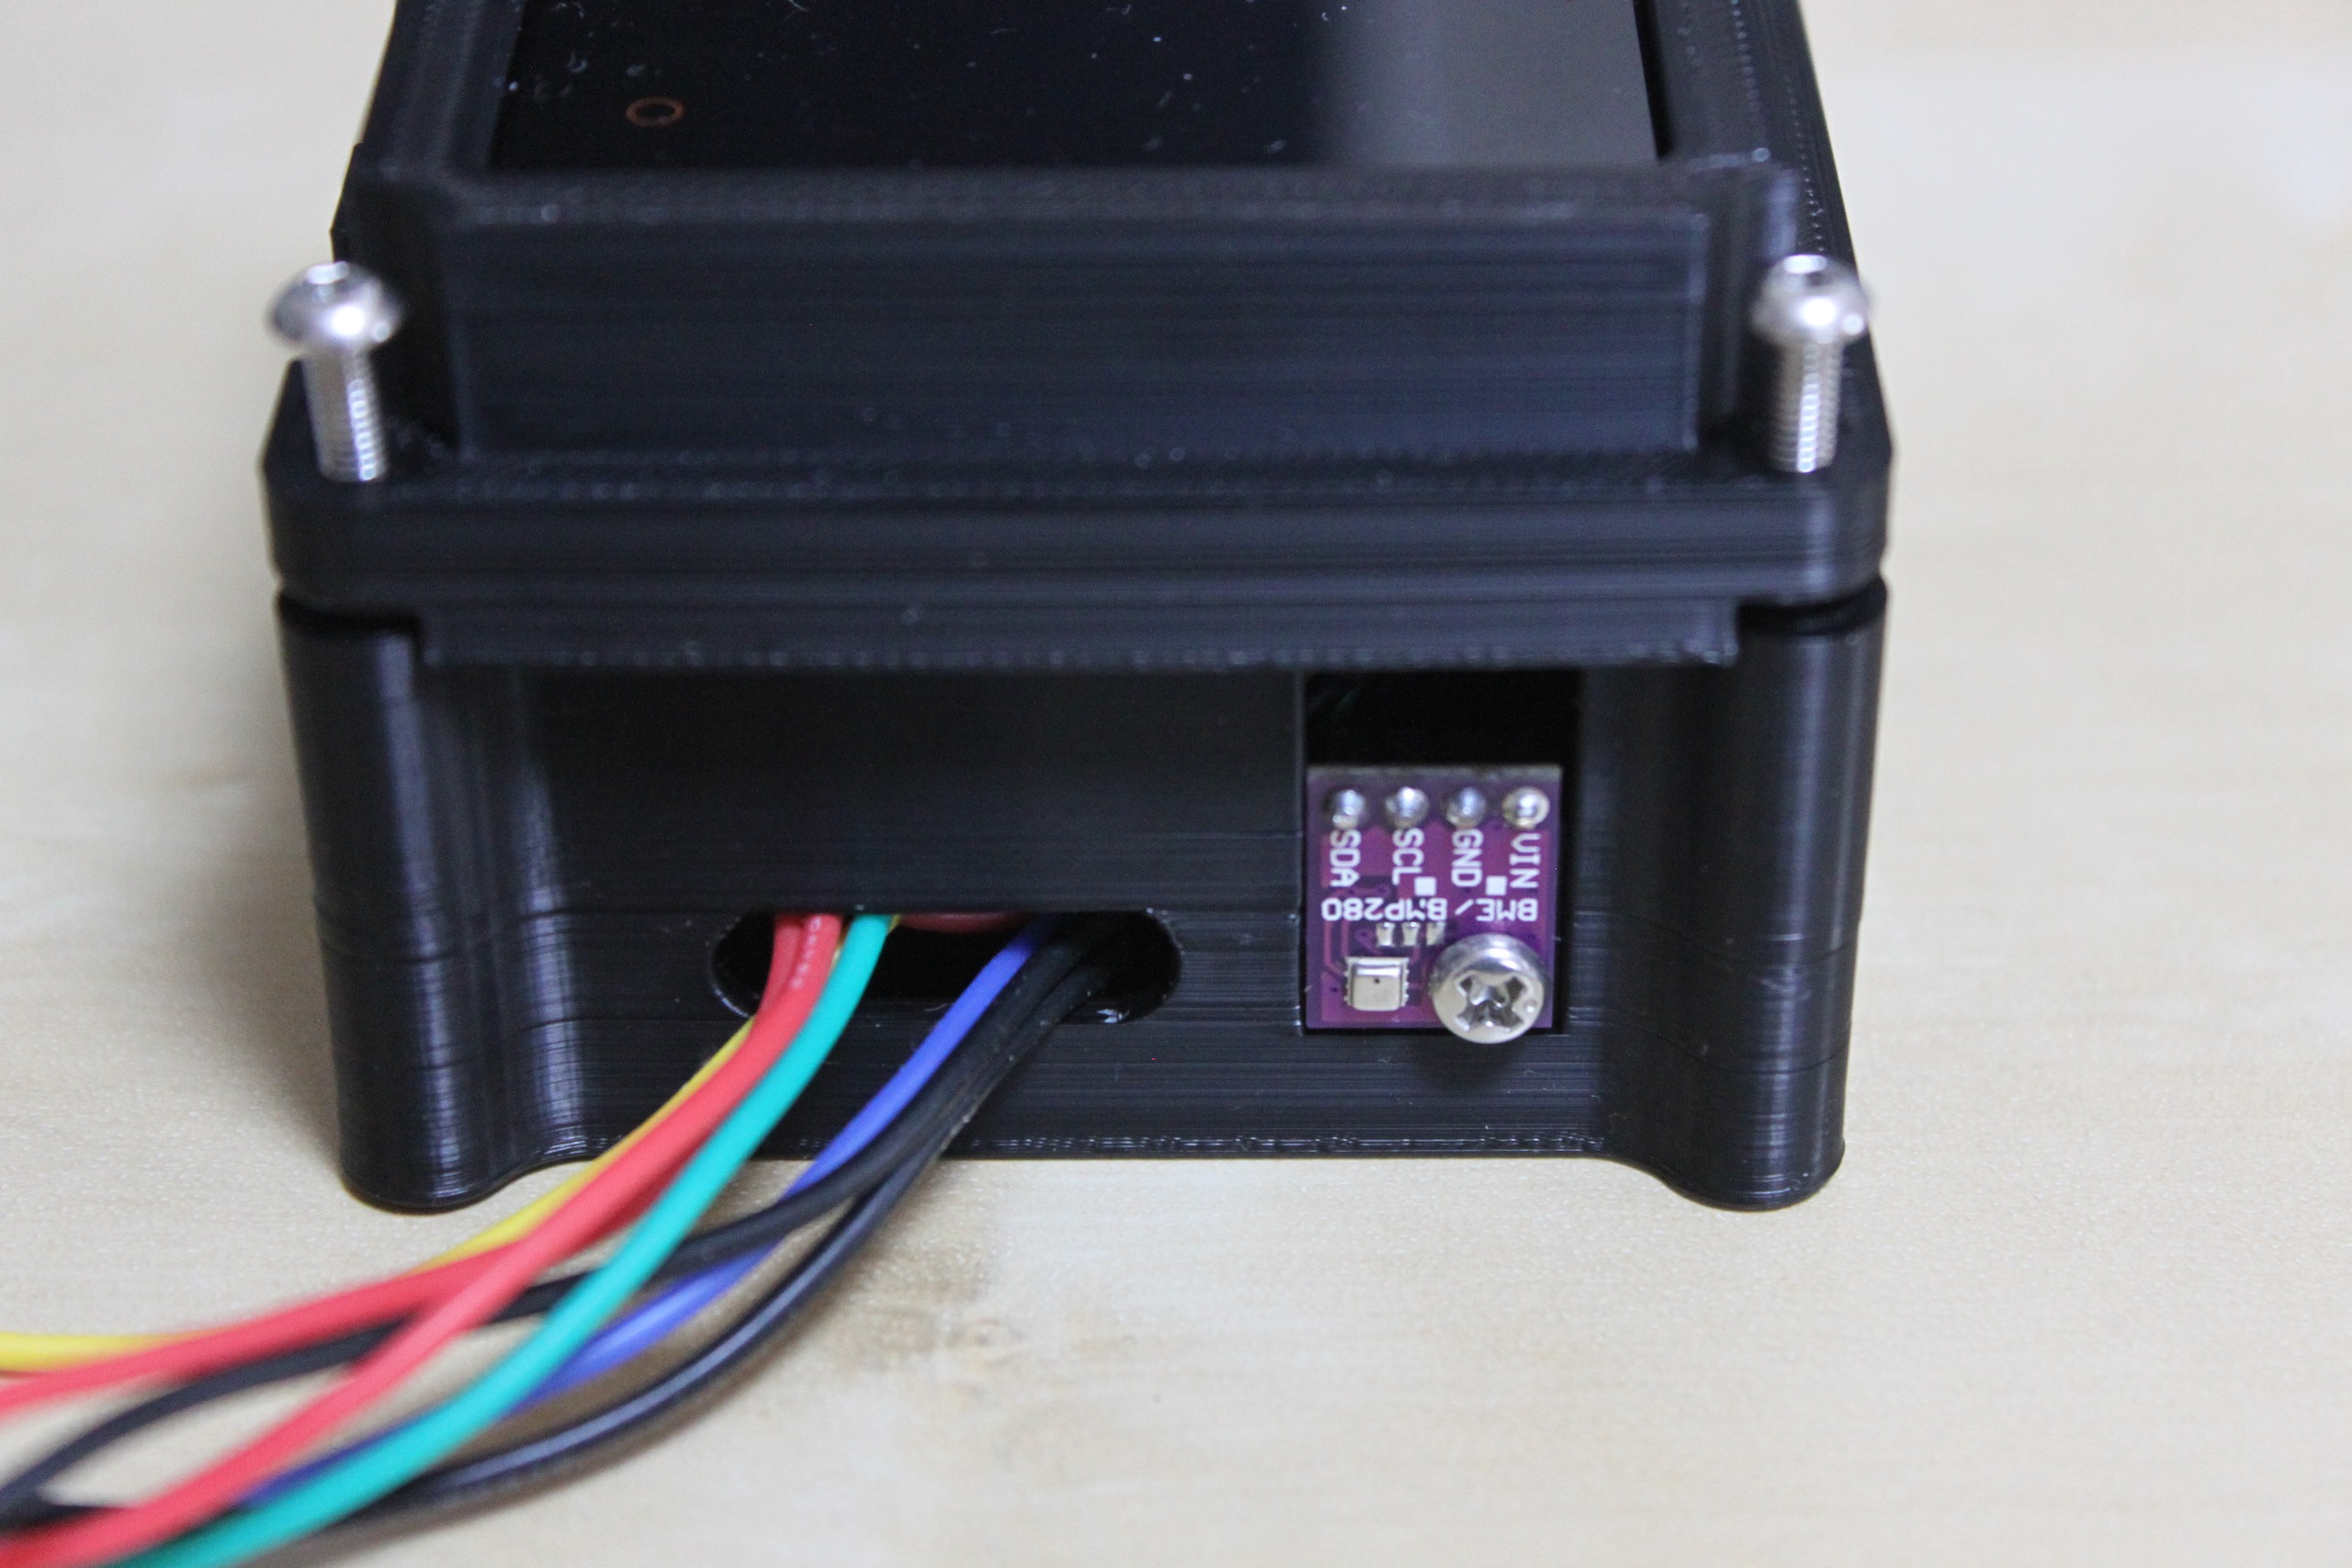
\includegraphics[width=8cm]{fig/bme280_mount}
    \caption{本体筐体に取り付けたBME280センサーモジュール}
    \label{fig:bme280_mount}
  \end{center}
\end{figure}

\subsection{データの記録}

\subsubsection{1分間平均値の計算}

呼吸代謝測定において計算に使用する数値は1分間平均値である.今回製作した装置は,リアルタイムでの数値の確認・記録を行えるようにするために,1秒ごとに1分間平均値を算出することとした.

気温,気圧に関しては,1分間平均値計算用の配列を用意し,毎秒新たなデータを配列に追加するとともに59秒前のデータを削除し続け,配列内のデータの平均を1秒ごとにとることで算出する.換気量,呼気酸素濃度,呼気二酸化炭素濃度に関しては,算出のための計算を出来るだけ整数値で行うために,それぞれパルス数,ADコンバーターの出力値,二酸化炭素濃度(単位:ppm)の1分間平均値を求め,1秒ごとにそれぞれを流量,酸素濃度,二酸化炭素濃度(\%)を求める方法で算出している.

\subsubsection{データの保存}

各センサーが測定した値,またそれを元に算出した値は,無線LAN経由でNTPサーバーから取得した現在時刻のスタンプと共にM5Stack Core2のTFカードスロットに挿入したMicro SDカードにCSVファイルとしてログデータを記録する.また,装置を使用する際には酸素センサーのキャリブレーションの他,ッカクセンサーの測定値が落ち着くまでしばらく待つ必要がある.この際にステータスの確認がしやすいように,1分間隔のデータをマイコンなどのログデータの記録に用いられるAmbientというサービスを用いてWebブラウザから確認できるようにした.

\subsubsection{レコードフラグの記録}

今回製作した装置ではデータの記録忘れを防ぐために,Micro SDカードを挿入している限りはデータを常時記録することにしている.長時間に及ぶ呼吸代謝測定を行う際は,後から測定データを利用する際に目的の箇所を見つけるのが難しくなることが想定される.そこで,M5Stack Core2の正面に3つ装備されているタッチボタンを利用して,CSVファイルに記録されるログデータにフラグを記録することができる機能を用意した.この機能をレコードフラグと呼ぶことにする.

\begin{figure}[H]
  \begin{center}
    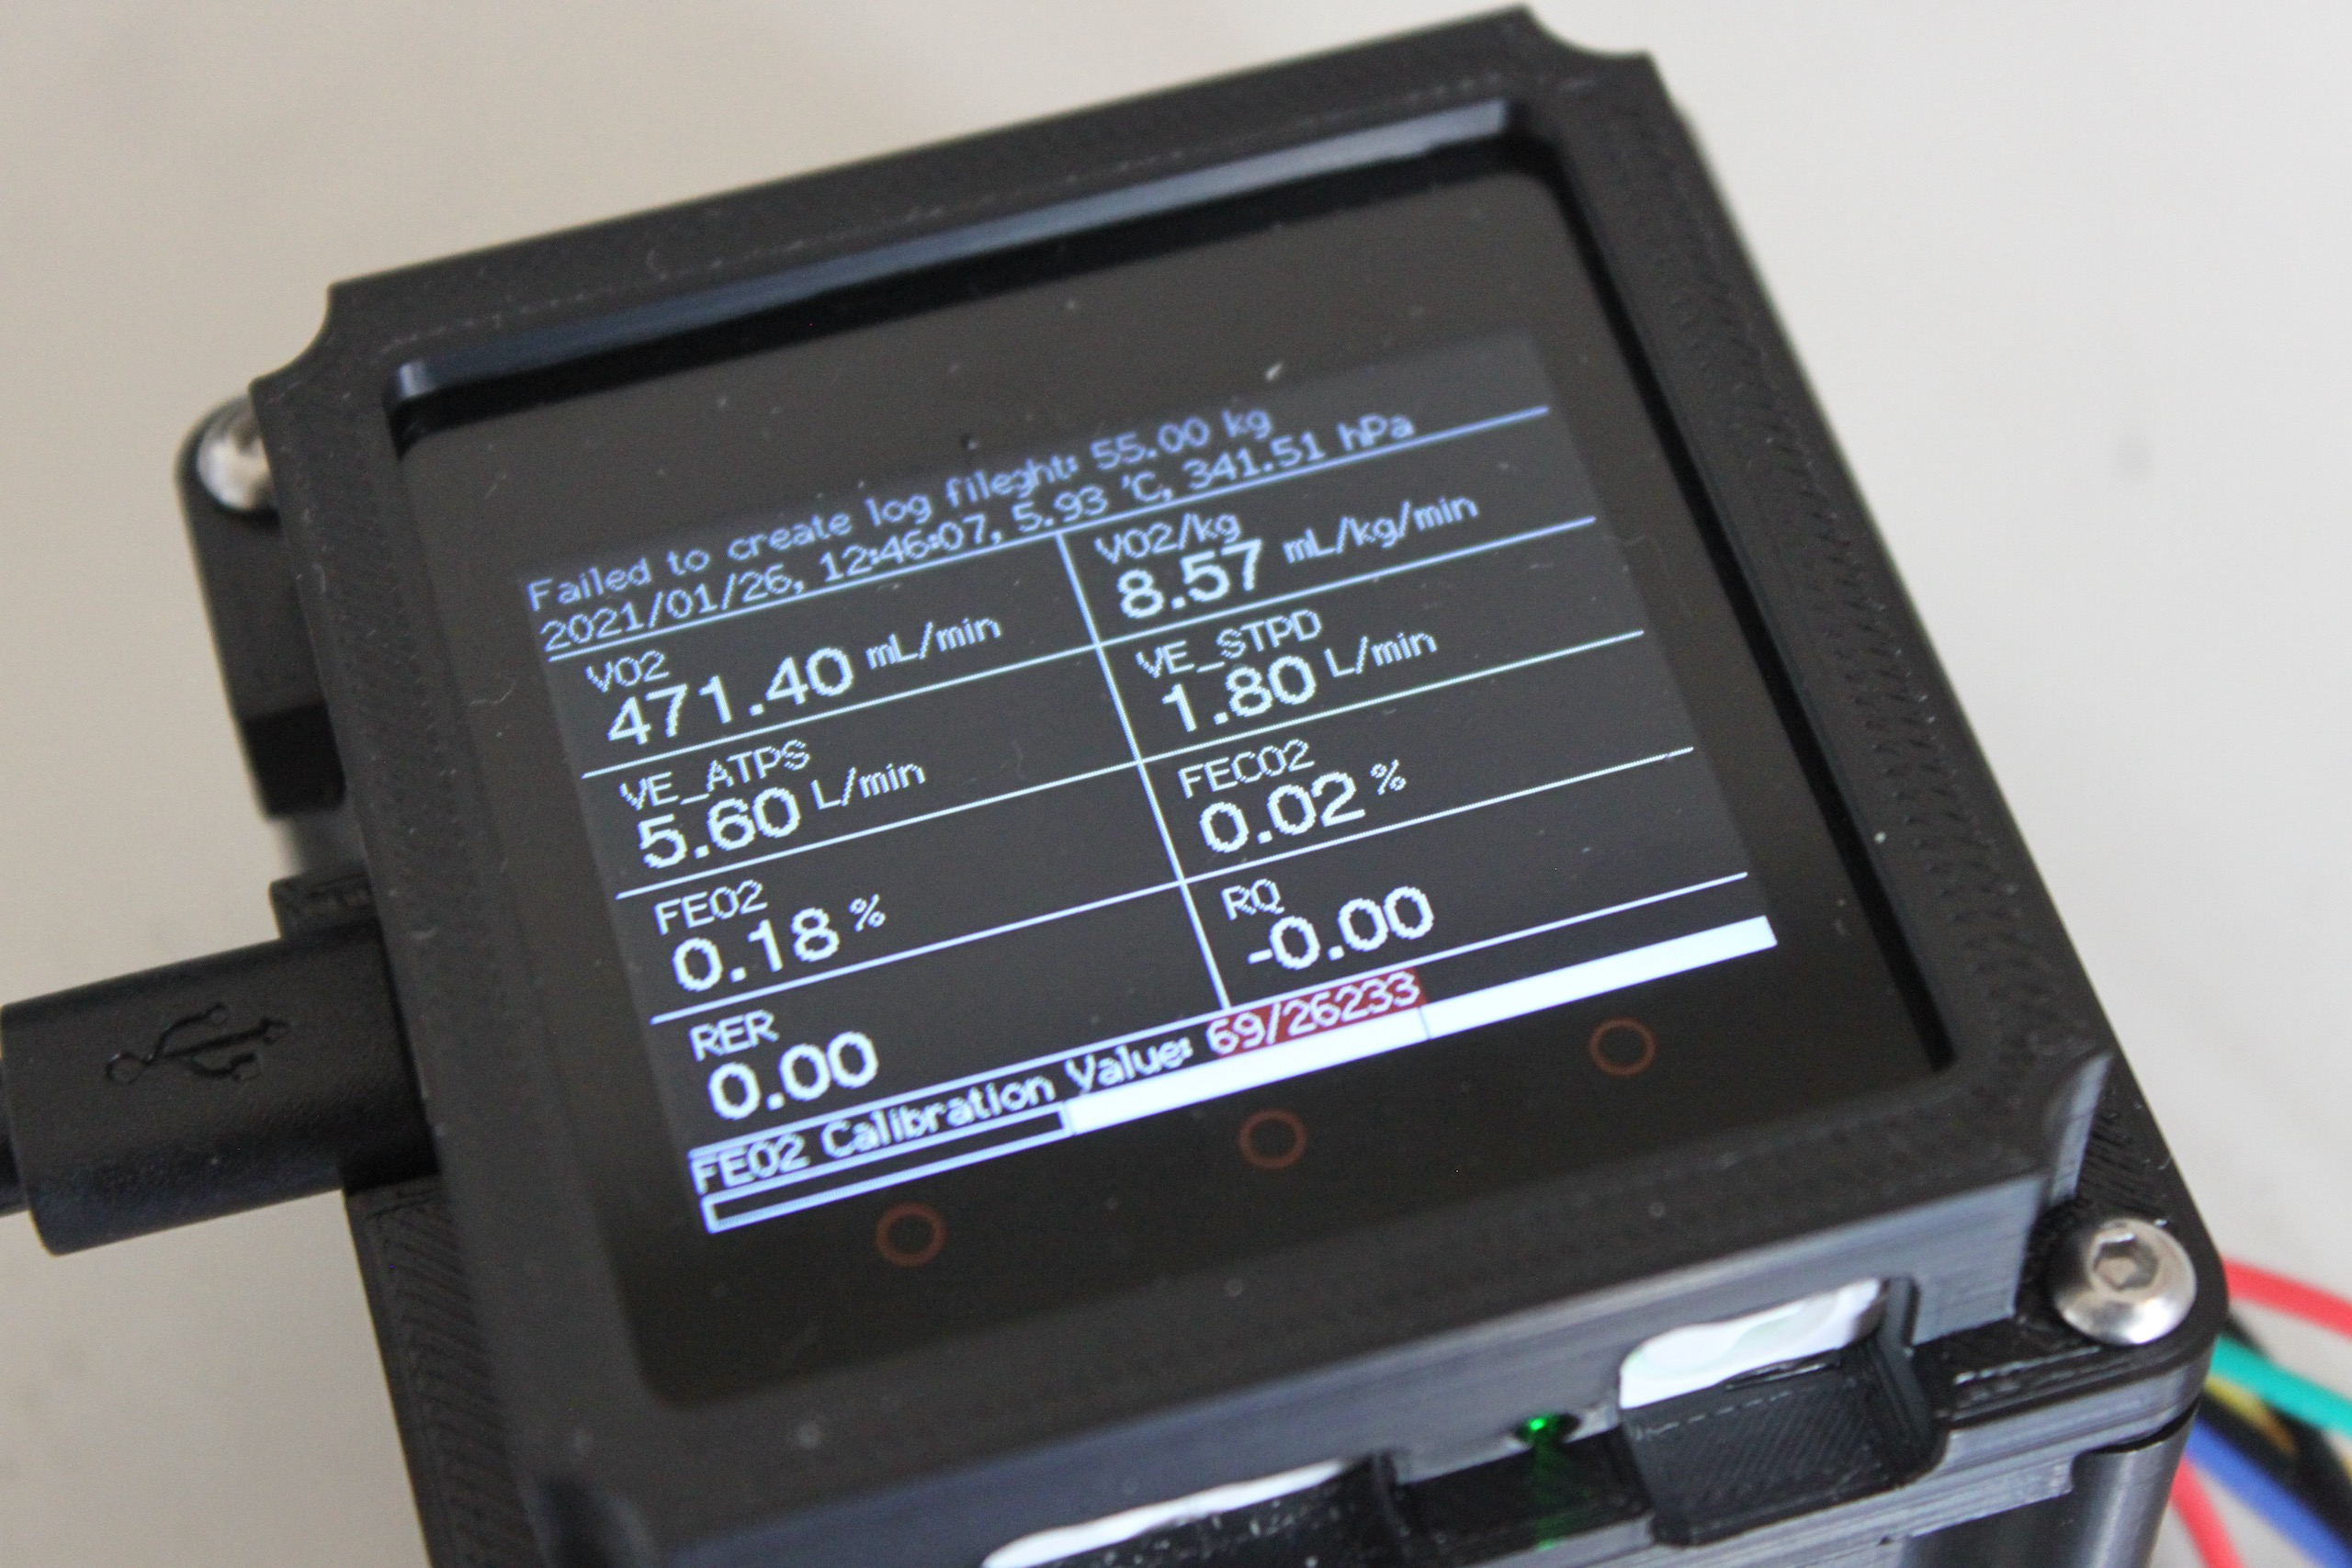
\includegraphics[width=8cm]{fig/record_flag}
    \caption{画面下部に表示されている白いバーがレコードフラグ}
    \label{fig:record_flag}
  \end{center}
\end{figure}

図\ref{fig:record_flag}の画面下部に表示されている白いバーがレコードフラグである.フラグはM5Stack Core2のボタンA,ボタンB,ボタンC,にそれぞれ対応してフラグA,フラグB,フラグCが存在する.起動時にはフラグは0になっており,ボタンをタップすることで1と0が交互に切り替わる.図\ref{fig:record_flag}の状態では,フラグBとフラグCが1になっている状態になっている.フラグは3つあり,それぞれが2通りの状態を持つので,8通りの状態をレコードフラグを用いて記録することができる.測定後にCSVファイルを処理する際に,このフラグを利用することで目的の箇所を見つけることが容易になる.

\subsection{使用部材と価格}

今回の装置の製作に使用した部材とその価格を表\ref{tb:price_of_material}に示す.なお,価格は購入時の価格を元に概算値で表記している.

\begin{table}[H]
\begin{center}
\caption{使用部材の品名と製品名,価格}
\label{tb:price_of_material}
\begin{tabular}{|l|l|l|}
\hline
品名         & 製品名              & 価格     \\ \hline
マイコン       & M5Stack Core2    & 5500円  \\ \hline
ミキシングチャンバー & CCレモン 1.5Lペットボトル & 150円   \\ \hline
ホース        & 洗濯機排水用延長ホース 1m      & 600円   \\ \hline
流量計        & YF-S201          & 1000円  \\ \hline
酸素センサー     & A-5S             & 1100円  \\ \hline
オペアンプ      & NJM2732D         & 100円   \\ \hline
二酸化炭素センサー  & SCD30            & 6000円  \\ \hline
温度・大気圧センサー & BME280           & 800円   \\ \hline
\multicolumn{2}{|l|}{合計}      & 15250円 \\ \hline
\end{tabular}
\end{center}
\end{table}

上記の表には価格の算出が困難なマスク,3Dプリンターで製作した部品に加え,元々所有していたものを使用したMicro SDカード,電子部品(ユニバーサル基板,配線,コンデンサー,抵抗など)などは含めていない.また,装置本体の価格としたため,流量計の校正に用いたシリンジは含めていない.それらを含めた場合,装置全体の価格は20000円程度になると思われる.

\expandafter\ifx\csname ifdraft\endcsname\relax
  \end{document}
\fi
